\documentclass[a4paper,11pt]{report}
\renewcommand{\baselinestretch}{1.3} 
\setcounter{secnumdepth}{3} % default value for 'report' class is "2"
\usepackage{fullpage}
\usepackage{breakcites}
\usepackage{todonotes}
\usepackage{graphicx}
\usepackage{natbib}
\usepackage{fixltx2e}
\usepackage{titling}
\usepackage{enumerate}
\usepackage{ftnxtra}
\usepackage{mathtools}
\usepackage{textcomp}
\graphicspath{ {images/} }
\usepackage{url}
\usepackage{amsmath}
\usepackage{xcolor,colortbl}
\usepackage{textcomp}
\usepackage{multirow}
\usepackage{amsmath}
\usepackage[toc,page]{appendix}
\usepackage{gensymb}
\usepackage{amssymb}

\widowpenalty 10000
\clubpenalty 10000

\begin{document}

\begin{titlepage}
\begin{center}
\Huge
\textbf{Using procedural methods to generate realistic virtual rural worlds}

\includegraphics[width = 400px]{uct_logo.jpg} \\
\large
\vfill
\emph{Minor Dissertation presented in partial fulfilment of the requirements for the degree of Master of Science in Computer Science} \\
\normalsize
\vfill
by \\
\Large
\vfill
\textbf{Harry Long} \\
\normalsize
\vfill
Supervised by: \\
\large
\vfill
James Gain and Marie-Paul Cani \\
\normalsize
\vfill
February 2016
\end{center}
\end{titlepage}

\chapter*{}
\begin{center}
\begin{minipage}{.6\textwidth}
\Large
\emph{I know the meaning of plagiarism and declare that all of the work in this document, save for that which is properly acknowledged, is my own.}
\normalsize
\end{minipage}
\end{center}

\tableofcontents
\listoffigures
\listoftables

%!TEX root = thesis.tex

\chapter{Introduction}
\par
Creating detailed virtual worlds can be a tedious task for artists. Indeed, modelling terrain, vegetation, water streams, rivers, water reserves, soil, rocks, buildings and road networks for large virtual worlds "by hand" can be extremely burdensome. This is especially true when realism is a key requirement. The increase in size and complexity of these virtual worlds mirror that of the processing capabilities of computing hardware. As a consequence, the task is only getting worse.\\

A popular technique to overcome the burden of repetitive tasks is to have them automated. This involves generating algorithms which, given a set of input parameters, generate the required content automatically. This is called \textit{procedural content generation} and has already been successfully applied in different areas of computer graphics including: the generation of non-repetitive textures \cite{Efros1999,Liang2001,Wei2009}, modelling plants \cite{Boudon2012,Fourcaud2008,Guo2011,Lewis1999}, generating terrains \cite{Smelik2009,Gain2009,Doran2010}, generating river networks \cite{Derzapf2011,Emilien} and generating city landscapes \cite{Gain,Kelly2007,Parish2001} (figure \ref{Example of procedurally generated content}) \\
A common difficulty with these methods, however, is finding the appropriate input parameters for the procedural algorithms. The correlation between the parameters and the resulting content is often unintuitive and, as a consequence, often comes down to iterative trial-and-errors until a "close enough" result is found. To overcome this, interactive techniques are often used in an attempt to make generating the input parameters more intuitive. These range from simple paint tools such as lassos and brushes \cite{Emilien} to sketch-based recognition algorithms \cite{Gain2009}. \\

\begin{figure}[h]
  \centering
	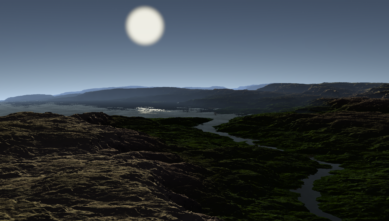
\includegraphics[natwidth=389,natheight=222]{procedural_generated_river.png}
	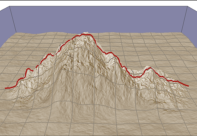
\includegraphics[natwidth=197,natheight=136]{procedural_generated_terrain.png}
	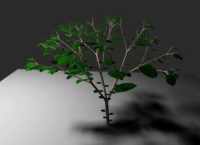
\includegraphics[natwidth=200,natheight=145]{procedural_generated_plant.png}
	\caption{Example of procedurally generated content. From top to bottom, left to right: Procedurally generated river stream \cite{Derzapf2011}, procedurally generated terrain through sketching \cite{Gain2009}, procedurally generated plant \cite{Soler2001}}
	\label{Example of procedurally generated content}
\end{figure}

The intent of this thesis is to develop procedural algorithms to automate the generation of virtual rural worlds. The input parameters for the procedural algorithms must be interactive and/or self-explanatory. 

\newpage
\section{Research Goals}

The research goals for this project are as follows:
\begin{itemize}
\item Develop procedural methods to automate the generation of realistic virtual rural worlds.
\item Provide intuitive and smart controls.
\item When possible, make interactions real-time.
\end{itemize}

One of the most important aspect of rural landscapes is vegetation. As such, our \textit{first goal} must strongly focus on the insertion of plants. The automation provided should not limit user control and the flexibility of the system. For example, it must be possible to generate worlds with varying elevations, river networks, water sources and vegetation.\\

For the \textit{second goal}, lots of thought must be put into making all user oriented controls intuitive. To do so, it will be important to research the pros and cons of other graphical applications in terms of control. If need be, multiple prototype controls should be developed in an attempt to find the best suited.\\

Maintaining a continuous feedback loop between user action and corresponding reaction is extremely important for both user-friendliness and to optimize usage. In an attempt to meet our \textit{third goal} therefore, efficient algorithms must be developed in order to keep there time complexity to a minimum. When suited, these algorithms should be developed to run on the GPU. \\

\section{Contributions}

The primary contributions of this thesis are:
\begin{itemize}
\item A carefully designed graphical interface permitting users to model any environment with minimal effort.
\item An efficient procedural water network generation algorithm which relies solely on soil, rainfall and terrain properties.
\item A novel vegetation generation component which uses clustering, statistical analysis and a simulator to ensure both realism and efficiency.
\end{itemize}

\section{Structure}

To start, a detailed overview of existing work is discussed in chapter \ref{chap:background}. To better understand the individual system components discussed within the body of this text, first an overview of the system is given. This is done in chapter \ref{chap:system_overview}. How the base terrain is specified, associated resources configured and water content procedurally generated is outlined in chapter \ref{chap:terrain_and_resources}. The clustering algorithm used to group vertices based on associated resources is discussed and its performance analysed in chapter \ref{chap:clustering}. Chapter \ref{chap:vegetation} discusses the techniques used to deduce suitable vegetation and efficiently generate highly detailed and large scale plant distributions. Test environments are generated and the systems strengths and weaknesses discussed in chapter \ref{chap:results}. Finally, chapter \ref{chap:conclusion} concludes this thesis and discusses future directions for this work.


%!TEX root = thesis.tex

\chapter{Background}

This chapter gives an overview of previous work related to our topic. Procedural methods applied to computer graphics is a wide area of research with an exhaustive number of publications. As a consequence, we cannot pretend to review all this work. Instead, we will focus on reviewing work which is closely linked to generating virtual \textit{rural} worlds. \\

We first present research which deals with the procedural generation of terrains. This will be followed by a review of methods to generate water flows on terrains. To conclude, an overview of techniques to generate vegetation will be presented.
\section{Rivers and Streams}

In this section will be reviewed the various techniques that are used to place rivers and streams on a terrain. We will split the review material into the following categories, each with dedicated sections: \textit{Classification-based}, \textit{Simulation-based}, \textit{Heuristic-based}, \textit{Fractal-based} and \textit{Explicit}. \textit{Classification-based} methods use pre-classified data based on real-world analysis to determine the most suited water network given a set of user-defined or terrain-defined constraints. \textit{Simulation-based} techniques attempt to simulate natural phenomena such as gravity to determine the water networks on a given terrain. \textit{Heuristic-based} techniques use algorithms based on real-world observation in an attempt to produce a plausible river network on the terrain. \textit{Fractal-based} techniques use recursive algorithms in their attempt to generate plausible river networks. \textit{Explicit} techniques require the user to specify in great detail the path the river should follow on the terrain.\\

The various techniques will be critiqued based on their realism, computational cost, the automation they provide and the amount of control the user has on the resulting scene. 

\subsection{Classification-based}

Classification-based methods use real-world analysis of river networks to determine, based on terrain parameters (slope, soil type, flow intensity, etc.), the types of rivers best suited (stream, cascade, rapid, etc.) to given landscapes.\\

Emilien et al \cite{Emilien2014} use classification-based techniques in their research focused on the lesser explored area of procedurally generated waterfall scenes. They model waterfalls as three separate segments: \textit{running water}, \textit{free-fall} and \textit{pool}. \textit{Running water} segments are parts of the water network in continuous contact with the terrain. \textit{Free-fall} segments are parts which break terrain contact (i.e. waterfall). Lastly, \textit{pool} segments represent the water-basin formed where free-fall segments meet the terrain. \\
Given a terrain, the user models running water and pool segments by defining control points and free-fall segments by defining a parabola. The control points for the running water and pool segments are not constrained to being in contact with the terrain as the terrain will adapt accordingly. The only constraint is that the path must continuously flow downhill. Based on this input, the system calculates plausible water flow intensities which, if required, can be overridden by the user for finer control.\\
The slope and water flow intensity requirements are then used as input to the waterfall classification (figure \ref{fig:waterfall_classification}) in order to determine realistic waterfall scenes to generate.\\

\begin{figure}[h]
  \centering
	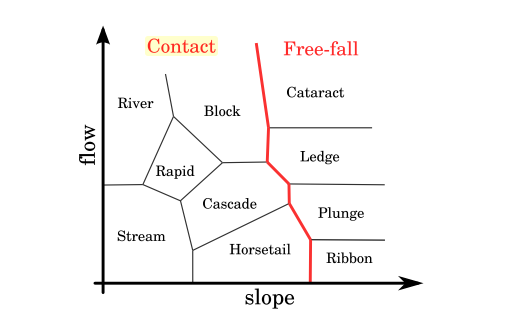
\includegraphics[]{waterfall_classification.png}
	\caption{\textit{Waterfall classifications \cite{Emilien2014}}}
	\label{fig:waterfall_classification}
\end{figure}

By automatically generating plausible waterfall scenes based on trajectory input from the user, the technique strikes a good balance between automation and user control. In terms of computational complexity, the work by Emilien et al \cite{Emilien2014} is able to produce complex waterfall scenes in near real-time.

\subsection{Simulation-based: Gravity} \label{subsec:gravitation}

Gravity simulating techniques attempt to determine the path water will take on a terrain by algorithmically replicating the effects of gravity. \\

In order to generate plausible rivers, Belhadg et Audibert \cite{Belhadj2005} simulate the effect gravity has on water particles placed on the peaks of pre-generated ridges. To create the ridges, particle pairs are first placed at random locations on the terrain. These particle pairs are then randomly assigned a horizontal axis from which they iteratively distance themselves in opposite directions. At each iteration a new vertex is placed and its height decreased from the previous vertex based on a Gaussian distribution. To create the river networks, river particles are placed on the top of these generated ridges and a physical simulation which takes into consideration particle velocity, particle mass and surface friction is used to model the motion of these particles on the terrain. The path followed by these particles is tracked and, when two paths intersect, their particle velocity and mass are combined. When all particles have stopped moving the simulation is deemed balanced and all particle paths which do not lead to terrain extremities discarded. The remaining particle paths are kept and form the core river network. \\

Similarly, in the work by Soon Tee \cite{Teoh2008}, water is placed at specific locations on the terrain either by the user or whilst simulating rainfall. To determine the course the placed water takes on the terrain, water is iteratively evacuated into the surrounding cell with lowest elevation. This continues until a local minima or terrain extremities is reached.\\

In their work on modelling the effects of hydraulic erosion, Št'Ava et al. \cite{StAva2008} determine the course user-placed water takes on the terrain using a hydrostatic pipe-model simulation. In order to do so, the terrain is split into equal-sized (configurable) columns and the simulation iteratively evacuates water from source to surrounding destination columns based on column elevations, fluid density and gravitational acceleration. \\

These techniques can produce very plausible results but have the downside of being dependent on the base terrain as their height-field must cater for river networks in the first place. This is not the case, however, for the work by Št'Ava et al. \cite{StAva2008} for which the gravitation simulation is used as a feedback loop to model terrain erosion. The performance of these methods depend heavily on the level of detail of the underlying water flow simulation. Št'Ava et al. \cite{StAva2008}, for example, succeed in generating the water flow in real-time by optimizing their algorithms to use the heavily parallel architecture of GPUs.

\subsection{Simulation-based: Erosion}

Erosion-based simulations attempt to produce realistic terrains by modelling the effects of erosion. Erosion results from exogenic processes (water flow, wind, temperature) and is characterised by the removal of soil and rock from one location on earth's surface to be redeposited on another. Earth's landscape is a direct consequence of erosion and reproducing this phenomena accurately is core to procedurally generating accurate landscapes. Both Kelly et al. \cite{Kelley1988} and Št'Ava et al. \cite{StAva2008} attempt to produce plausible terrains by modelling these effects.\\

In the work by Kelley et al. \cite{Kelley1988}, the user specifies, on a horizontal plane, the terrain outline along with the main trunk stream. The terrain outline is used to configure the terrain extremities once ported to a three-dimensional space. The main trunk stream specifies the path which the highest order water stream should follow on the resulting terrain. Given this terrain outline and the position of the initial main trunk stream, the system iteratively increments the number of nodes which form the main trunk in order to add streams to the network. The number of new nodes added depends on the drainage area (surface area that a stream needs to channel) and the soil type as more resistant soil materials (e.g. stone) will be less influenced by water erosion than weaker ones (e.g. clay). \\

Št'Ava et al. \cite{StAva2008} are able to simulate the effects of hydraulic erosion on a terrain in real-time by using the massively parallel architectures of GPUs. Virtual pipettes are used by the user to drop water at required locations on the terrain and a gravitation simulation mentioned previously (\ref{subsec:gravitation}) is used to determine the initial water course on the terrain. Whilst the water is being routed through the terrain, the effects of \textit{force-based} and \textit{dissolution-based} erosion are simulated. \textit{Force-based} erosion is a direct consequence of the the force of the water on the terrain surface (figure \ref{fig:force_based_erosion}). Dissolution-based erosion is a consequence of the water mass on the terrain surface under the water and is most often characterised by a smoothing effect (figure \ref{fig:dissolution_based_erosion}).\\

\begin{figure}[h]
  \centering
	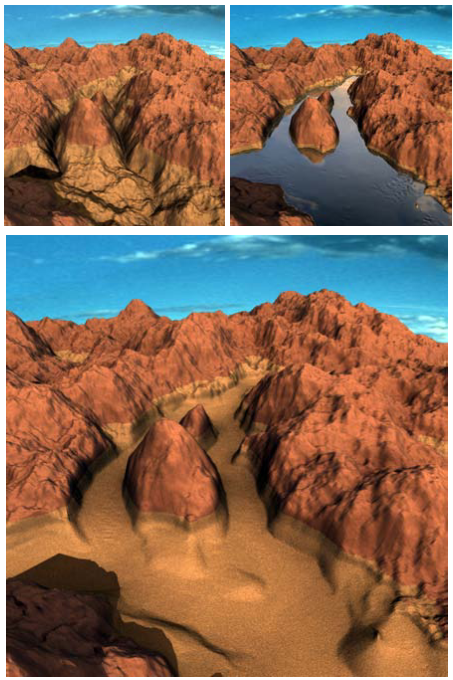
\includegraphics[scale=0.5]{dissolution_based_erosion.png}
	\caption{\textit{Simulation of dissolution-based erosion erosion caused by water movement\cite{StAva2008}}}
	\label{fig:dissolution_based_erosion}
\end{figure}

\begin{figure}[h]
  \centering
	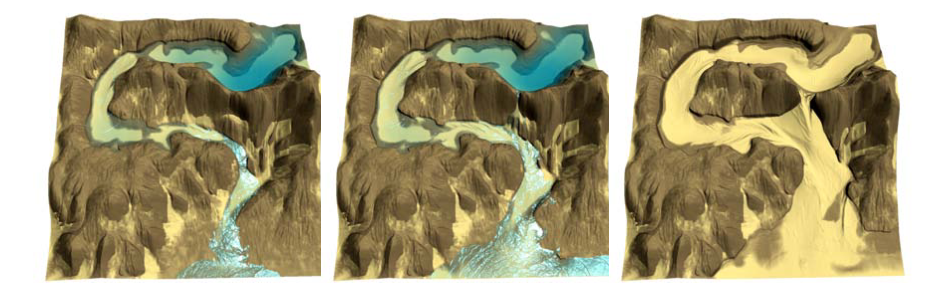
\includegraphics[width=\textwidth]{force_based_erosion.png}
	\caption{\textit{Simulation of the effect of force-based erosion caused by running water \cite{StAva2008}}}
	\label{fig:force_based_erosion}
\end{figure}

Whether modelling erosion indirectly like in the work by Kelley et al. \cite{Kelley1988} which builds the terrain around models of erosion or directly like the work by Št'Ava et al. \cite{StAva2008} which simulates the effect of erosion in real-time, both succeed in producing plausible terrains with integrated river networks. Fine-control over the resulting terrain, however, is limited in the work by Kelley et al. \cite{Kelley1988} due to extensive automation. This is overcome in the work by \cite{StAva2008} et al. by permitting the user to place water using a virtual pipette and remodel the terrain relief on-the-fly. In terms of computational cost, Št'Ava et al. \cite{StAva2008} are able to reproduce the effects of erosion in real-time.  

\subsection{Simulation-based: Rainfall}

In order to determine where on the terrain rivers will appear, work by Soon Tee \cite{Teoh2008} performs a rainfall simulation to determine both the location and quantity of water at different points on the terrain followed by a gravitation simulation (mentioned above) to determine the course of the water on the terrain. The rainfall simulation requires the user to specify wind direction and maximum rainfall. Then, starting from the source of the wind, the system simulates clouds moving in the direction of the wind with a configured velocity. When contact is made with points on the terrain, water is dropped on the corresponding cell. The amount of water dropped increases with altitude and zeroes out when all available rainfall is depleted. \\

Simulating rainfall in order to determine where water will fall on the terrain and therefore where river networks will form is an original approach and one that successfully generates visually plausible terrains. Requiring only wind direction, wind velocity and maximum rainfall from the user, the system provides a good level of automation. Determining the influence these inputs have on the resulting scene could be unintuitive however, and require a "trial-and-error" approach. Their algorithm creates the terrain along with the river networks in O(n) time, n representing the number of cells on the terrain.

\subsection{Heuristic-based}

Heuristic approaches attempt to build river and stream networks on terrains by algorithmically reproducing key characteristics based on real-world observations. \\

Derzapf et al. \cite{Derzapf2011} use such methods in their work based on procedurally generating virtual planets in real-time. To do so, only a very basic mesh-representation of the terrain is generated at first and detailed content is generated on demand as the user navigates through the virtual world. This method of adaptive rendering permits memory usage to me manageable whilst not compromising on realism. To ensure updates are performed in real-time, their algorithms are designed to make use of the massively parallel architecture of GPUs. \\
To initialise the base representation of the planets, the system first creates the base mesh with all vertices representing the sea. The system then randomly assigns a certain number of these vertices to act as seed continent vertices to spread until a user-configured land-to-water ratio is reached.
To place rivers, similarly to the work by \cite{Genevaux2013} et al., they first locate continental points which are on coastal edges to act as river mouths. When such a vertices are found, adjacent continental vertices are iteratively selected pseudo-randomly and connected in order to form the river network. \\
To assign ground altitudes to connected river vertices the system employs the following formula, starting from the river mouth:

\begin{center}
$a_{v} = a_{u} + e_{a}l_{e}\xi , e_{a} = \frac{a_{maxriver}}{l_{r}} $ \\
\end{center}

Where:
\begin{itemize}
\item $a_{v}$ is the ground altitude of the current vertex.
\item $a_{u}$ is the ground altitude of the previously processed vertex (or zero if \textit{v} is the first vertex).
\item $e_{a}$ is the average ground elevation.
\item $l_{e}$ is the length of the current vertex.
\item $\xi \in [0,1[$ is a uniformly distributed pseudo-random number.
\item $a_{maxriver}$ is the user-configured maximum river altitude.
\item $l_{r}$ is the current river length.
\end{itemize}

When the ground altitudes have been assigned, the following formula is used iteratively on each river vertex to assign water altitudes:

\begin{center}
$w_{v} = a_{v} + e_{w}l_{e}, e_{w} = \frac{\epsilon_{river}}{l_{cr}} $
\end{center}

Where:
\begin{itemize}
\item $w_{v}$ is the water altitude of the current vertex.
\item $a_{v}$ is the ground altitude of the current vertex.
\item $e_{w}$ is the average water elevation.
\item $l_{e}$ is the length of the current vertex.
\item $\epsilon_{river}$ is the user-configured maximum river depth.
\item $l_{cr}$ is the distance from the current vertex to the river spring.
\end{itemize}

All randomness in these algorithms depend on a configured seed value enabling the virtual world to be easily reproducible.  \\

This heuristic approach offers an extensive level of automation and, as a result, fine control over the resulting scene is lost. Rather than generating virtual worlds fitting specific user requirements, it is more suited to generating plausible virtual worlds which fit loose constraints (e.g. maximum river altitude, maximum water depth, river stream must flow downhill, etc.). 

\subsection{Fractal-based}

Another technique employed to produce river streams is by employing fractal-based algorithms. Such methods use recursive splitting and string rewriting to determine plausible river networks. 

In their work, Pmsinkiewicz et al. use a fractal-based technique based on midpoint-displacement to procedurally generate plausible rivers on a terrain. Midpoint-displacement is most commonly used for procedurally generating realistic terrain height-maps and works follows follows: Given a starting triangle representing a terrain \textit{A}, midpoint-displacement iteratively subdivides \textit{A} it into four smaller triangles. Each time new triangle vertices are created they are displaced vertically by a random offset. This process is repeated until a given recursion limit is reached. See figure \ref{fig:midpoint_displacement} for an example of a single iteration of the process.

\begin{figure}[h]
  \centering
	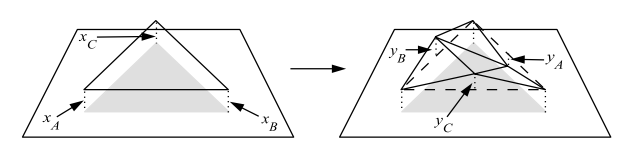
\includegraphics[width=\textwidth]{midpoint_displacement.png}
	\caption{\textit{A single iteration of midpoint displacement for the creation of mountains \cite{Prusinkiewicz1993}. New vertices $y_{A}$, $y_{B}$ and $y_{C}$ are created and shifted vertically by a random offset}}
	\label{fig:midpoint_displacement}
\end{figure}

To adapt this method to the generation of rivers on the terrain, rather than vertically displace newly formed triangle vertices, there edges are labelled as \textit{entry}, \textit{exit} or \textit{neutral} (figure \ref{fig:single_prod_of_midpoint_displacement}). An \textit{entry edge} defines the point of entry for the river into the triangle, an \textit{exit edge} the point of exit and a \textit{neutral edge} prevents the river from passing through. \\

When a production step is applied and a triangle split, the following constraints must be applied:
\begin{itemize}
\item An entry edge must split into an entry and a neutral edge.
\item An exit edge must split into an exit edge and a neutral edge.
\item A neutral edge must split into two neutral edges.
\item The newly formed edge-pairs within the triangle must either be "entry/exit" or "neutral/neutral".
\end{itemize}

\begin{figure}[h]
  \centering
	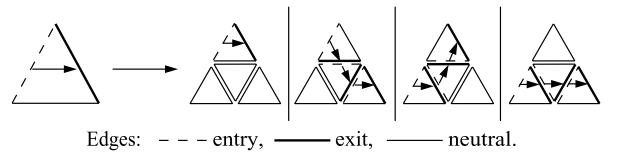
\includegraphics[width=\textwidth]{midpoint_displacement_for_rivers_1.png}
	\caption{\textit{Single production of midpoint displacement adapted to river generation \cite{Prusinkiewicz1993}. Given the initial triangle, four valid split scenarios.}}
	\label{fig:single_prod_of_midpoint_displacement}
\end{figure}

One difficulty with this technique is to ensure two adjacent triangles are coherent once split. That is, that the exit edge of one coincides with the entry edge of the other. To solve this, the location of edge vertices are used as the key to a random number generating hash table which, based on its output number, determines the segment that will be crossed by the river, if any.  \\

In their work, Génevaux et al. \cite{Genevaux2013} use fractal-based string rewriting to produce the river networks on the terrain. Once initial nodes have been selected to act as the river mouth, rewriting grammar is used to perform river node expansion. Configured values of $\rho_{a}, \rho_{s} and \rho_{c}$ influence the probability of selecting productions favouring asymmetric branching, symmetric branching and continuation without branching, respectively. The position for the new node is then selected based on the following constraints:
\begin{itemize}
\item It should be at a minimum distance from existing nodes and edges.
\item The new node should be at a greater distance from the terrain contour.
\item The new node should be compatible with the elevation constraints of existing nodes.
\end{itemize}
If a position satisfying these constraints is found, a new node is added at the given position and the process is repeated.\\

Both these techniques are successful in generating realistic river networks on terrains. The user, however, is limited in the amount of control he has over the resulting rivers. In the work by Génevaux et al. \cite{Genevaux2013}, for example, this is limited to specifying the preferred river branching behaviours. In terms of performance, Génevaux et al. \cite{Genevaux2013} are able to produce terrains of several hundred square kilometres in a matter of seconds.

\subsection{Explicit}

Explicit techniques use explicit input from the user to determine locations and properties of the river networks to generate.\\

Flood-filling is such a technique and is used in the work by Soon Tee \cite{Teoh2008} to permit users to place water reserves (e.g. sea, lakes, etc.) by clicking a single point on the terrain. This point which will act as the seed point for the water surface and will propagate iteratively to surrounding points at lower heights until all such points have been depleted. \\

Smelik et al. also use explicit techniques to create an interactive system permitting users to model a complete virtual world with content ranging from rural features (mountains, rivers, etc.) to man-made ones (buildings, road networks). When modelling the virtual world, interactions are split into two modes: \textbf{Landscape} and \textbf{Feature}. \textit{Landscape mode} permits the designer to paint ecotopes onto the terrain using traditional image editing tools. These ecotopes are predefined by the user and encompass both elevation and soil material information. In \textit{feature mode}, the user is able to place terrain content, including rivers. To do so, similarly to the interface provided by Emilien et al. \cite{Emilien2014}, the user sketches vector lines outlining the core path of the river and, based on this, a suitable course is plotted through the landscape. Other terrain features to which the river takes precedence adapt accordingly. For example, if the river is plotted to pass through a forest, trees on the rived bed and bank will be removed automatically. \\

Rather than placing vector-lines, the work by Soon Tee \cite{Teoh2008} and Št'Ava et al. \cite{StAva2008} permits users to click single points on the terrain which will act as the water source. The system then automatically generates a plausible path for the water down slope of the terrain.\\

As these methods provide very little automation in terms of guaranteeing consistency in the scene, the resulting realism is very much user-dependent. Real-time action-reaction feedback is essential with explicit modelling and so the majority of the methods run in real-time.

\subsection{Summary} \label{Summary}

Each technique has it's associated pros and cons and so choosing which one is best suited depends heavily on the requirements of the system. For example, if the terrain is fixed, using techniques which simulate real-time erosion of the terrain would be ill-suited. Similarly, if fine control over the resulting scene is necessary, heavily automated procedural methods which generate realistic scenes using very little user input would certainly not meet the requirements of the system. In this section we will summarize the pros and cons of the individual techniques in table form. These techniques will be rated based on:
\begin{itemize}
\item \textit{Automation}: The level of automation the technique provides.
\item \textit{Realism}: The realism of generated scenes.
\item \textit{Computational efficiency}: The techniques efficiency in terms of computational resources.
\item \textit{User-control}: How much control the user has over the final scene. 
\end{itemize}

\begin{table}[h]
  \centering
	    \begin{tabular}{|p{4cm}|p{3cm}|p{3cm}|p{3cm}|p{3cm}|}
  	    \hline	
  	      & \textbf{Automation} & \textbf{Realism} & \textbf{Computational Efficiency} & \textbf{User-control} \\
		\hline	
		\textbf{Classification-based} & 
		 %Automation  %Realism  %Comp. Effic. %User-control
		 Good  & Very Good  & Good & Very Good  \\
  	    \hline	
		\textbf{Fractal-based} & 
		 %Automation  %Realism  %Comp. Effic. % User-control
		 Excellent & Good & Good & Poor  \\
  	    \hline
		\textbf{Explicit} & 
		 %Automation  %Realism  %Comp. Effic. %User-control
		 Poor & Fair & Very Good & Excellent   \\
  	    \hline
  	    \multicolumn{5}{|c|}{\textbf{Simulation-based}} \\
  	    \hline				
  	    \textbf{Gravity} & 
		 %Automation  %Realism  %Comp. Effic. %User-control
		 Very Good & Good & Fair & Fair   \\
  	    \hline
		\textbf{Erosion} & 
		 %Automation  %Realism  %Comp. Effic. %User-control
		 Very Good & Very Good & Good & Fair      \\
  	    \hline
  	    	\textbf{Rainfall} & 
		 %Automation  %Realism  %Comp. Effic. %User-control
		 Very Good & Good & Good & Poor      \\
  	    \hline		
  	    \end{tabular}
  \caption{\textit{Summary of river placement techniques}}
	\label{Pros and cons of individual techniques}
\end{table}

In our system, the base terrain will take the form of a preloaded height map. Modifications to this terrain and modelling new terrains will be out-of-scope and, as such, all techniques which require such behaviour can be discarded.\\
Rainfall is a vital requirement to plant life and, as such, gathering rainfall data will be essential to model realistic vegetation on the terrain. Using this rainfall data along with soil properties, it is possible to calculate the amount of standing water which has not been absorbed by the soil. Using this, along with a gravitation simulation, it should be possible to determine main river networks on the terrain based on water builds up. The water drainage simulation employed here will be gravitational based and inspired from the hydrostatic pipe-model of Št'Ava et al. \cite{StAva2008}. It should be optimized to work in real-time and its duration controllable by the user in order to have fine-control over the size and depth of the resulting river networks (i.e. a longer simulation will drain more water and, as such, the river networks will be less intense).

\section{Vegetation}

Vegetation is core to rural landscapes. The species present along with their associated densities create a relationship between ecosystems and areas on earth on which resources are adequate. To ensure realism in virtual environments, much emphasize must be put on efficiently modelling these underlying ecosystems.\\

This section will review different methods to generate suitable vegetation for virtual worlds. These methods can be split into three main categories: \textit{Explicit Instancing, Probabilistic Instancing} and \textit{Plant Growth Modelling}.\\
\textit{Explicit Placement} require explicit user-input to directly or indirectly pinpoint exact locations for individual plant instances.\\
\textit{Probabilistic Placement} methods use statistical models to generate suitable vegetation.\\ 
\textit{Simulators} attempt to algorithmically reproduce plants battling for available resources.\\

We will measure the success of these techniques based on the level of automation they provide, the realism they achieve, their computational cost and their adaptability. Adaptability, here, represents the ease at which a given technique is able to model a number of different vegetation scenarios. \\

\subsection{Explicit Placement} \label{Explicit Placement}
Explicit placement methods require input from the user to determine the location and properties of individual plants. \\

Arnaud et al. \cite{Emilien} permit users to insert individual plants manually by simply clicking a given location on the terrain. To overcome the tedious task of manually placing individual plants on large terrains, the system is able to analyse existing distributions for reproduction. For example, to generate a large forest, the user is only required to generate a small subsection which can then be used to reproduce it on any scale (figure \ref{fig:explicit_placement_input_examplars}) \\

\begin{figure}[h]
  \centering
	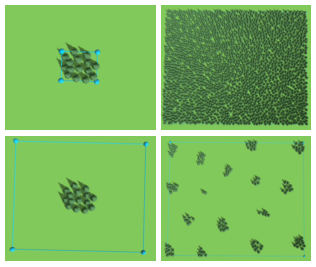
\includegraphics[natwidth=316,natheight=267]{worldbrush_forrest_reproduction.png}
	\caption{\textit{Using explicit placement as input examplars for reproduction \cite{Emilien}}}
	\label{fig:explicit_placement_input_examplars}
\end{figure}

Similarly, Deussen et al. \cite{Deussen1998} allow users to use grayscale raster images as input to specify terrain vegetation. The location of individual plants is determined by pixel location whereas plant properties are correlated to pixel intensity.\\

In their work focused on improving the realism of roadside landscapes, Andujar et al. ~\cite{Andujar2014} use orthophotos as input to determine the location and properties of individual plants. Unlike ordinary aerial photographs, aerial orthophotos use normalisation techniques to take into account terrain relief and camera tilt. The result is an image with uniform scale throughout which, similarly to a map, can be used to accurately measure distances between points. These orthophotos are used to measure the distances between plants. To later reproduce the roadside landscape, they use a dart throwing algorithm to place individual plants whilst respecting the measured distances. \\

\begin{figure}[!htb]
  \centering
	\label{Reconstructed roadside vegetation using orthophotos}
	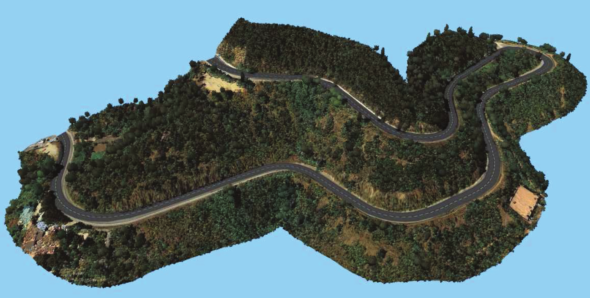
\includegraphics[width=\textwidth]{reconstructed_roadside_vegetation.png}
	\caption{\textit{Reconstructed roadside vegetation using orthophotos ~\cite{Andujar2014}}}
\end{figure}

Explicit placement methods provide significant user control over the resulting virtual world. However, as there is \textit{little to no automation} of this process, it can be very tedious and time consuming for the user. This is especially true when the virtual world being created are very large (e.g. open world video games). An advantage of this limited automation, however, is that modifications are most often very small and are therefore performed in real-time. \\
The \textit{adaptability} of these methods are very poor. Running a different scenario would most often involve starting the entire plant placement process again. \\
Creating vegetation for large virtual worlds using these methods is extremely strenuous and, as a consequence, realism is often compromised.

\subsection{Probabilistic Placement: Radial Distribution Analysis} \label{subsec:prob_placement_radial_dist}

Work by Emilien et al. \cite{Emilien}, Boudon et al. \cite{Boudon2007} and Lane et al. \cite{Lane2002} use radial distribution analysis to convert to metric form the underlying plant distributions of input examplars. The data generated by the analysis stage can later be used to synthesise, at any scale, new point distributions which respect the characteristics of the input exemplar. \\
For example, by analysing the positions of individual plants in a small subset of a forest and using it as the input exemplar, it is possible to reproduce it at a much larger scale in order to model its full size counterpart.\\

\paragraph{Analysis}

Generating the analytical data involves measuring the distances between individual points of different categories from the input examplar. For plant distribution analysis, the points represent individual plants and the categories represent the different species.\\

Before performing the analysis, the following parameters are configured:
\begin{itemize}
\item \textbf{R\textsubscript{min}}: The minimum distance from which point distances need to be analysed.\\
\item \textbf{R\textsubscript{max}}: The maximum distance after which point distances don't need to be analysed.\\
\item \textbf{Bin size}: When analysing the distances of given points, it is necessary to aggregate the points which reside at similar distances into bins. The bin size is the range represented by a single bin.\\
\end{itemize}

A core part of radial distribution analysis is generating pair correlation histograms for each category pair combination. A pair correlation histogram \textit{H\textsubscript{AB}} represents the variation in the distance between points of of category \textit{C\textsubscript{A}} and \textit{C\textsubscript{B}} ranging from \textit{R\textsubscript{min}} to \textit{R\textsubscript{max}} in \textit{bin size} increments (figure \ref{fig:pair_correlation_histograms}) \\

\begin{figure}[h]
  \centering
	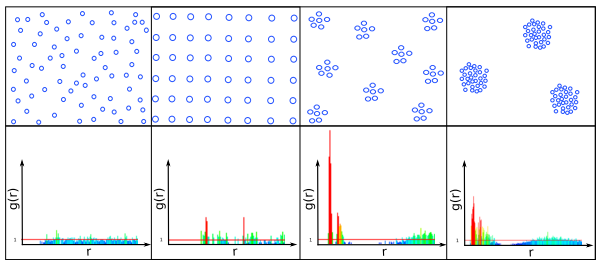
\includegraphics[width=\textwidth]{pair_correlation_histograms.png}
	\caption{\textit{Point distributions with associated pair correlation histogram \cite{Emilien2014}}}
	\label{fig:pair_correlation_histograms}
\end{figure}

To generate the pair correlation histogram \textit{H\textsubscript{AB}}, the algorithm iterates through each reference point of category \textit{C\textsubscript{A}} and, for each destination point of category \textit{C\textsubscript{B}} at a distance between \textit{R\textsubscript{min}} and \textit{R\textsubscript{max}}, increments the relevant bin in the histogram. In figure \ref{fig:radial_distribution_analysis_example}, for example, are being measured the points that lie within the annular shell of radius \textit{r} with bin size \textit{d\textsubscript{r}} (area \textit{d\textsubscript{A}}). 

\begin{figure}[h]
  \centering
	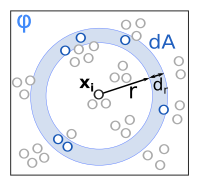
\includegraphics[natwidth=199,natheight=140]{radial_distribution_analysis.png}
	\caption{\textit{Radial distribution analysis}}
	\label{fig:radial_distribution_analysis_example}
\end{figure}

Because of their larger circumference, the coverage area of annular shells get larger as the distance bin being measured increases. In other words, \textit{A\textsubscript{r}} \textless \textit{A\textsubscript{r+1}} where \textit{A\textsubscript{r}} is the area covered by the annular shell starting at distance \textit{r}. A direct consequence of this is that annular shells at further distances will naturally be prone to containing more points. To counter for this, normalisation is performed based on annular shell area. \\

The radial distribution analysis function \textit{h\textsubscript{rdf}} is as follows:\\
\begin{center}	
$h_{rdf}(k) = \sum_{x_{i} \in X} \sum_{y_{j} \in Y \&  
kd_{r} \leq d(x_{i}, y_{j}) < (k+1)d_{r} } \frac{A}{d_{A}n_{x}n_{y}} $
\end{center}
Where:
\begin{itemize}
\item \textit{hrdf(k)} is the k-th value of the pair wise histogram.
\item \textit{X} are the points of category X (reference points).
\item \textit{Y} are the points of category Y (target points)    .
\item \textit{d\textsubscript{r}} is the annular shell width.
\item \textit{A} is the total analysed area.
\item \textit{n\textsubscript{x}} and \textit{n\textsubscript{y}} are the number of points of categories \textit{x} and \textit{y} respectively. Note that pairwise histograms also need to be calculated for points of the same category. In this situation, category \textit{x} and category \textit{y} would be the same.
\item \textit{d\textsubscript{A}} is the area of the annular shell being analysed.
\end{itemize}

Conceptually, this formula calculates the variance from the average density of the target category at incremental distances from points of the reference category.\\

\paragraph{Reproduction}

In order to reproduce the distribution of the input exemplar, points are added iteratively whilst matching as closely as possible the corresponding pair correlation histogram data calculated during the analysis stage. Metropolis-Hastings sampling ~\cite{Hurtut2009} is the most common way to do this. It involves performing a fixed number of point birth-and-death perturbations. A change from the initial arrangement \textit{X} to the new arrangement \textit{X'} is accepted with probability \textit{R}, where:

\begin{center}
$ R = \frac{f(X')}{f(X}$
\end{center}
\textit{f(X)} is the probability density function (PDF) of a given arrangement and is expressed as:\\

\begin{center}
$ f(X) = \prod_{C_{Y_{K}} \leq C_{X}} 
		 \prod_{x_{i} \in X}
		 \prod_{y_{i} \in Y_{k}} 
		 h_{X,Y_{k}}(d(x_{i},y_{j}))$
\end{center} 

Where:
\begin{itemize}
\item \textit{C\textsubscript{y}} and \textit{C\textsubscript{x}} represent categories \textit{Y} and \textit{X}, respectively.
\item \textit{X} are all points of category \textit{X}.
\item \textit{Y} are all points of category \textit{Y}.
\item h\textsubscript{X,Y\textsubscript{k}}(d(x\textsubscript{i}, y\textsubscript{j})) is the value retrieved from the pairwise histogram of categories \textit{X} and \textit{Y} given the distance between points \textit{x\textsubscript{i}} and \textit{y\textsubscript{i}}.
\end{itemize}
Intuitively, the PDF defines, given a set of points, the aggregate strength of the current distribution.\\

Because the PDF formula is a product, calculating it for a new layout \textit{X'} with appended/removed point \textit{P} only involves calculating the PDF for the single reference point \textit{P}. As a consequence, reproduction can be performed very efficiently. In their work, Emilien and Cani ~\cite{Emilien} are able to perform analysis and reproduction in near real-time.\\

When using this technique to reproduce a plausible plant distribution, Boudon et al. \cite{Boudon2007} take it one step further by enabling plant crowns to deform based on predefined elasticity parameters. Because the crowns are not constrained to being circular, they can deform to facilitate the survival of plants at a lower height.

\subsection{Probabilistic Placement: Predefined Ecosystems}

In their work, Hammes el al. \cite{Hammes2001} predefine ecosystems along with their preferred environment. These environments are defined in terms of:

\begin{itemize}
\item Elevation: All plant species have an upper limit after which temperature or oxygen levels are ill-suited.
\item Relative elevation: The local changes in height. Local minimums tend to be valleys and therefore wetter with less illumination. Local maximums, on the other hand, tend to me ridges which are dryer and much more exposed.
\item Slope: Gradient has a direct impact on the quality of the soil and therefore the plants which can grow. When slopes get steeper, plants tend to get much smaller as they struggle to get required nutrients from the soil.
\item Slope direction: This has a direct effect on sunlight exposure. Southern facing slopes in the northern hemisphere will have a greater exposure to the sun and vice-versa for the southern hemisphere.  
\end{itemize}

All these ecosystems are stored in a database and, when vegetation is to be placed on the terrain, the most suitable ecosystems are chosen based on the terrain properties mentioned above. See figure \ref{fig:vegetation_generated_using_predefined_ecosystems} for an example landscape generated using this technique.

\begin{figure}[h]
  \centering
	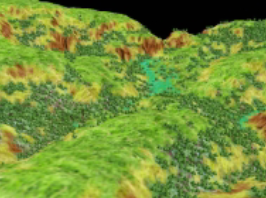
\includegraphics{predefined_ecosystems.png}
	\caption{\textit{Vegetation generated using predefined ecosystems \cite{Hammes2001}}}
	\label{fig:vegetation_generated_using_predefined_ecosystems}
\end{figure}

\subsection{Probabilistic Placement: Conclusions}

\textit{Probabilistic Placement} permit users to specify only small portions of input data to populate large areas. For the \textit{Radial Distribution Analysis} approach, this input data would be in the form of an input distribution. For the \textit{Predefined Ecosystems} approach, it would be a predefined ecosystem along with its preferred environment. Although this automation does ease the task for artists, specifying accurate input data is still crucial to produce realistic vegetation. Consequently, although the realism achieved by these methods is generally good, their adaptability is still limited. \\
Thanks to the use of efficient algorithms, the computational complexity of these methods are often low and real-time updating is achievable. 

\subsection{Simulators: Plant Growth Modelling} \label{subsec:simulators_plant_growth_modelers}

Plant growth modeller attempt to algorithmically reproduce the laws of nature with such precision that they can be used in agronomical sciences and forestry to estimate and maximize crop yield. To achieve this, such simulators go into great detail to model the available resources. For example,  work by Soler et al. ~\cite{Soler2001,Soler2003} splits single plants into geometrical organs with unique light transmittance and reflectance properties. By doing so, light propagation within the plant can be simulated in order to determine the aggregated photosynthetic potential. This work, along with that of Yan et al. ~\cite{Yan2004}, base their simulators on two vital and widely accepted laws of nature:
\begin{itemize}
\item \textit{Law of the sum of temperatures}: Plants grow in cycles which vary from days to years depending on the specie. The law of the sum of temperatures states that the frequency of these cycles is proportional to the sum of the daily average of the temperatures.
\item \textit{Law of the water use efficiency}: The amount of fresh matter fabricated by a plant is proportional to the water evaporation of the plant. This factor is called the water use efficiency. 
\end{itemize}

Water evaporates during photosynthesis as the plant exchanges water for carbon dioxide. Based on this and the law of water use efficiency outlined above, the amount of fresh matter produced (i.e growth) for a given plant is directly correlated to the amount of photosynthesis performed. Using this, Soler et al. ~\cite{Soler2001} apply the following formula to calculate the amount of fresh matter, \textit{Q\textsubscript{m}(t)}, created by a given plant at time \textit{t}:\\

\begin{center}	
\textit{$Q_{m}(t)$} = $\sum_{x=1}^{N(t)} \frac{E(x,t)}{R} $
\end{center}
Where:
\begin{itemize}
\item \textit{E(x,t)} is the potential for matter production of the \textit{x}-th leaf at the \textit{t}-th cycle. It is proportional to the incoming radiant energy up to a certain threshold, after which it remains constant. 
\item \textit{R} is the hydraulic resistance of the given leaf. This resistance is what limits water evaporation (photosynthesis) and therefore growth. It varies depending in the species and surface area.
\end{itemize} 
Intuitively, this formula calculates the total available fresh matter, \textit{$Q_{m}$}, that can be produced for an individual plant \textit{P} at a given time \textit{t}, by calculating the photosynthesis potential of each individual leaf of \textit{P} given the current lighting.\\

Using this, the algorithm iterates through growth cycles with a frequency that is calculated based on the \textit{law of the sum of temperatures} mentioned above. Each growth cycle performs the following two steps:
\begin{enumerate}
\item The lighting and therefore photosynthesis potential of each individual leaf of the plant is calculated. This is then used to calculate, as above, the quantity of fresh matter produced.
\item The fresh matter is then distributed to different organs of the plant according to an associated organ strength.
\end{enumerate}

By going into such detail, these simulators produce very realistic simulations of the evolution of plants. For example, to maximize growth, plants are able to grow in direction of the light source (figure \ref{fig:plant_growing_towards_light_source}).\\

\begin{figure}[h]
  \centering
	    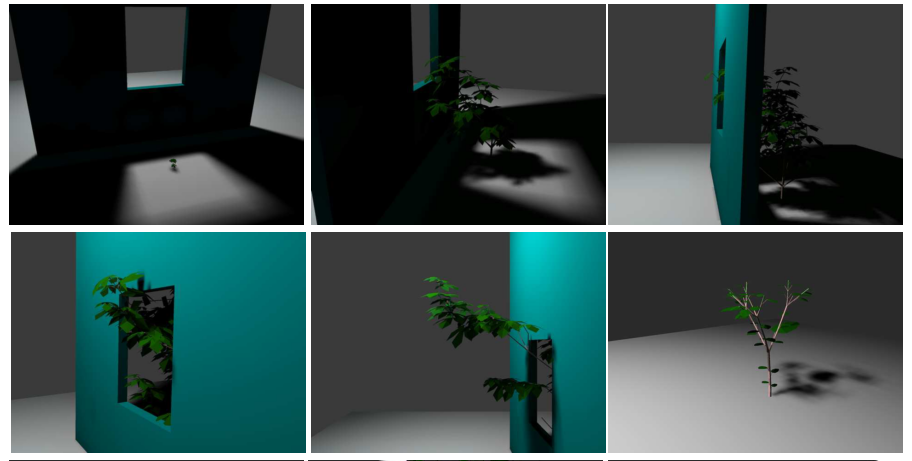
\includegraphics[width=\textwidth]{plant_growing_towards_light_source.png}
	\caption{\textit{Plant growing towards light source ~\cite{Soler2001}}}
	\label{fig:plant_growing_towards_light_source}
\end{figure}

\subsection{Simulators: Ecosystem Simulators} 

Ecosystem simulators use procedural methods to algorithmically reproduce the competition for resources that occurs in nature during plant growth. In nature, this competition is an extremely complex process and so reproducing it exactly would be infeasible. Instead, a simplified model of this ecological process is implemented. During these simulations, available resources fluctuate and each plants strength is continuously recalculated based on its associated properties. This strength directly affects the plants growth and chance of survival. \\
Such plant properties include: age; vigor; shade tolerance; humidity requirement and temperature requirements. Amongst others, the resources modelled include: available illumination; available humidity; temperature and slope.

The aim of ecosystem simulators is to determine, given an initial state \textbf{\textit{S\textsubscript{t}}} of the system at time \textbf{\textit{t}} and a simulation time \textbf{\textit{n}}, the state \textbf{\textit{S\textsubscript{t+n}}}. \\
The state of the system represents individual plant instances with associated location and properties. \\

Lindenmayer systems, commonly referred to as L-systems, use a formal grammar along with a set of production rules to iteratively create larger strings from a starting string called the axiom. Such systems are commonly used to model plants and plant growth ~\cite{Prusinkiewicz1990,Deussen2002,Boudon2012,Prusinkiewicz1993}. \\
An extension to basic L-systems, referred to as open L-systems, adds a communication grammar which permits the set of production rules to behave differently depending on predefined conditions ~\cite{Prusinkiewicz1996}. In their work modelling the growth of struce trees, Berezovskava et al. \cite{Berezovskava1997} use different production rules depending on local bud density. This is a simplified representation of buds competing for available light. \\

By introduction multiset L-Systems, Lane and Przemyslaw ~\cite{Lane2002} extend L-systems yet further to model an ecosystem simulator. The production rules for multiset L-systems work in two stages. The first, identical to basic L-Systems, produces a new string given an input string and production rule. The second, splits the resulting string into new sets using a predefined separation symbol. In their work, the different sets represent different plant instances, thus enabling new plants to spawn during the production steps. When building their L-System, Lane and Przemyslaw ~\cite{Lane2002} focus on reproducing three important properties of nature, each distinctly testable to determine the plausibility of the results:
\begin{itemize}
\item \textit{Self-thinning}: When plants grow, their resource requirements increase and, as a direct consequence, inter-plant competition for resources increases. Eventually, the competition becomes too intense and resources too scarce leading to more vigorous plants starving smaller plants. At this point, self thinning begins and plant densities decrease.
\item \textit{Succession}: Given plant species \textit{A} with a fast growth rate and species \textit{B} with a slower growth rate but higher shade tolerance. At first, the faster growing species \textit{A} will dominate and flourish but, with time, the slower growing but more shade tolerant species \textit{B} will flourish and dominate.
\item \textit{Propagation}: Plants often propagate in clusters surrounding the seeding plant.
\end{itemize}

The L-System they implemented contains different production rules to represent the different properties of nature mentioned above. A single simulation and the corresponding output can be seen in figure ~\ref{fig:plant_placement_using_an_ecosystem_simulator_modelled_by_L_system}.

\begin{figure}[h]
  \centering
    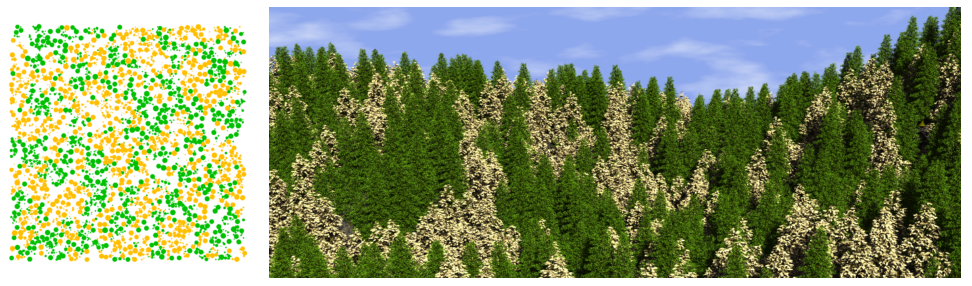
\includegraphics[width=\textwidth]{L-System-Result.png}
    \caption{ \textit{Plant placement using an ecosystem simulator modelled by L-Systems ~\cite{Lane2002}. \textit{Left:} Result of the simulation where orange circles indicate the positions of poplar trees and green circles the positions of spruce trees. \textit{Right:} Reproduced virtual world where the location of individual plants is deduced from the output of the simulator.}}
    \label{fig:plant_placement_using_an_ecosystem_simulator_modelled_by_L_system}
\end{figure}

Work by Deussen et al. ~\cite{Deussen1998} also uses L-Systems as the basis for an ecosystem simulator. As an extension to the work by Lane and Przemyslaw ~\cite{Lane2002}, they introduce the notion of soil humidity and an associated soil per species humidity preference.

A direct consequence of the automation provided by these ecosystems is that fine control over the final vegetation content is lost. Deussen et al. ~\cite{Deussen1998} overcome this, however, by offering a hybrid approach where the ecosystem simulator is first used to populate the entire terrain and explicit instancing is used thereafter for the detailing .\\

Another weakness of procedural ecosystems based on L-Systems worth mentioning is that the communication parameter is binary; in the work by Lane et al. ~\cite{Lane2002} a plant will be dominated as soon as it’s radius intersects another larger plant, at which point it will die with a set probability. This probability of death will stay constant and will not increase as this domination increases. Similarly, in the humidity model of Deussen et al. ~\cite{Deussen1998}, a plant has a preference for wet or dry areas and there is no notion of a measurable humidity preference range. This could prove problematic to model species which are able to adapt to a multitude of environments with varying resource availability (e.g. grass). \\

\subsection{Simulators: Conclusions}
Probably the main advantage of simulators over other approaches is the level of \textit{automation}. Running simulations is done with easy and requires very little input from the user. \\
Although the adaptability of these methods is also impressive, it is limited by the necessity to configure the properties for individual species. This is especially true for \textit{Plant Growth Modelling} approaches where topological data must be configured. Obtaining topological data often involves real-world analysis of the plants growth cycles. \\
Computational cost is often high when using simulators. The extent of which is dependant on the level of detail and the number of plants being simulated simultaneously. For example, in the highly detailed simulations of Soler et al. ~\cite{Soler2001}, simulating 45 cycles for a single plant takes approximately 15 minutes.\\

\subsection{Summary} \label{subsec:vegetation_summary}

Which technique (Explicit, Probabilistic or Simulators) to use entirely depends on the requirements of the system. For example, if realism is the key priority then ecosystem simulators able to provide botanical realism would be the most suitable approach. Choosing the technique is therefore all about minimizing the associated compromises. In table \ref{tab:pros_and_cons_of_vegetation_placement_techniques} we summarize the pros and cons of the individual techniques based on the following criteria: 
\begin{itemize}
\item \textit{Automation}: The level of automation the technique provides. That is, how little user input is needed.
\item \textit{Realism}: The level of realism with which the technique models real-world ecosystems.
\item \textit{Computational efficiency}: The techniques efficiency in terms of computational resource requirements.
\item \textit{Adaptability}: How well the technique can adapt to model different scenarios.
\end{itemize}

\begin{table}[h]
  \centering
	    \begin{tabular}{|p{4cm}|p{3cm}|p{3cm}|p{3cm}|p{3cm}|}
  	    \hline	
  	      & \textbf{Automation} & \textbf{Realism} & \textbf{Computational Efficiency} & \textbf{Adaptability} \\
		\hline	
		\textbf{Explicit Placement} & 
		 %Automation  %Realism  %Comp. Effic. %Adaptability
		 Poor  & Poor  & Excellent & Poor      \\
  	    \hline	
  	    \multicolumn{5}{|c|}{\textbf{Probabilistic Placement}} \\
  	    \hline				
  	    \textbf{Radial Distribution Analysis} & 
		 %Automation  %Realism  %Comp. Effic. %Adaptability
		 Good & Very Good & Very Good & Fair   \\
  	    \hline
		\textbf{Predefined Ecosystems} & 
		 %Automation  %Realism  %Comp. Effic. %Adaptability
		 Good & Fair & Very Good & Poor      \\
  	    \hline
		\multicolumn{5}{|c|}{\textbf{Simulators}} \\
  	    \hline		
		\textbf{Plant Growth Modelling} & 
		 %Automation  %Realism  %Comp. Effic. % Adaptability
		 Excellent & Excellent & Poor & Fair  \\
  	    \hline
		\textbf{Ecosystem Simulators} & 
		 %Automation  %Realism  %Comp. Effic. %Adaptability
		 Excellent & Very Good & Fair & Good   \\
  	    \hline
  	    \end{tabular}
  \caption{\textit{Summary of vegetation placement techniques}}
  \label{tab:pros_and_cons_of_vegetation_placement_techniques}
\end{table}

Given a set of plant species, available resources and terrain, our system must be able to specify the locations of individual plants. The output must be: visually realistic; easily scalable in order to be able to re-run simulations with different input species; computationally efficient to ensure the effect of user actions appear in close to real-time. \\
Given these requirements, a hybrid approach is best suited which combines the adaptability and realism of ecosystem simulators with the computational efficiency of probabilistic placement. Computationally expensive ecosystem simulator runs will be performed beforehand in order to acquire the necessary distribution data. This data will then be stored in order for it to be queried at a later stage without having to redo expensive simulations. When placing vegetation in the virtual world, pre-calculated distribution data will be queried and probabilistic instancing used to fill user-defined areas with suited plant species and realistic distributions. \\

\chapter{System Overview}

\begin{figure}
\center
	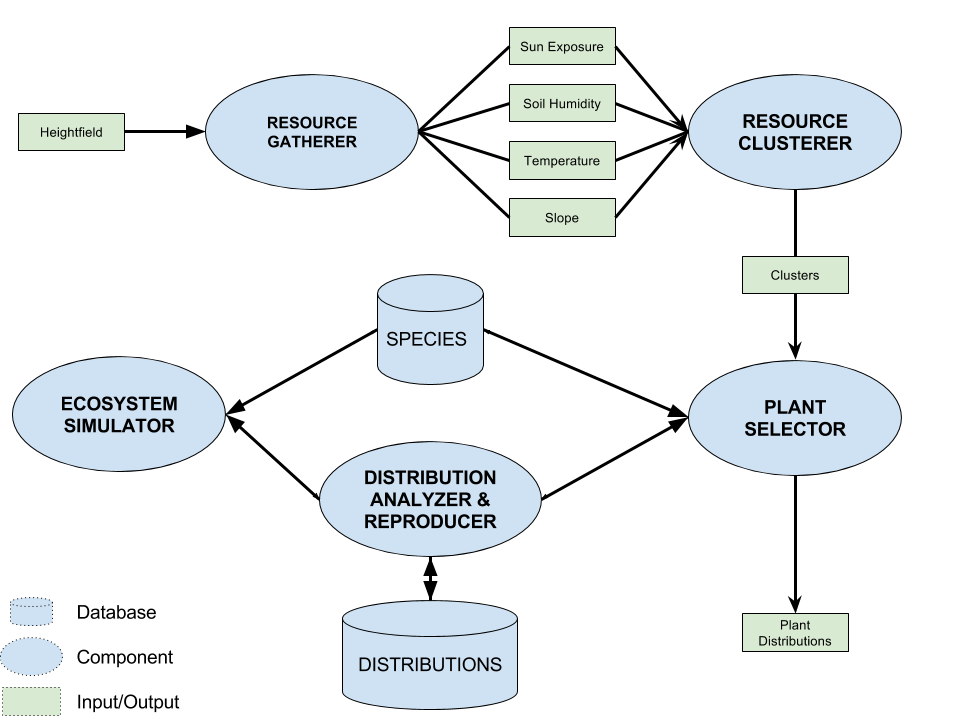
\includegraphics[width=\textwidth]{system_overview.png}
	\caption{ System overview}	
	\label{fig:system_overview}
\end{figure}

Multiple components serving specific purposes constitute the building blocks of the overall system, notably: \textit{resource gathering}, \textit{resource clustering}, \textit{plant selection}, \textit{ecosystem simulation} and \textit{distribution analysis and reproduction}. The purpose of this chapter is to give an overview of the system, each component and how they fit together (as illustrated in figure \ref{fig:system_overview}). To do so, an overview of each component is provided separately along with it's purpose, required inputs and outputs. To conclude this chapter, the \textit{limitations} of the system will be discussed. \\

\section{Resource Gatherer}

Vegetation requires resources to grow and the distribution of these resources identifies a given species and associated it with a given climate and, subsequently, location on earth. Determining resource data is essential, therefore, to generating realistic virtual worlds as it is vital to determining vegetation distribution patterns. The purpose of the resource gatherer is to determine, for each terrain vertex: \textit{sun exposure}, \textit{soil humidity}, \textit{temperature} and \textit{slope}. Figure \ref{fig:system_overview_resource_gatherer} illustrates the output of the resource gatherer along with the user inputs required.\\
The latitude and orientation of the terrain must be specified by the user in order to determine the sun position throughout the year. The \textit{sunlight exposure} calculation then determines, given this information and the terrain relief, the average daily illumination (in hours) received by each terrain vertex for each month of the year. To calculate the average illumination for a given month, the trajectory of the sun is calculated for the fifteenth day. \\
In order to calculate the \textit{soil humidity} for each month, the soil infiltration rate, monthly rainfall quantity and monthly rainfall intensity must be configured.\\
To determine the \textit{temperature} of each terrain vertex, the user must specify the temperature at zero metres in June and December along with the associated lapse rate. These temperatures are then considered the annual minimum and maximum and are used to deduce the temperature for any month through linear interpolation. The lapse rate represents the decrease in temperature with altitude and is used to determine the temperature for any terrain vertex given its altitude. \\
The \textit{slope} is determined automatically from the input terrain.\\

\begin{figure}
\center
	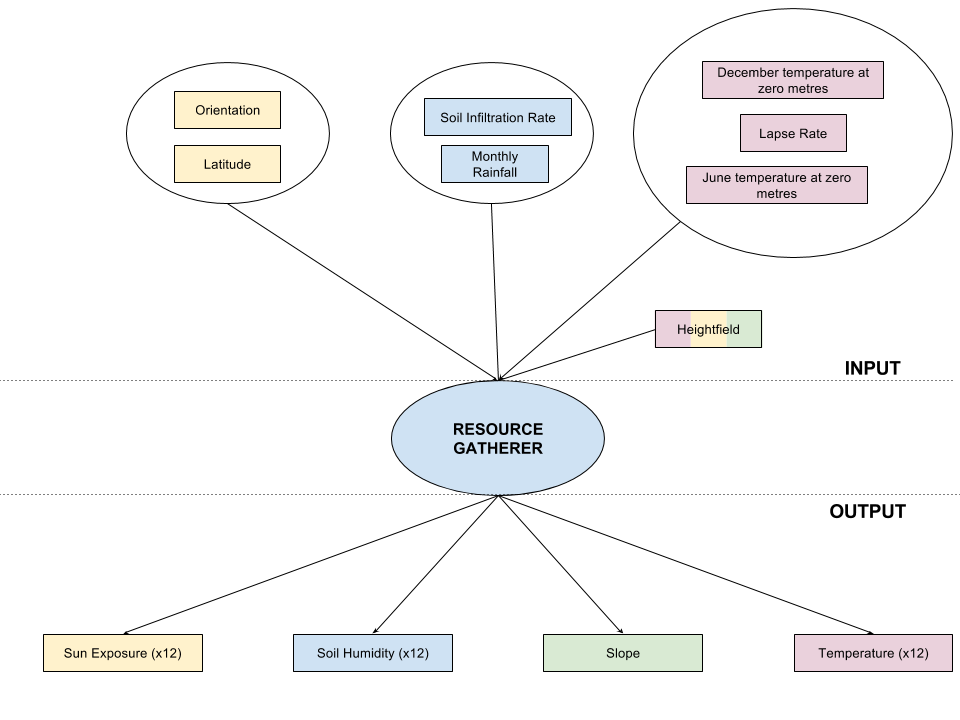
\includegraphics[scale=0.3]{system_overview_resource_gatherer.png}
	\caption{ Resource gatherer overview with colour coding to correlate input with corresponding output.}	
	\label{fig:system_overview_resource_gatherer}
\end{figure}

\section{Resource Clusterer}

Determining a suitable plant distribution for each individual terrain vertex is infeasible due to the associated computational cost. To reduce the amount of plant distributions to calculate, K-means clustering is performed on the terrain to group together points with similar resource properties. The mean value of each cluster is then used to determine suitable vegetation and distribution thereof. Figure \ref{fig:system_overview_resoure_clusterer} illustrates the input requirements and output of this component.

\begin{figure}
\center
	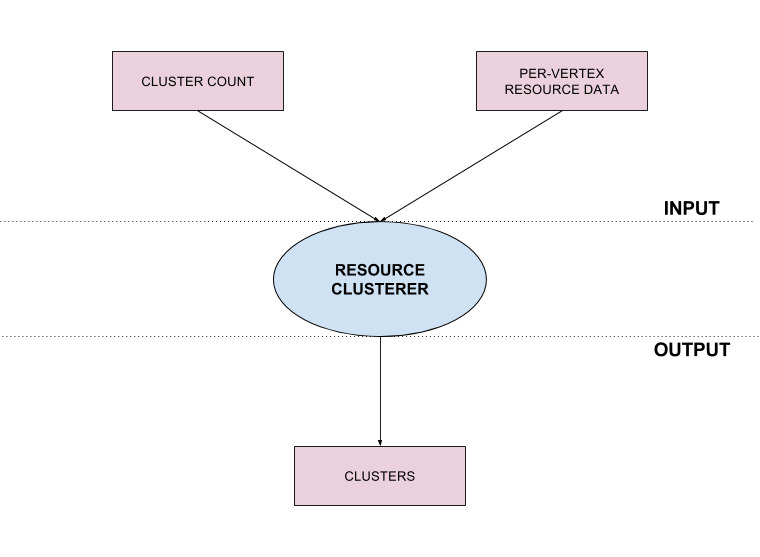
\includegraphics[scale=0.3]{system_overview_resource_clusterer.png}
	\caption{ Resource clusterer overview.}	
	\label{fig:system_overview_resoure_clusterer}
\end{figure}

\section{Plant Selector}

Given the mean value of the individual clusters, the plant selector determines the plants which are able to survive in each terrain cluster and calculates for each of them a suitability score. This score depicts how suited a specie is to each individual cluster and is illustrated to the user for informational purposes in order to facilitate the specie selection procedure. Figure \ref{fig:system_overview_plant_selector} shows the input requirements and outputs of this component.

\begin{figure}
\center
	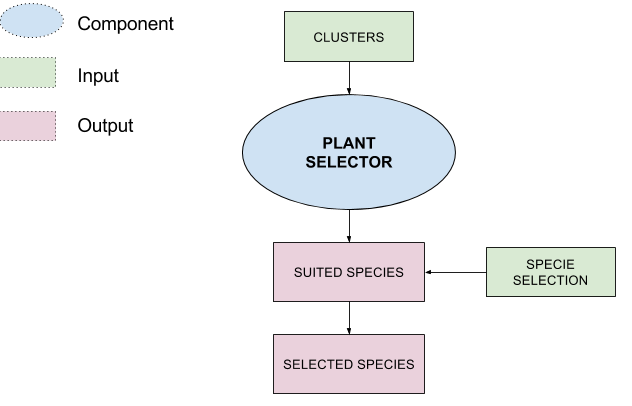
\includegraphics[scale=0.3]{system_overview_plant_selector.png}
	\caption{ Plant selector overview.}	
	\label{fig:system_overview_plant_selector}
\end{figure}

\section{Ecosystem Simulator}

The ecosystem simulator is used to determine a valid plant distribution given a set of plant species and resources (soil humidity, illumination, slope and temperature). To do so, it simulates plants spawning, growing, battling and dying through time at monthly intervals on a hundred by hundred metre simulation area. Figure \ref{fig:system_overview_ecosystem_simulator} shows the input requirements and outputs of this component.

\begin{figure}
\center
	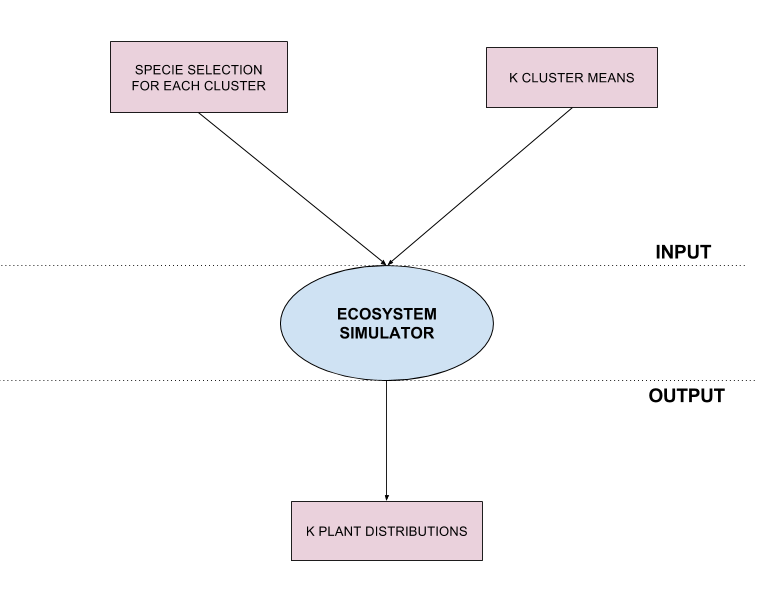
\includegraphics[scale=0.3]{system_overview_ecosystem_simulator.png}
	\caption{ Ecosystem simulator overview.}	
	\label{fig:system_overview_ecosystem_simulator}
\end{figure}

\section{Distribution Analyser and Reproducer}

Because the ecosystem simulator is computationally expensive, the simulation area is restricted to ten thousand square metres (hundred by hundred metres). In order to place vegetation in clusters with larger surface areas, radial distribution analysis and reproduction is performed. This technique analyses the variation in plant density over distance of an input exemplar in order to generate pair correlation histograms which are used to reproduce distributions matching the characteristics of the input exemplar. Because the reproduction is much less computationally costly than the ecosystem simulator, it is possible to efficiently produce distributions covering much larger areas. Figure \ref{fig:system_overview_distribution_analyser_and_reproducer} shows the input requirements and outputs of this component.

\begin{figure}
\center
	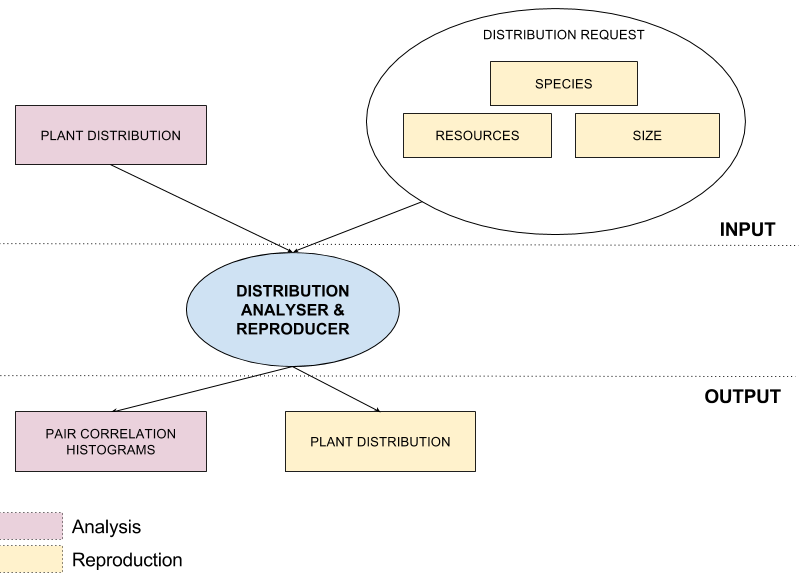
\includegraphics[scale=0.3]{system_overview_radial_distribution_analyzer_and_reproducer.png}
	\caption{ Distribution analyser and reproducer overview.}	
	\label{fig:system_overview_distribution_analyser_and_reproducer}
\end{figure}

\chapter{Terrain and Resources} \label{chap:terrain_and_resources}

The first step in creating virtual worlds is specifying the base terrain on which features will be placed. Subsequently, terrain resources with direct influence on content are determined. In order to strike a good balance between resulting realism and user experience, procedural methods must be employed when suited.\\
This chapter discusses how a system fitting these requirements was built. The discussion is split into the following core sections: \textit{Terrain \& Navigation}, \textit{Resources}, \textit{Rivers \& Streams}, \textit{Water Reserves} and \textit{Results}.\\
\textit{Terrain \& Navigation} discusses how the base terrain is selected and navigated through. \\
In order to determine suitable vegetation and river sources, resource data needs to be specified. How this is done is discussed in the \textit{Resources} section.\\
Essential to the realism of virtual terrains is water placement. This water can take the form of rivers and streams or water reserves. Techniques used to place such content are discussed in the \textit{Rivers and Streams} and \textit{Water bodies} sections, respectively. \\


\section{Terrain and Navigation}

In order to give the user the freedom to model any type of virtual world, providing the ability to specify any type of base terrain is essential. Efficiently rendering and navigating this terrain is also key for both the user experience and visual realism. How our system manages these requirements are discussed sections \textit{Loading Terrain}, \textit{Rendering Terrain} and \textit{Navigating Terrain} below.

\subsection{Loading Terrain}

As stated previously, our work focuses on terrain content and not terrain relief modelling. As such, the user is only able to load a static, pre-generated terrain in the form of a Terragen height-map. A height-map is a 2-dimensional grid of height values which, once loaded and converted, represents the height of the terrain on a regular grid. The Terragen file format is a freely available and widely used file-specification created by PlanetSide \protect\footnotemark \footnotetext{\url{http://www.planetside.co.uk}} for their realistic virtual world generation software, Terragen. The format wraps raw height data with other important information essential to accurate rendering such as base height, scales and dimensions.\\
Note that modelling the base terrain as static is a simplification as in reality it is affected by erosion. The extent of which depends on many factors including wind, vegetation and water.

\subsection{Rendering Terrain}

Once parsed, the height-map data is transferred to the GPU as a two dimensional texture for rendering. In order to better visualize the terrain relief, a Blinn–Phong shading model is used when rendering the terrain.
This shading model takes into consideration camera viewpoint and lighting incidence angles to determine the influence of diffuse and specular lighting on individual terrain vertices. This information is subsequently used to calculate a weighted contribution of ambient, specular and diffuse colors to determine the aggregate color of individual terrain vertices. By accurately modelling specular and diffuse highlights, renders are more realistic and shapes more distinguishable \citep{Blinn}. By employing this model in this work, terrain relief is made clear.\\
Essential to the Blinn-Phong shading model are the normal vectors for each terrain vertex. This is done using the algorithm outlined in equation \ref{eq:normals_calculation} and illustrated in figure \ref{fig:normals_calculation}. Each normal is calculated in parallel on the GPU, thus ensuring real-time results.

\begin{equation} \label{eq:normals_calculation}
N_{P} = V_{ac} \times V_{db}
\end{equation}
Where: $N_{P}$ is the normal vector at point P and $P_{A}$, $P_{B}$, $P_{C}$ and $P_{D}$ are the direct points surrounding P in the X and Y direction (see figure \ref{fig:normals_calculation}).

\begin{figure}[h]
\center
	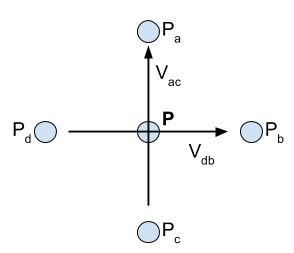
\includegraphics[width=\textwidth/2]{normals_calculation.png}
	\caption{Illustration of the vertices and vectors used to calculate terrain normal at position \textit{P}.}
	\label{fig:normals_calculation}
\end{figure}

\subsection{Navigation}

In order for users to successfully and intuitively navigate through virtual worlds, it is important to prevent disorientation by ensuring continuous user awareness of location and orientation \cite{Darken1993}. 
In their work, Darken et al. \cite{Darken1993} explore various navigation techniques to do so, including the flying scenario where users explore virtual worlds as if they were flying through it. This navigation technique provides a birds eye view of the virtual worlds and enables users to gain an overview of the terrain and efficiently locate landmarks to serve as point of references. Locating such landmarks proves extremely useful in keeping the user aware of his location and therefore preventing disorientation \cite{Darken1993}. Birds eye has become the most widespread navigation technique employed in video games, simulators and virtual world generation software. In order to support a variety of users (novice to computer graphic experts), this is the navigation style used in our system. To further prevent disorientation, a compass is continuously displayed stating the current heading. \\

Intuitive controls and suitable sensitivity thereof are also essential. The correlation between key-press and mouse movement must be predictable so that the user can navigate in three dimensional space without losing his bearings. In an attempt to cater for the control requirements of a wider user-base, two different control types are available in this system: \textit{keyboard-driven} and \textit{click-and-drag}. Details of which can be found in table \ref{tab:control_types}. The active control type is easily configurable, along with sensitivity parameters, through the application's configuration interface.

\begin{table}[h]	
  \centering
	    \begin{tabular}{|p{2.5cm}|p{2.25cm}|p{2.25cm}|p{2.25cm}|p{2.25cm}|p{2.25cm}|}
  	    \hline	
  	    \textbf{Control-type} & \textbf{Translate Left/Right} & \textbf{Translate Up/Down} & \textbf{Translate Front/Back} & \textbf{Rotate Left/Right} & \textbf{Rotate Up/Down} \\
		\hline
		\textbf{First-Person} & A/D key-press & - & W/S key-press & Horizontal mouse movement & Vertical mouse movement \\
		\hline
		\textbf{Click-and-drag} & Horizontal click \& drag & Vertical click \& drag & Scroll wheel & Ctrl + horizontal click \& drag & Ctrl + vertical click \& drag\\
		\hline
		\end{tabular}
		\caption{Control types instruction sheet}
		\label{tab:control_types}
\end{table}


\section{Resources}

\section{Rivers \& Streams}

Essential to the realism of virtual rural terrains are water networks which take the form of rivers and streams. These rivers form as run-off water is being transported by gravity from higher to lower grounds. In this section is  The algorithm used to model gravity and therefore the evacuation of water on any terrain is outlined below along with details on the GPU implementation used to accelerate the process.

\subsection{Water Evacuation Algorithm} 

Precipitation, precipitation intensity and soil infiltration are used to calculate the soil humidity, $S_{h}$, which equates to the quantity of water, in millimetres, absorbed by the soil. The water which isn't absorbed by the soil, \textit{W$_{standing}$} for a given terrain vertex can therefore be deduced using equation \ref{eq:standing_water_calculation}

\begin{equation} \label{eq:standing_water_calculation}
	W_{standing} = R_{q} - S_{h}
\end{equation}
where:
\begin{itemize}
\item \textit{W$_{standing}$} is the standing water, in millimetres.\\
\item \textit{R$_{q}$} is the monthly rainfall quantity, in millimetres.\\
\item \textit{S$_{h}$} is the quantity of water absorbed by the soil, in millimetres.\\
\end{itemize}

Similarly to the work by Stava et al. \cite{StAva2008}, a water evacuation algorithm is used where water is iteratively evacuated from source to destination vertices.

\subsection{GPU Implementation}

through the evacuation of run-off water from higher to lower altitudes and, eventually, 

Water networks form due to the evacuation of 

\section{Water Bodies} \label{sec:water_bodies}

Water bodies refers here to static water build-ups such as seas, oceans and lakes. The water-flow simulation \label{sec:rivers_and_streams} often fails to reproduce these accurately as they are the result of years of water accumulation, groundwater and different soil infiltration rates. Users can place such water bodies by using a \textit{flood-fill}.

Flood-filling uses a single seed point, \textit{P$_{seed}$}, to determine the height, \textit{H$_{level}$}, at which to set the water-level. This seed point then iteratively propagates to all surrounding points which have height \textit{H} equal or lower than \textit{H$_{level}$} using a flood-fill approach. The process continues until there are no more valid destination points or the terrain extremity is reached. When flood-filling is activated, the user specifies the seed point by simply clicking on it with the mouse pointer. The flood-filling algorithm produces water bodies in real-time even for large terrains and large water-bodies. It is possible to undo an unlimited stack of water body placements added with the flood-filling tool (Ctrl+Z). This is deemed important in case the user mistakenly specifies an incorrect seed point. \\

Figure \ref{fig:flood_fill_test} shows that the tool can be used to successfully place water bodies on the terrain.

\begin{figure}
\center
	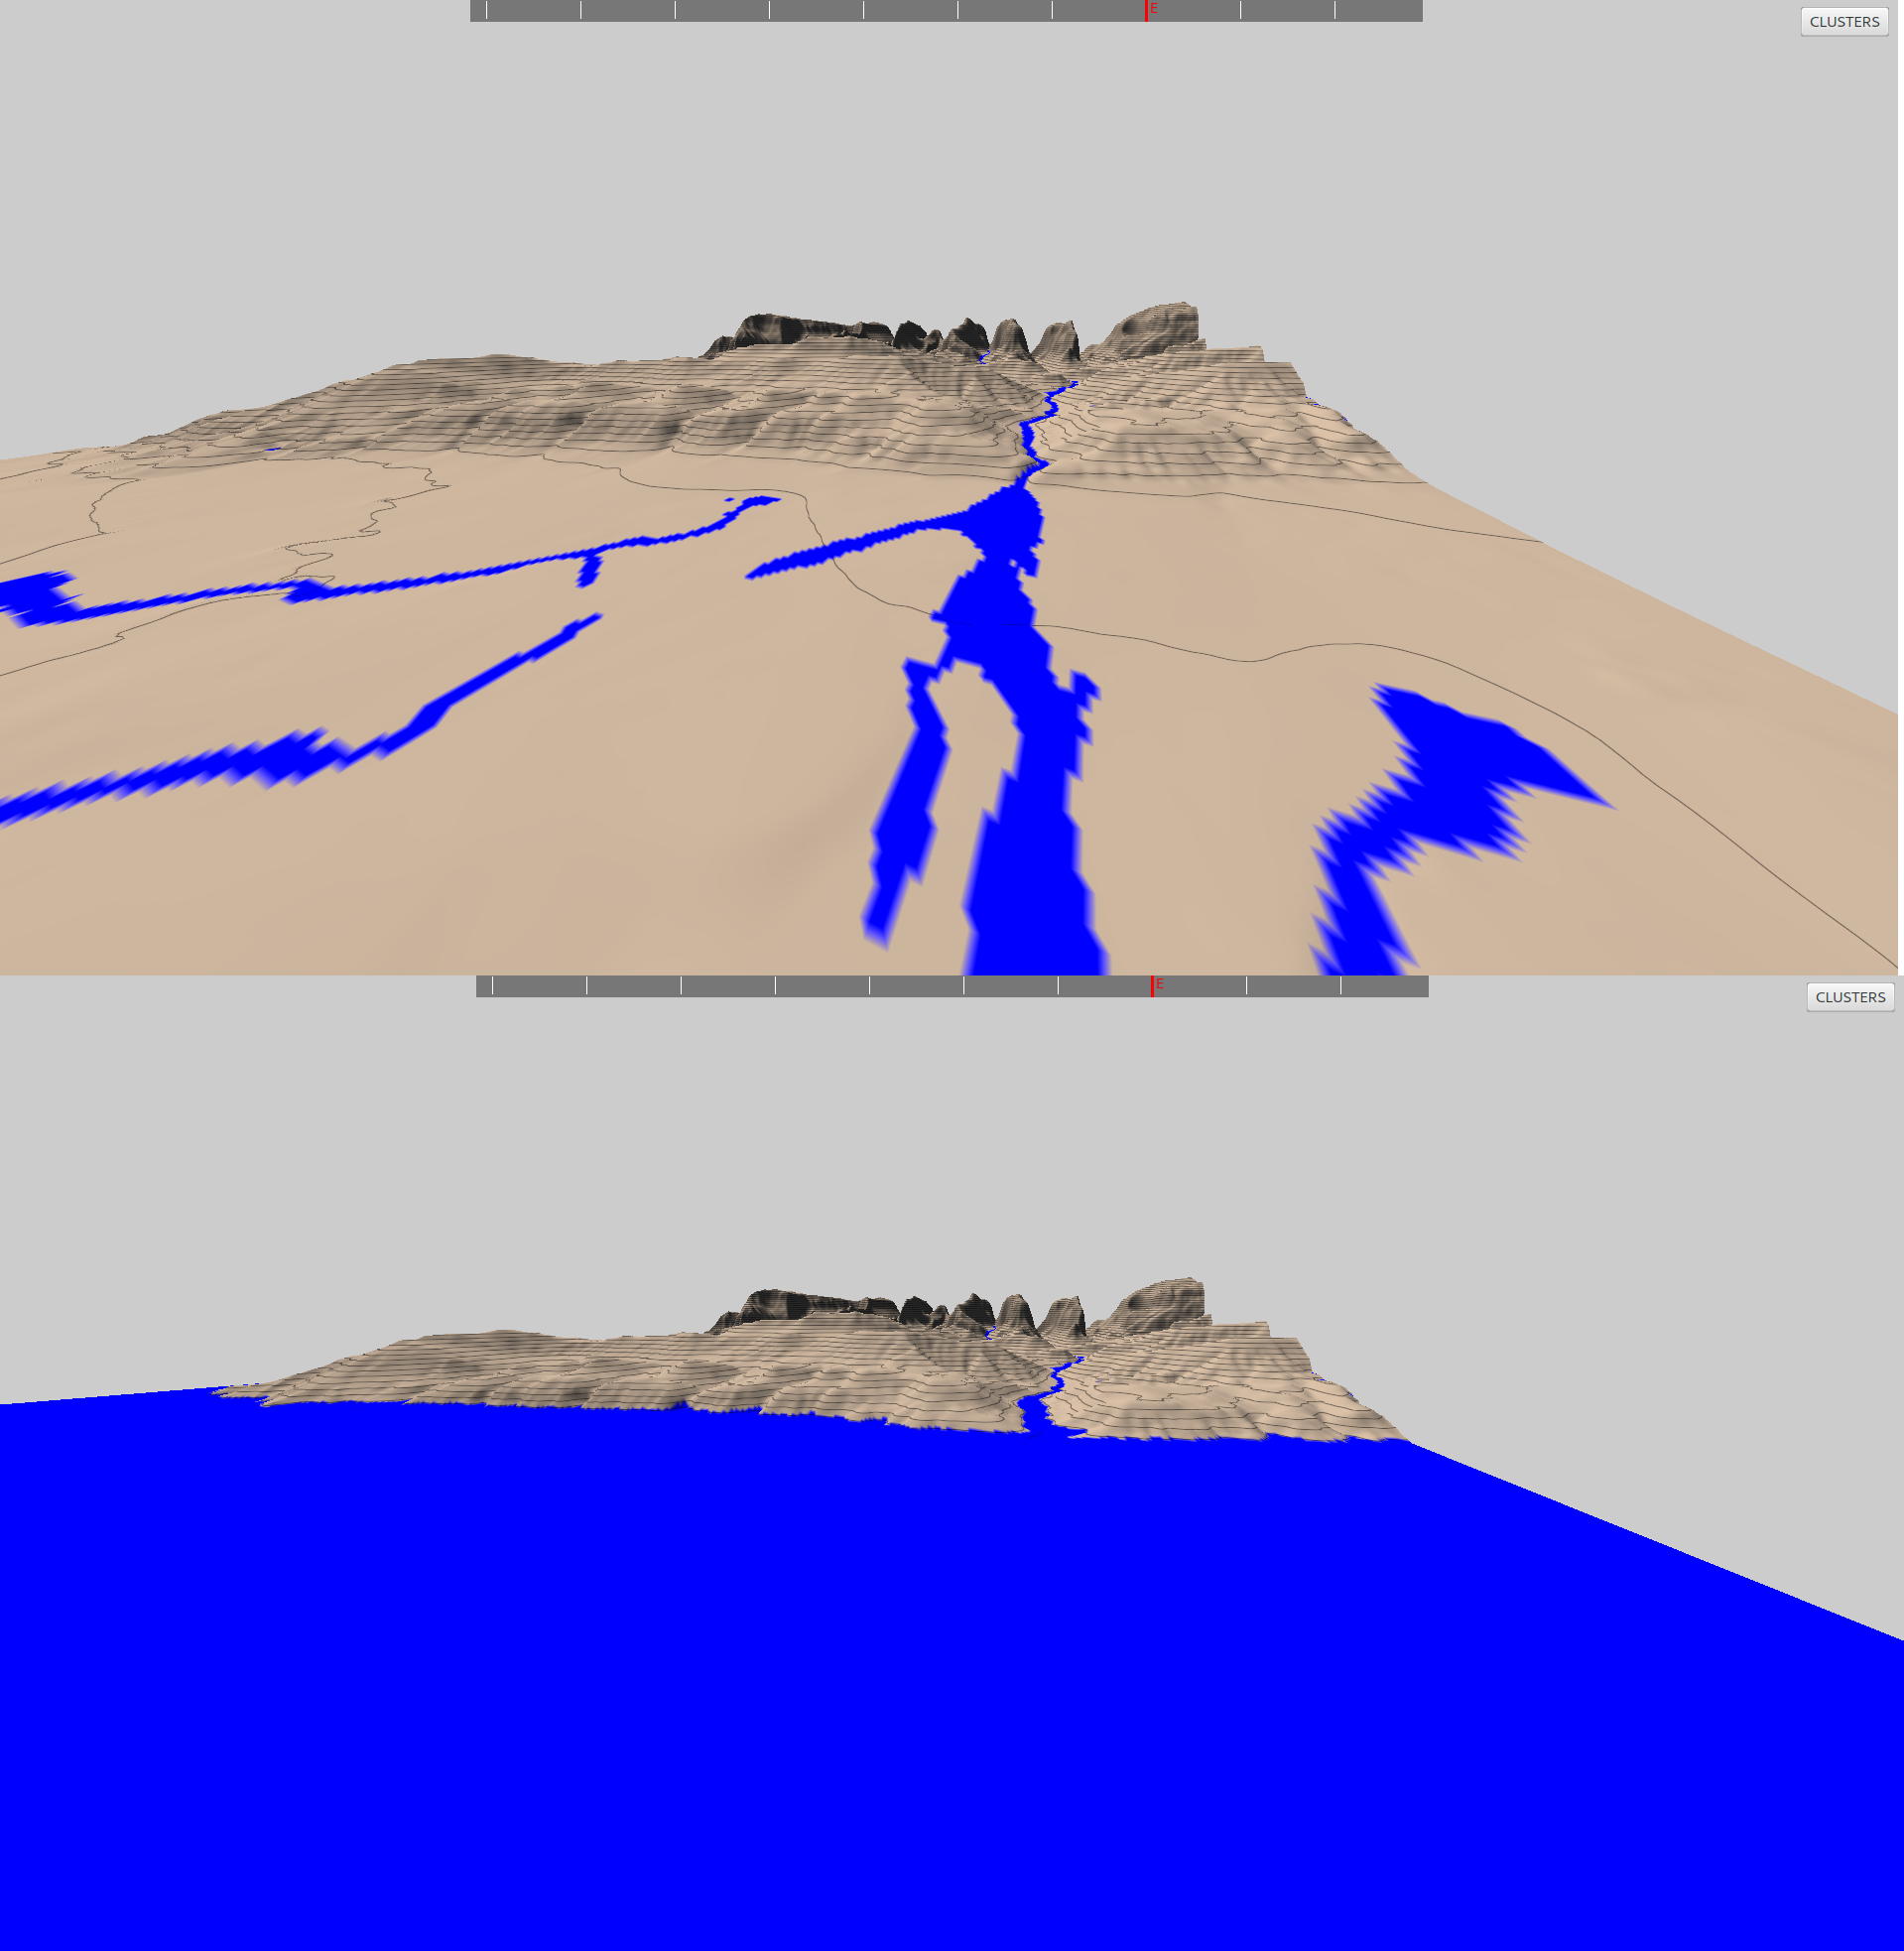
\includegraphics[width=\textwidth]{flood_fill_test_ocean.png}
	\caption{ Terrain before (top) and after (top) using the flood-fill tool to place a large water body (e.g sea or ocean). }	
	\label{fig:flood_fill_test}
\end{figure}


\chapter{Clustering} \label{chap:clustering}

Each point on the terrain has a number of associated resource properties (summarised in table \ref{tab:point_resources}), which are used to determine suitable vegetation and, using an ecosystem simulator, a distribution of this vegetation. However, this simulator is computationally expensive and running it for each terrain vertex is infeasible. As such, to make the number of ecosystem simulations manageable, clustering is performed on the terrain based on the resources associated with individual points. The clustering algorithm used is \textit{K-Means Clustering}, discussed in section \ref{sec:clustering}. To accelerate clustering towards interactive feedback, it is implemented to run on the GPU, details of which can be found in section \ref{sec:gpu_clustering}. To conclude, the performance and results of the clustering algorithm are discussed.

\begin{table}[h]
  \centering
	    \begin{tabular}{|p{6cm}|p{3cm}|p{6cm}|}
		\hline	
  	    \textbf{Resource} & \textbf{Count} & \textbf{Comments} \\
  	    \hline	
  	    Slope & 1 & - \\
		\hline
  	    Temperature & 12 & Temperature for each month \\
		\hline
  	    Illumination & 12 & Illumination for each month \\
		\hline
  	    Soil Humidity & 12 & Soil humidity for each month \\
		\hline
		\end{tabular}
		\caption{Resource properties associated each terrain vertex. Temperature, illumination and soil humidity are monthly values, hence why there are twelve.}
	  \label{tab:point_resources}
\end{table}




\section{K-Means Clustering}

K-means is a well known and broadly used clustering algorithm which is used to group numerical data into clusters based on their euclidean distance from a set of \textit{K} cluster means.\\

Given a set of data points \textit{P} and a configured value \textit{k}, a generic k-means clustering algorithm performs the following:
\begin{enumerate}
\item Choose \textit{K} points at random to act as the seed cluster means \textit{CM}.
\item Iterate through every data point \textit{P$_{n}$} from \textit{P} and calculate its Euclidean distance with each cluster mean of \textit{CM} using equation \ref{eq:cluster_dist_calc}. Point \textit{P} becomes a member of its closest cluster. 
\item Use the members of each cluster to calculate the new cluster means. 
\item Repeat from step 2. 
\end{enumerate}

\begin{equation} \label{eq:cluster_dist_calc}
D(A,B) = \sum_{n=1}^{nvalues} (value_{n}(A) - value_{n}(B)) ^{2}
\end{equation}

Where:
\begin{itemize}
\item \textbf{A} and \textbf{B} are either data points or a cluster mean.
\item \textbf{nvalues} are the number of numerical values associated with each data point.
\item \textbf{value$_{n}$(A)} is the data value \textit{n} of data point A.
\end{itemize}

\subsection{Customising the Euclidean Distance Calculation}

The Euclidean distance calculation outlined in equation \ref{eq:cluster_dist_calc} works well when all values are in the same dimension. Unfortunately, this is not the case for terrain resource data as illumination, slope, temperature and soil humidity are all measured in different units. This means that a one millimetre change in soil humidity will have as musch of an influence on clustering than a one degree change in temperature. To equalise the effect on clustering across all resources, weighting is used when calculating the Euclidean distances (see table \ref{tab:resource_weighting}).

\begin{table}[h]
  \centering
	    \begin{tabular}{|p{6cm}|p{3cm}|}
		\hline	
  	    \textbf{Value} & \textbf{Weighting} \\
  	    \hline	
  	    Slope & 1 \\
		\hline
  	    Temperature & 1 \\
		\hline
  	    Illumination & 1 \\
		\hline
  	    Soil Humidity & 0.1 \\
		\hline
		\end{tabular}
		\caption{Resource weighting when calculating Euclidean distances between.}
	  \label{tab:resource_weighting}
\end{table}

Equation \ref{eq:cluster_dist_calc_real} is used to calculate the Euclidean distance between two terrain positions (or cluster means) \textit{A} and \textit{B} for clustering.

\begin{equation} \label{eq:cluster_dist_calc_real}
D(A,B) = (\textit{S}(A) - \textit{S}(B))^{2} + 
\sum_{n=1}^{12} (\textit{T}_{n}(A) - \textit{T}_{n}(B)) ^{2} + 
(\textit{H}_{n}(A) - \textit{H}_{n}(B)) ^{2} + 
(0.1 \times (\textit{I}_{n}(A) - \textit{I}_{n}(B)) ^{2})
\end{equation}

Where:
\begin{itemize}
\item \textit{S(x)} is the slope of point or cluster mean x.
\item \textit{T$_{n}$(x)} is the temperature of point or cluster mean x at month n.
\item \textit{H$_{n}$(x)} is the soil humidity of point or cluster mean x at month n.
\item \textit{I$_{n}$(x)} is the illumination of point or cluster mean x at month n.
\end{itemize}



\subsection{Choosing Seed Cluster Means}

A downside of classic K-means clustering techniques is that they are non-reproducible. This is because the final clusters depend heavily on the initial seed cluster means. As these are selected at random, different runs will result in different clusters. Reproducibility is important here, however, as if the clusters can't be reproduced neither will the final terrain. \\

A solution to this problem is to initialise the cluster means using pre-determined points on the terrain rather than at random. However, it is also good for the initial seed points to contain distinct resource properties in order for the final clusters to form faster. To attempt to fulfil both these requirements, the seed points are selected at equal distances on the terrain diagonal. This ensures reproducibility as the same seed points will always be selected. This attempts to cater for the second requirement also as it ensures the seed points will have good terrain coverage.

\subsection{Configuring the Number of Clusters \textit{K}}

When vegetation is to be placed on the terrain, \textit{K} ecosystem simulations will need to run. Although larger values of \textit{K} will potentially result in more realistic vegetation distributions, it will also require more processing time. As a consequence, choosing a value for \textit{K} is about finding a balance between realism and processing time. This balance depends on user requirements which is why it is possible to configure it manually. 

\section{GPU Implementation} \label{sec:gpu_clustering}

Performing K-Means clustering is an \textit{O(KN)} problem where K is the number of clusters. As a consequence, given a cluster count, the processing time will increase linearly with terrain area. For large terrains with millions of vertices this could prove time consuming and, consequentially, have a negative effect on user experience. To accelerate the clustering process and maximize user-experience it is implemented to make use of the heavily parallel architecture of the GPU. Below are discussed the details and optimizations of this implementation. \\

\begin{table}[]
  \centering
	    \begin{tabular}{|p{3cm}|p{1.5cm}|p{6cm}|p{5cm}|}
		\hline	
  	    \textbf{Storage Type} &  \textbf{Data Type} & \textbf{Element Count} & \textbf{Usage} \\
		\hline
		3-D Texture & Float & W $\times$ H $\times$ 12 & Monthly Soil Humidity \\
		\hline
		3-D Texture & Float & W $\times$ H $\times$ 12 & Monthly Illumination \\
		\hline
		2-D Texture & Float & W $\times$ H & Temperature \\
		\hline
		2-D Texture & Float & W $\times$ H & Slope \\
		\hline
		3-D Texture & Float & $ \textit{K} \times WorkGroups_{x} \times 13 \times WorkGroups_{y} $ &  Slope and Humidity Reducer \\
		\hline
		3-D Texture & Float & $ \textit{K} \times WorkGroups_{x} \times 2 \times WorkGroups_{y} $ &  Temperature Reducer \\
		\hline
		3-D Texture & Float & $ \textit{K} \times WorkGroups_{x} \times 12 \times WorkGroups_{y} $ & Daily Illumination Reducer \\
		\hline
		\end{tabular}
		\caption{Global memory allocations necessary for the GPU implementation of K-Means clustering. \textit{W} and \textit{H} are the width and height of the terrain respectively. \textit{WorkGroups$_{x}$} and \textit{WorkGroups$_{y}$} are the horizontal and vertical workgroup count respectively.}
	  \label{tab:clustering_mem_allocs}
\end{table}

\subsection{Calculating cluster membership}

Given the cluster means for iteration \textit{i}, the algorithm must determine to which cluster each terrain vertex belongs. To do so efficiently, each GPU core is associated a unique vertex and is responsible for determining it's cluster membership.

\subsection{Calculating the new cluster means}

Once all terrain vertices have been assigned to a cluster, they must be iterated over in order to calculate the new means of each cluster.\\

Within a work-group (group of cores which are guaranteed to run in parallel and have access to shared memory), when each core calculates it's distance from individual cluster means, it loads its associated resource data into a unique index of fast-access shared memory. It also stores in shared memory the calculated cluster membership. This data is then used to calculate, within each work-group, \textit{k} new work-group cluster means, in parallel. The \textit{k} work-group cluster means are then stored to global memory along with the member count for each cluster.\\

Finally, the global cluster means are calculated by \textit{k} cores in parallel using the means calculated for each individual work group along with their associated member counts.\\

\subsection{Storage Optimization}

The temperature on the terrain increases linearly with altitude. As such, even though the temperature changes monthly on the terrain, the temperature difference between two points \textit{P$_{a}$} and \textit{P$_{b}$} will remain constant throughout the year. Calculating the Euclidean distance from a given point \textit{A} to a cluster mean is identical to calculating the difference between two points on the terrain. As a consequence, it is only necessary to use a single months temperature data to establish terrain clusters, saving vital GPU storage space.

\subsection{Minimizing CPU to GPU data transfers}

As mentioned previously, copying data to and from CPU to GPU is a costly process. To prevent these costly transfer operations, all data required for the clustering algorithm (table \ref{tab:clustering_mem_allocs}) is copied to the GPU at the start of the clustering process and no further transfers are performed until completion. \\
\section{Performance}

As mentioned previously, the user must specify the requested cluster count \textit{k}. In order to find a suitable value for \textit{k}, the user will need to trial a number of different values. To minimize any negative effect on user-experience, therefore, it is important the clustering performs in near real-time, irrespective of terrain size and cluster count.\\

The performance of the CPU and GPU clustering implementations are analysed below along with an evaluation of the GPU speed-up. In order to evaluate the performance of the different implementations, the clustering time is analysed in relation to terrain size and cluster count. In order to accurately compare their performance, the same terrains are used with identical resources specified. 

\subsection{CPU Performance}

Figure \ref{fig:cpu_clustering_performance} shows the time it takes for the clustering to run with different terrain sizes and number of clusters. Notable results from this data are:
\begin{itemize}
\item Ten clusters take on average five times longer to generate than a single cluster.
\item The same number of clusters take on average four times longer to generate for a terrain of size 512 by 512 than for terrain of size 256 by 256. This increases to six when comparing a terrain of size 512 by 512 with one of size 1024 by 1024.
\end{itemize}

\begin{figure}
\center
	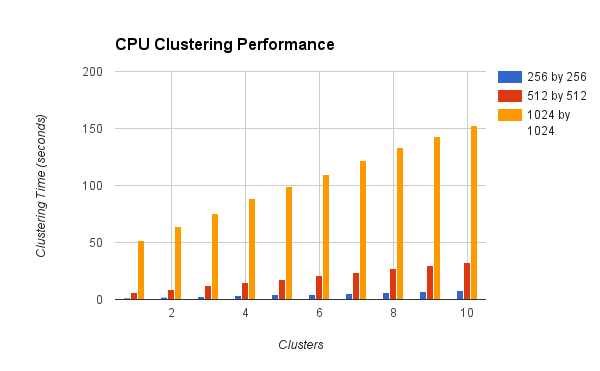
\includegraphics[width=\textwidth]{clustering_cpu_performance.png}
	\caption{ Time it takes for the clustering process to complete on the CPU depending on the cluster count. The analysis was performed for terrains of size: 256 by 256 (blue), 512 by 512 (red) and 1024 by 1024 (orange).}	
	\label{fig:cpu_clustering_performance}
\end{figure}

Although the clustering time is reasonable for smaller terrains, this processing time increases sharply with the terrain size. This is especially true when combined with an increase in the number of clusters to generate. 

\subsection{GPU Performance}

The same tests run using the GPU implementation are displayed in figure \ref{fig:gpu_clustering_performance}. Notable results are:

\begin{itemize}
\item Ten clusters take on average twice the time of a single cluster to generate.
\item The processing time increases proportionally with the number of terrain vertices.
\end{itemize}

\begin{figure}
\center
	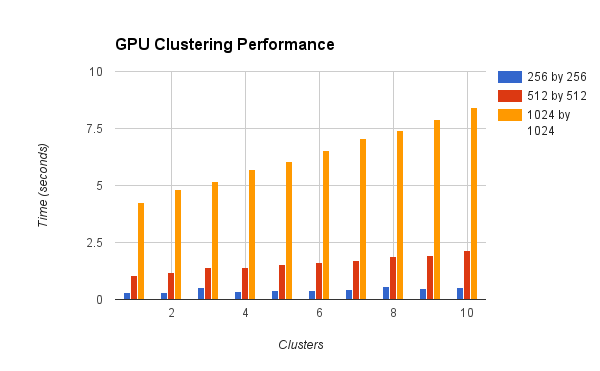
\includegraphics[width=\textwidth]{clustering_gpu_performance.png}
	\caption{ Time it takes for the clustering process to complete on the GPU depending on the cluster count. The analysis was performed for terrains of size: 256 by 256 (blue), 512 by 512 (red) and 1024 by 1024 (orange).}	
	\label{fig:gpu_clustering_performance}
\end{figure}

Because different clusters are managed in parallel on the GPU, increasing the cluster count has a much smaller impact on performance than for the CPU implementation.\\

Individual terrain vertices are managed in parallel on the GPU. Although this greatly speeds up the clustering process, because the number of terrain vertices far outnumber the number of GPU cores, the clustering time is still heavily impacted by increases in terrain size.


\subsection{GPU Speed-up}

Figures \ref{fig:clustering_cpu_v_gpu_256}, \ref{fig:clustering_cpu_v_gpu_512} and \ref{fig:clustering_cpu_v_gpu_1024} compare the CPU and GPU clustering processing time for square terrains of size 256, 512 and 1024 respectively. These graphics show that the GPU greatly outperforms the CPU, irrespective of terrain size and cluster count. Also visible in these graphics is the increased sensitivity to the cluster count of the CPU implementation where the clustering time increases much more rapidly. \\

\begin{figure}
\center
	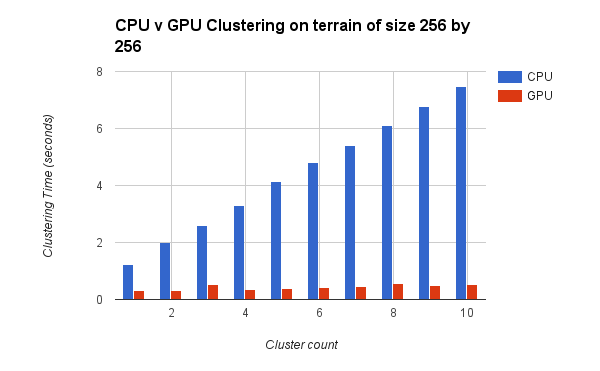
\includegraphics[width=\textwidth]{clustering_cpu_v_gpu_256.png}
	\caption{ Comparison of CPU (blue) and GPU (red) clustering times on a 256 by 256 terrain.}	
	\label{fig:clustering_cpu_v_gpu_256}
\end{figure}

\begin{figure}
\center
	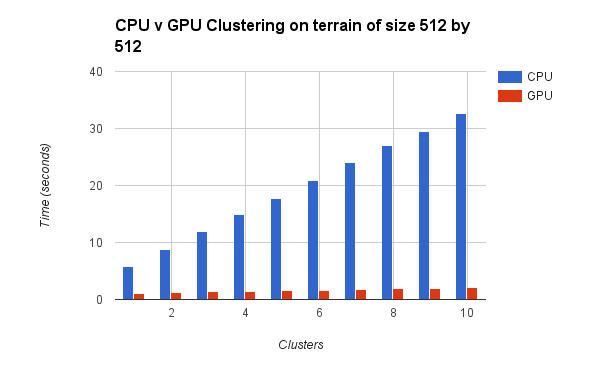
\includegraphics[width=\textwidth]{clustering_cpu_v_gpu_512.png}
	\caption{ Comparison of CPU (blue) and GPU (red) clustering times on a 512 by 512 terrain.}	
	\label{fig:clustering_cpu_v_gpu_512}
\end{figure}

\begin{figure}
\center
	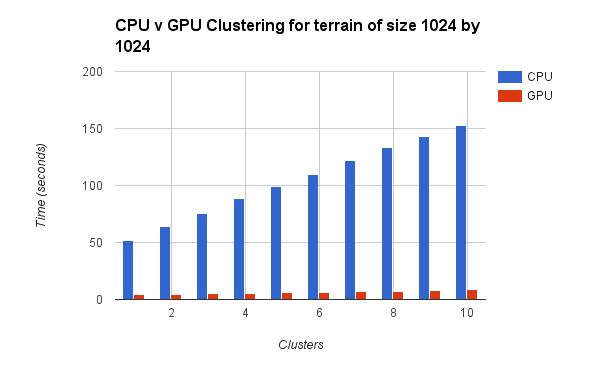
\includegraphics[width=\textwidth]{clustering_cpu_v_gpu_1024.png}
	\caption{ Comparison of CPU (blue) and GPU (red) clustering times on a 1024 by 1024 terrain.}	
	\label{fig:clustering_cpu_v_gpu_1024}
\end{figure}

As well as confirming the increased sensitivity to cluster count of the CPU implementation, figure \ref{fig:clustering_cpu_v_gpu_speedup} which plots the GPU speed-up for each terrain size and cluster count, shows that this speed-up also increases with terrain size. 

\begin{figure}
\center
	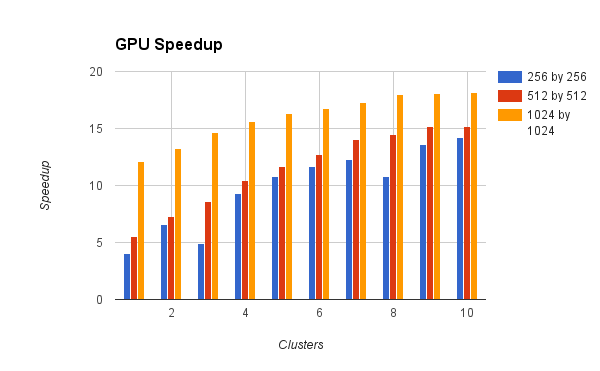
\includegraphics[width=\textwidth]{clustering_cpu_v_gpu_speedup.png}
	\caption{ Calculated clustering speed-up of the GPU implementation compared to the CPU implementation for square terrains of size 256 (blue), 512 (red) and 1024 (yellow).}	
	\label{fig:clustering_cpu_v_gpu_speedup}
\end{figure}
\section{Overlay and Cluster Descriptions}

When clustering is complete, each point on the terrain is associated with one of \textit{k} unique clusters. To make this association apparent to the user a cluster overlay is displayed. The clustering overlay attributes a unique color to each cluster and subsequently to each terrain vertex based on cluster membership (see figure \ref{fig:cluster_overlay}). Along with the terrain overlay, a dialogue shows the properties (color, member count, resources) of each cluster (see appendix \ref{AppendixA}).

\begin{figure}
\center
	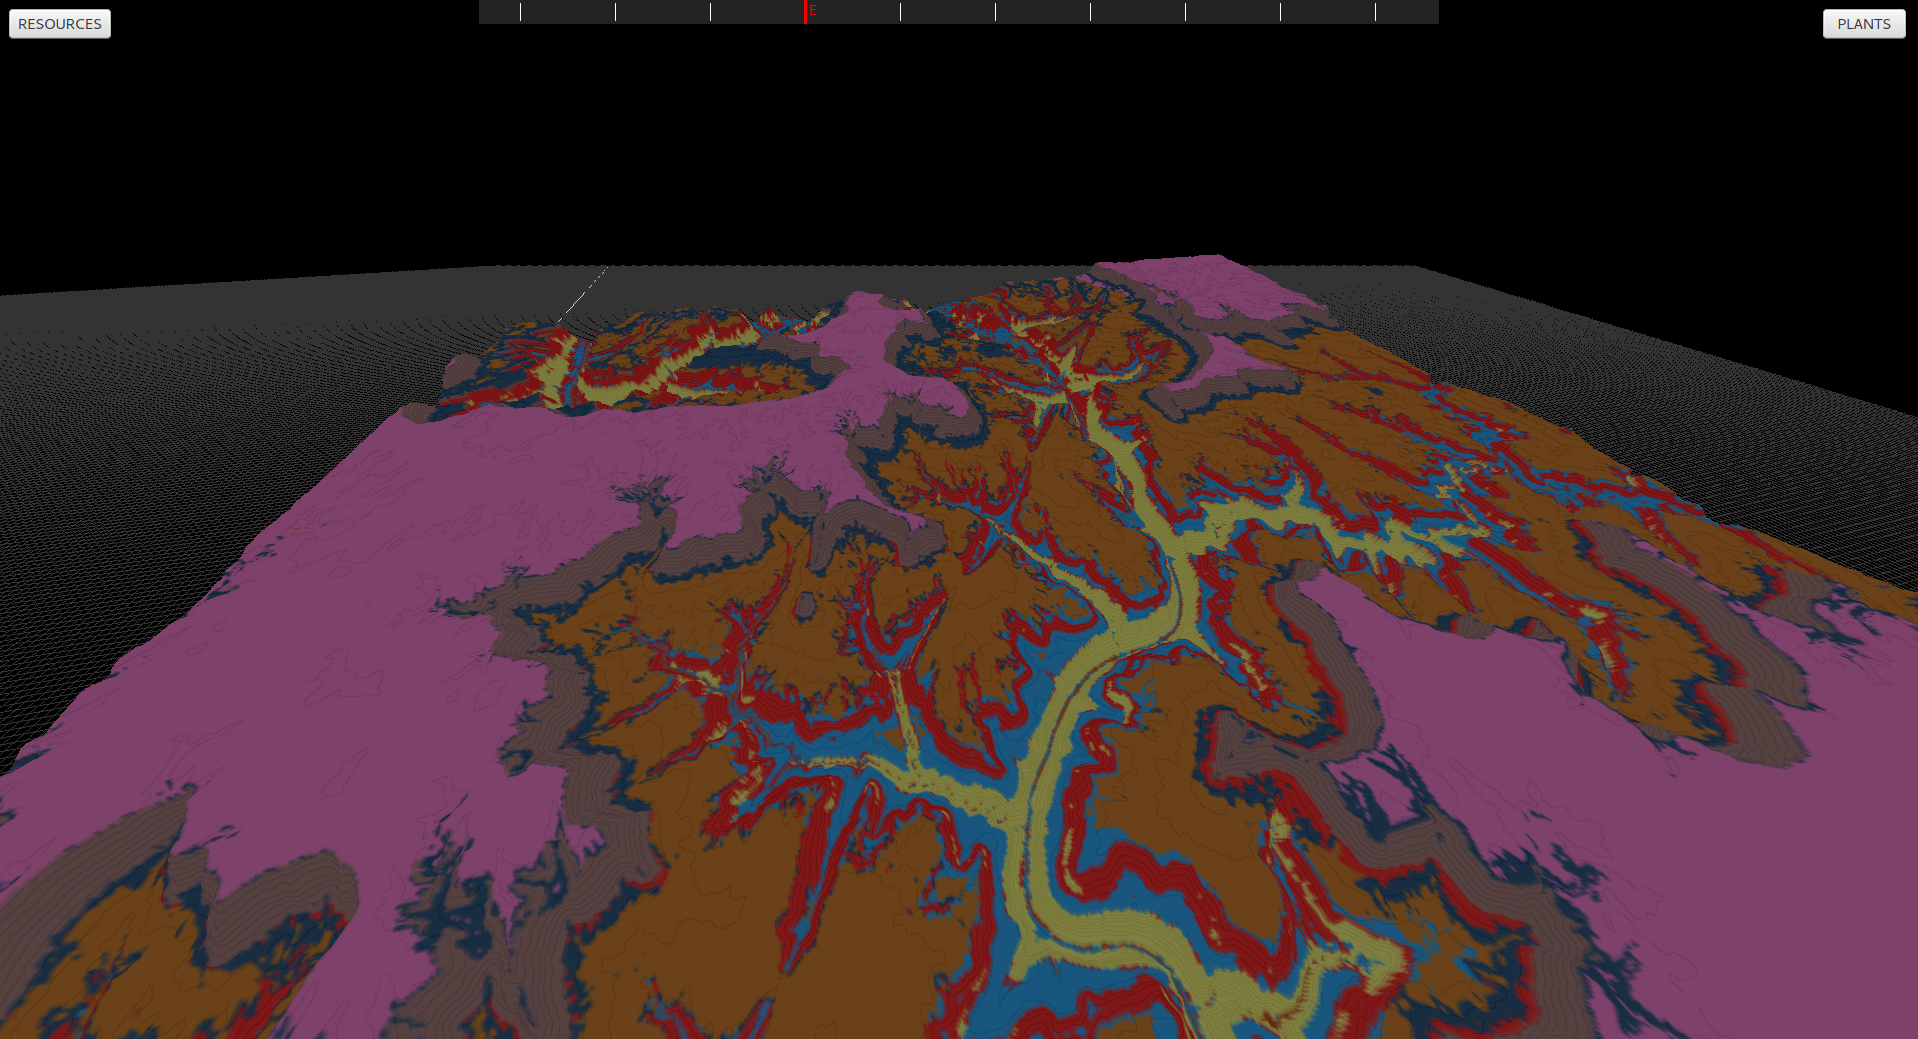
\includegraphics[width=\textwidth]{cluster_overlay.png}
	\caption{ \textit{Colour coded cluster overlay. Using this it is possible to easily identify the clusters associated to each terrain vertex.}}	
	\label{fig:cluster_overlay}
\end{figure}

\section{Results}

To test the clustering algorithm, a terrain is loaded, it's resources edited and five clusters produced. These clusters are subsequently analysed to ensure they successfully detect distinct resource features on which to cluster.\\

The terrain used is a model of the Grand Canyon using data from the US Geological Survey \protect\footnotemark \footnotetext{\url{http://www.usgs.gov}}. This terrain is chosen as its canyons and crevasses make ground illumination vary greatly.\\

The following resource edits were performed on the terrain:

\begin{itemize}
\item \textit{Latitude}: Set to zero degrees (equator)
\item \textit{Soil Infiltration}: 5 millimetres for all terrain points with a slope under 30 degrees. All points with a slope over 30 degrees were set to 0 to simulate a cliff.
\item \textit{Rainfall}: See table \ref{tab:clustering_test_rainfall}.
\item \textit{Temperature}: 0 degrees at 0 meters in December. 15 degrees at 0 metres in June. Lapse rate at default value of 6.4 degrees per thousand metres.
\end{itemize}

The resulting terrain clusters that form are displayed in figure \ref{fig:clustering_test_resulting_clusters} and summarized in appendix \ref{AppendixA}.

\begin{table}[]
  \centering
	    \begin{tabular}{|p{5cm}|p{5cm}|}
	    \hline
	    \textbf{Month} & \textbf{Rainfall (mm)}\\
		\hline
	    Jan & 13 \\
	    \hline
	    Feb & 15 \\
	    \hline
	    Mar & 14 \\
	    \hline
	    Apr & 9 \\
	    \hline
	    May & 6 \\
	    \hline
	    Jun & 18 \\
	    \hline
	    Jul & 18 \\
	    \hline
	    Aug & 22 \\
	    \hline
	    Sep & 15 \\
	    \hline
	    Oct & 11 \\
	    \hline
	    Nov & 9 \\
	    \hline
	    Dec & 16 \\
	    \hline
		\end{tabular}
		\caption{Monthly rainfall configured for the clustering tests.}
	  \label{tab:clustering_test_rainfall}
\end{table}

\begin{figure}
\center
	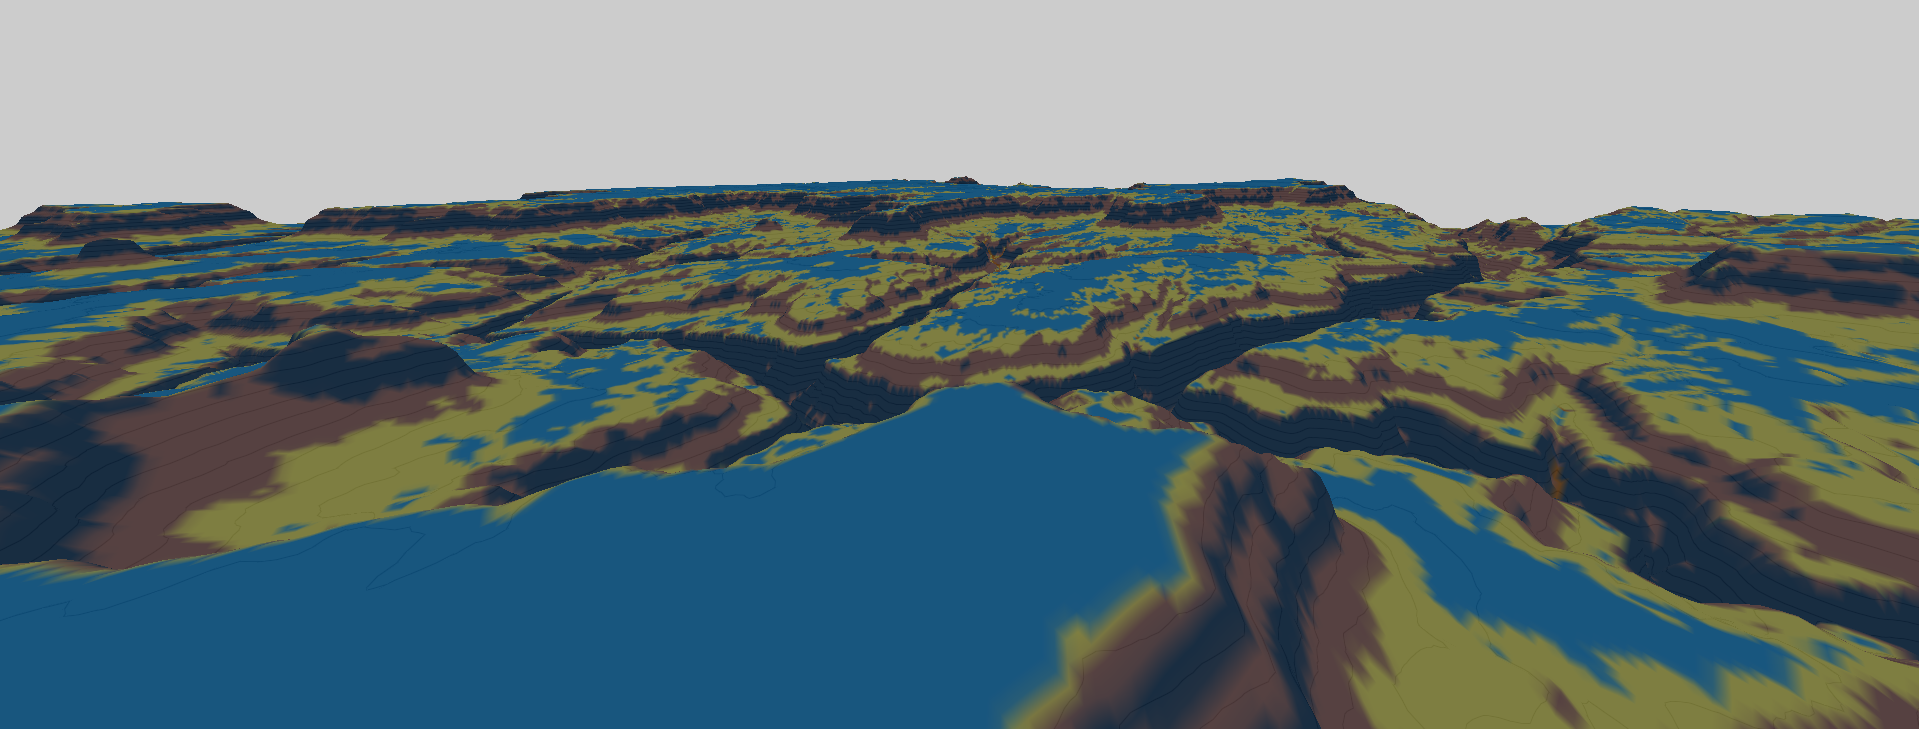
\includegraphics[width=\textwidth]{clustering_test_resulting_clusters.png}
	\caption{ \textit{Clustering test: Resulting terrain clusters}}	
	\label{fig:clustering_test_resulting_clusters}
\end{figure}

\begin{figure}
\center
	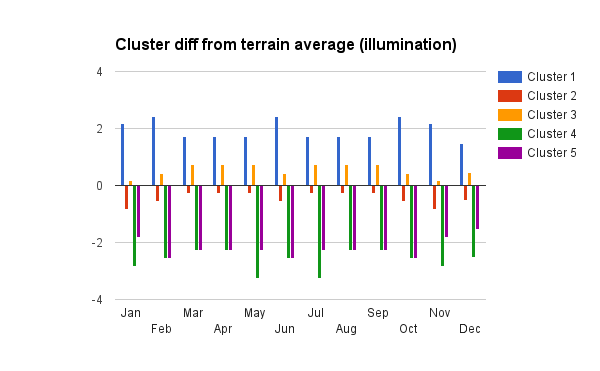
\includegraphics[width=\textwidth]{clustering_graph_illumination_diff.png}
	\caption{ \textit{Monthly illumination for each cluster and the average over the whole terrain.}}	
	\label{fig:clustering_graph_illumination}
\end{figure}

\begin{figure}
\center
	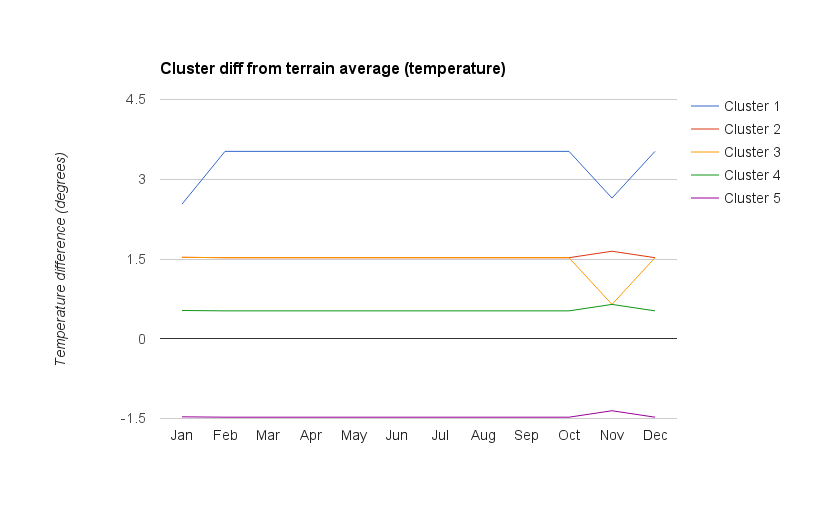
\includegraphics[width=\textwidth]{clustering_graph_temp_diff.png}
	\caption{ \textit{Monthly temperature for each cluster and the average over the whole terrain. Cluster 2 has the same values as cluster 4.}}	
	\label{fig:clustering_graph_temp}
\end{figure}

\begin{figure}
\center
	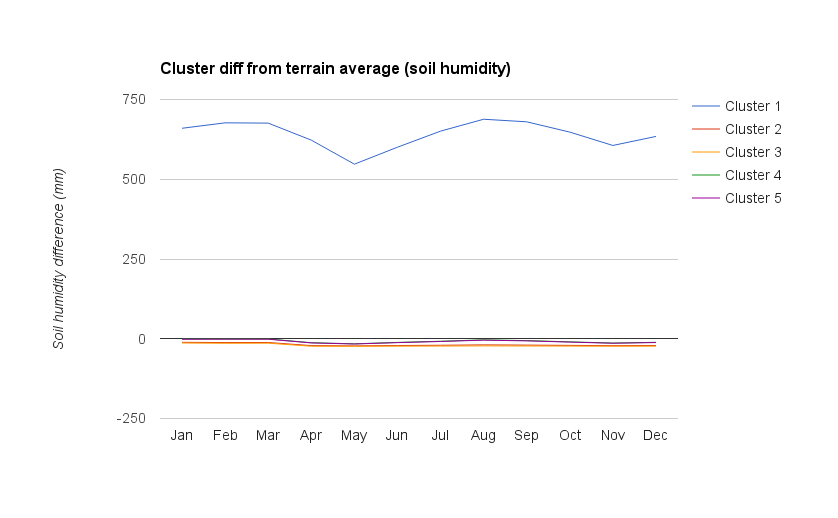
\includegraphics[width=\textwidth]{clustering_graph_soil_humidity_diff.png}
	\caption{ \textit{Soil humidity for each cluster (same for every month) and the average over the whole terrain.}}	
	\label{fig:clustering_graph_humidity}
\end{figure}

\begin{table}[]
  \centering
	\begin{tabular}{|p{5cm}|p{5cm}|}
	\hline
	\textbf{Cluster ID} & \textbf{Slope difference (degrees)}\\
	\hline
	1 & -2.5 \\	
	\hline
	2 & 36.7\\	
	\hline
	3 & 59.5\\	
	\hline
	4 & -18\\	
	\hline
	5 & -53.5\\		
	\hline
	\end{tabular}
	\caption{ Difference of slope between the means of each cluster and the terrain mean.}
	\label{tab:clustering_slope_mean}
\end{table}

Figures \ref{fig:clustering_graph_illumination}, \ref{fig:clustering_graph_temp}, \ref{fig:clustering_graph_humidity} and table \ref{tab:clustering_slope_mean} show how much each cluster's illumination, temperature, soil humidity and slope vary from the terrain's average.\\ 

From figure \ref{tab:clustering_test_cluster_variance}, which summarises the resource variance of each cluster, it is possible to identify key terrain features the represent, notably: \textit{Cluster 1} is formed of the data points within the flat bottom of the canyon where the rivers form. Hence the low temperature caused by the low altitude, the low illumination caused by the surrounding canyon walls casting shade, the extremely high humidity caused by the river stream passing through and the flat bottom causing the slope to be very low. \textit{Cluster 2} constitutes the points at the top of the canyon cliffs where slope reduces. Hence the high slope and the low humidity (water run-off). \textit{Cluster 3} contains the data points on the cliffs of the terrain, hence the high slopes, low humidity (water run-off) and low illumination (cliffs often in the shade). \textit{Cluster 4} is formed of the data points most similar to the terrain mean, hence its limited variance. \textit{Cluster 5} is formed of the areas of high altitudes where the surface is flat, illumination is high (nothing to shade it) and temperatures are low.\\

\begin{table}[]
  \centering
	    \begin{tabular}{|p{3cm}|p{3cm}|p{3cm}|p{3cm}|p{3cm}|}
		\hline	
  	    \textbf{Cluster} &  \textbf{Illumination} & \textbf{Temperature} & \textbf{Soil Humidity} & \textbf{Slope} \\
		\hline
		\textbf{1} & 4(-) & 5(+)$^{*}$ & 5(+)$^{*}$ & 1(-) \\
		\hline
		\textbf{2} & 2(-) & 4(+) & 3(-) & 3(+) \\
		\hline
		\textbf{3} & 5(-)$^{*}$ & 2(+) & 4(-)$^{*}$ & 5(+)$^{*}$ \\
		\hline
		\textbf{4} & 1(+) & 1(+) & 1(-) & 2(-) \\
		\hline
		\textbf{5} & 3(+)$^{*}$ & 3(-)$^{*}$ & 2(-) & 4(-)$^{*}$ \\
		\hline
		\end{tabular}
		\caption{Comparison of cluster feature variance from terrain average on a ranking of 1 (least) to 5 (most). The symbol states whether the variance is positive (+) or negative (-). The minimums and maximums for each resource are represented with a $^{*}$. }
	  \label{tab:clustering_test_cluster_variance}
\end{table}

\chapter{Vegetation}

Vegetation is an essential part of rural terrains is vegetation. Available resources determine which plant species are able to grow and to what extent they strive in a given environment. Reproducing this link between species and climate is essential to determining suitable vegetation and, subsequently, generating plausible terrains. \\

To determine environments suited for given species, they are configured with associated resource requirements as outlined in section \ref{sec:plant_species}. Given these properties, it is possible to automatically filter out ill-suited plants. Information about this automatic filtering is outlined in section \ref{sec:plant_suitability_filtering}.\\

Although a multitude of plants can grow in a given environment, some will naturally flourish more than others. This can be because resources are more suitable or they have a faster, more aggressive growth rate. To model this intra-species battle for resources and  determine a suitable vegetative state, an ecosystem simulator is used, details of which can be found in section \ref{sec:ecosystem_simulator}.\\

The ecosystem simulator is computationally expensive and can take some time to determine a valid distribution. The simulation time is dependent on the number of plant instances, the simulation area and the timespan. To accelerate the process, the ecosystem simulator is run over a small area and the resulting distribution analysed in order to efficiently reproduce it on larger areas. A caching system is also used to prevent users from having to run the same costly simulation more than once. Information about these features is discussed in section \ref{sec:dist_analysis_and_rep}.

\section{Plant Species} \label{sec:plant_species}

A database is used to store all plant species and their associated properties, which are used to determine their ability to grow in a given environment and, subsequently, deduce a plausible distribution using the ecosystem simulator. A dedicated tool can be used to interact directly with the database in order to add, remove and edit this data.\\
When configuring a new species it is necessary to specify a set of associated properties. These properties can be split into two main categories: \textit{simulation-based} and \textit{environment-based}. \textit{Simulation-based} properties are those used only by the ecosystem simulator to simulate the growth and spawning of new plants. \textit{Environment-based} properties are those used by the simulator to calculate the strength of the plant but also to determine whether or not it is suited to given environments. Each are discussed below and summarized in table \ref{tab:specie_properties}.\\

\begin{table}[]
  \centering
	    \begin{tabular}{|p{4cm}|p{7cm}|p{2cm}|}
		\hline	
		\textbf{Property} & \textbf{Value} & \textbf{Units} \\
		\hline
		\multirow{2}{*}{\textbf{Slope}} & \multicolumn{1}{l|}{Start of decline} & \multicolumn{1}{l|}{Degrees} \\\cline{2-3}
        						   & \multicolumn{1}{l|}{Maximum} & \multicolumn{1}{l|}{Degrees} \\
		\hline
		\multirow{3}{*}{\textbf{Growth}} & \multicolumn{1}{l|}{Maximum canopy} & \multicolumn{1}{l|}{Centimetres} \\\cline{2-3}
        						   & \multicolumn{1}{l|}{Maximum root size} & \multicolumn{1}{l|}{Centimetres} \\\cline{2-3}
                               & \multicolumn{1}{l|}{Maximum height} & \multicolumn{1}{l|}{Centimetres} \\
		\hline
		\multirow{2}{*}{\textbf{Ageing}} & \multicolumn{1}{l|}{Start of decline} & \multicolumn{1}{l|}{Months} \\\cline{2-3}
        						   & \multicolumn{1}{l|}{Maximum age} & \multicolumn{1}{l|}{Months} \\
		\hline    
		\multirow{2}{*}{\textbf{Seeding}} & \multicolumn{1}{l|}{Maximum seeding distance} & \multicolumn{1}{l|}{Metres} \\\cline{2-3}
        						   & \multicolumn{1}{l|}{Annual seed count} & \multicolumn{1}{l|}{ - } \\
		\hline    
		\multirow{4}{*}{\textbf{Illumination}}
								& \multicolumn{1}{l|}{Start of prime} & \multicolumn{1}{l|}{hours} \\\cline{2-3}
								& \multicolumn{1}{l|}{End of prime} & \multicolumn{1}{l|}{hours} \\\cline{2-3}
								& \multicolumn{1}{l|}{Minimum} & \multicolumn{1}{l|}{hours} \\\cline{2-3}
								& \multicolumn{1}{l|}{Maximum} & \multicolumn{1}{l|}{hours} \\
		\hline   
		\multirow{4}{*}{\textbf{Humidity}}
								& \multicolumn{1}{l|}{Start of prime} & \multicolumn{1}{l|}{millimetres} \\\cline{2-3}
								& \multicolumn{1}{l|}{End of prime} & \multicolumn{1}{l|}{millimetres} \\\cline{2-3}
								& \multicolumn{1}{l|}{Minimum} & \multicolumn{1}{l|}{millimetres} \\\cline{2-3}
								& \multicolumn{1}{l|}{Maximum} & \multicolumn{1}{l|}{millimetres} \\
		\hline    
		\multirow{4}{*}{\textbf{Temperature}}
								& \multicolumn{1}{l|}{Start of prime} & \multicolumn{1}{l|}{degrees} \\\cline{2-3}
								& \multicolumn{1}{l|}{End of prime} & \multicolumn{1}{l|}{degrees} \\\cline{2-3}
								& \multicolumn{1}{l|}{Minimum} & \multicolumn{1}{l|}{degrees} \\\cline{2-3}
								& \multicolumn{1}{l|}{Maximum} & \multicolumn{1}{l|}{degrees} \\
		\hline                                                                           
		\end{tabular}
	\label{tab:specie_properties}	
	\caption{\textit{Summary of the properties which must be configured with each plant species.}}
\end{table}

\subsection{Simulation-based Species Properties}

%Growth
To model the growth of a plant species in the ecosystem simulator, it is necessary to specify: \textit{Maximum height}, \textit{maximum canopy width} and \textit{maximum root size}. Using these along with the specie's ageing properties, it is possible to simulate the plants vertical growth (height), horizontal growth (canopy) and root coverage. A plants height and canopy width is also used to determine the shade it projects on other plants during the simulation. Furthermore, the plant's root growth is used to determine how far the plant can reach to fetch soil water. Note that a maximum canopy width of zero can be specified to model plants with no canopy.\\

%Ageing
Biological life-cycle varies greatly between plant species. Whereas annual and biennials have a fixed lifespan of one and two years, respectively, perennial plant species can live far longer. To model the life-cycle of different plant species they must be configured with an associated \textit{age of start of decline} and \textit{maximum age}. Using these two values, it is possible to simulate a plant getting weaker and, therefore, becoming more susceptible to domination from surrounding plants.\\

%Seeding
It is necessary to replicate the spawning of offspring in the ecosystem simulator for two core reasons: \textit{Propagation}: Plants propagate on a terrain by producing new offspring which attempt to spawn and invade different areas. \textit{Succession}: New plants spawn to later succeed older and weaker plants of the same specie.\\ 
The two most common ways for plants to spawn new offspring is through sexual and asexual reproduction. Asexual reproducing species often spawn cloned offspring through budding (e.g potato). Sexual reproducing species, on the other hand, require chromosome exchange between males and females in order to produce unique offspring often propagated via seeds or spores. Although biologically different, both can be considered identical for the sole purpose of modelling propagation and succession. The reproduction characteristics of a given species which will influence \textit{propagation} and \textit{succession} in the simulation and therefore need to be configured, are the \textit{number of offspring produced annually} and the \textit{maximum distance from source to offspring}.\\

\subsection{Environment-based Species Properties}

%SLOPE
Steep slopes causes essential water and soil nutrients to run-off, making them less rich and, therefore, less suited to plant growth \cite{Kapolka2001}. The slope angle can also cause larger species to struggle in supporting their own biomass. For this reason, steeper slopes often cater better to smaller plant species (grass, shrub, etc.). To model the effect of slope on given plant species, when configuring a new plant species, the \textit{slope of start of decline} and \textit{maximum slope} must be configured.\\

%Illumination
Illumination, soil humidity and temperature also have a great impact on plant growth and survival \cite{Fourcaud2008}.\\
Whereas some species thrive in shaded undergrowth, others require direct illumination all year round. Soil water deposited into the soil by either rainfall or existing groundwater is absorbed by plant roots and is vital to their development and survival. Some species have evolved to survive in arid climates with very little water, others require frequent downpours of rain. To simplify water requirement specifications for different plant species, we ignore groundwater and consider rainfall as the plants only source of water. Some species are able to withstand extremely low temperatures (e.g at high altitudes), others have the ability to survive in extremely hot temperatures (e.g deserts).\\
To configure the illumination, soil humidity and temperature requirements of a given species, it is necessary to configure for each the \textit{minimum}, \textit{prime range} and \textit{maximum}. The minimum represents the minimum illumination (hours), soil humidity (millimetres) or temperature (degrees) necessary for the species survival, the prime range are the values at which the resource is deemed optimal and the maximum is the upper limit after which the plant is unable to survive.


\section{Plant Suitability Filtering} \label{sec:plant_suitability_filtering}

Once the terrain clusters have been generated, the user must specify the plant species to incorporate. The ecosystem simulator is then used to determine a suitable distribution for the species given the resources associated with the individual clusters.\\

Rather than permit the user to select any plant from the database, including those unable to grow, a filtering pass is performed in order to display only the plants best able to survive. This is useful as it prevents users from triggering an ecosystem simulation run with species that are guaranteed not to survive. To determine whether a given species is suited, a \textit{species suitability score} is calculated for each species based on the resources of each cluster. \\

As well as being used to filter out ill-suited species, this suitability score also highlights the species best suited to the given environment and could, as a consequence, prove to be useful information for the user when selecting plant species. Various methods are used to effectively communicate the suitability score, details of which are discussed below.

\subsection{Calculating the Specie Suitability Score}

The species suitability score associated with a given species, \textit{S}, for cluster \textit{C}, illustrates how suited species \textit{S} is to the environment of cluster \textit{C} on a range from 0 (completely ill-suited) to 100 (perfect conditions). To calculate this, the resource requirements of species \textit{S} are matched with the resource availability of cluster \textit{C}. To determine this score, it is first necessary to determine the specie's suitability to the environment in terms of \textit{slope}, \textit{illumination}, \textit{soil humidity} and \textit{temperature}. A separate score is calculated for each as discussed below. Note that no filtering is based on illumination as it varies during the simulation as the canopy of taller plants shade that of the smaller ones.\\

The slope suitability score determines how well suited the species is in terms of slope and is calculated as illustrated in equation \ref{eq:slope_suitability_score}.\\

\begin{equation}
\centering
SS(S,x) = 
\begin{cases}
    100, & \text{if } x \leq S_{sod} \\
    0, & \text{if } x \geq S_{max} \\
	(1-\frac{x-S_{sod}}{S_{max}-S_{sod}}) \times 100, & \text{otherwise}
\end{cases}
\label{eq:slope_suitability_score}
\end{equation}
Where: \textit{SS(S,x)} is the slope suitability score for specie \textit{S} given slope \textit{x}; \textit{S$_{sod}$} is slope of start of decline configured for specie \textit{S}; \textit{S$_{max}$} is the maximum slope configured for specie \textit{S}.

Because the soil humidity and temperature vary on a monthly basis, it is necessary to calculate the score for each month as illustrated in equation \ref{eq:monthly_score}. The mean of these twelve months is then calculated as illustrated in equation \ref{eq:avg_score} to represent the overall suitability score for the given resource.

\begin{equation}
\centering
MRS(S,r,x) = 
\begin{cases}
    0, & \text{if } x < S_{min}(r) \text{ or } x > S_{max}(r) \\
    \frac{x - S_{min}(r)}{S_{ps}(r) - S_{min}(r)} \times 100, & \text{if } x \in [S_{min}(R),S_{ps}(R)] \\
    100, & \text{if } x \in [S_{prime_start}(r),S_{prime_end}(r)] \\
    (1 - \frac{x - S_{pe}(r)}{S_{max}(r)-S_{pe}(r)}) \times 100, & \text{if } x \in [S_{pe}(r),S_{max}(r)] \\
\end{cases}
\label{eq:monthly_score}
\end{equation}
Where: \textit{MRS(S,r,x)} is the monthly suitability score for specie \textit{S} and resource \textit{r} given resource value \textit{x} at the given month; \textit{S$_{min}$(r)} is the minimum configured for specie \textit{S} and resource \textit{r};\textit{S$_{max}$(r)} is the maximum configured for specie \textit{S} and resource \textit{r}; \textit{S$_{ps}$(r)} and \textit{S$_{pe}$(r)} constitute the start and end of the prime range configured for species \textit{S} and resource \textit{r}, respectively.\\

\begin{equation}
\centering
RSS(S,r) =
\begin{cases}
	\frac{\sum_{m=1}^{m=12} MRS(S,r,value(r,m))}{12}, & \text{if } MRS(S,R,rv(m)) > 0 \text{ for } m \in [1,12] \\
    0,              & \text{otherwise}
\end{cases}
\label{eq:avg_score}
\end{equation}
Where: \textit{RSS(S,r)} is the resource suitability score for specie \textit{S} and resource \textit{r}; \textit{value(r,m)} is the value of resource \textit{r} at month \textit{m}; \textit{MRS(S,r,rv)} is the monthly resource score for specie \textit{S}, resource \textit{r} and resource value \textit{rv} (see equation \ref{eq:monthly_score});\\

The overall suitability score gives an overview of the species suitability to the environment for all resources and is calculated as described in equation \ref{eq:specie_suitability_score}

\begin{equation}
\begin{split}
\centering
OSS(S,sl) = 
\begin{cases}
	\frac{SS(S,sl) + \sum_{r}^{}RSS(S,r)}{4} \text{ for } r \in ITS, & \text{if } SS(sl) > 0 \text{ and } RSS(S,r) > 0 \text{ for } r \in ITS \\
	0, &\text{ otherwise} \\
\end{cases}
\end{split}
\label{eq:specie_suitability_score}
\end{equation}
Where: \textit{OSS(S)} is the overall suitability score for specie \textit{S}; \textit{AR} = \{temperature,soil humdity \}; \textit{RSS(S,r)} is the resource suitability score for specie \textit{S} and resource \textit{r} (see equation \ref{eq:avg_score}); \textit{SS(S,sl)} is the slope suitability score for specie \textit{S} given slope \textit{sl} (see equation \ref{eq:slope_suitability_score}); 

\subsection{Communicating the Specie Suitability Score}

When all the terrain clusters have been created, the terrain suitability score for each species in the plant database is calculated in relation to the resources of each individual cluster. If the calculated score is zero for all clusters, the species is automatically filtered out to prevent the user from selecting it. \\

To further communicate this information, selectable species are sorted in descending order of their overall specie suitability score. Colour coding is also used where each specie is associated with a colour ranging from red (very ill-suited) to light green (completely suited).\\

When the user selects a given species, all intermediate scores which were used to calculate the \textit{specie suitability score} are communicated to the user in histogram form (see figure \ref{fig:specie_intermediate_suitability_scores}).

\begin{figure}
\center
	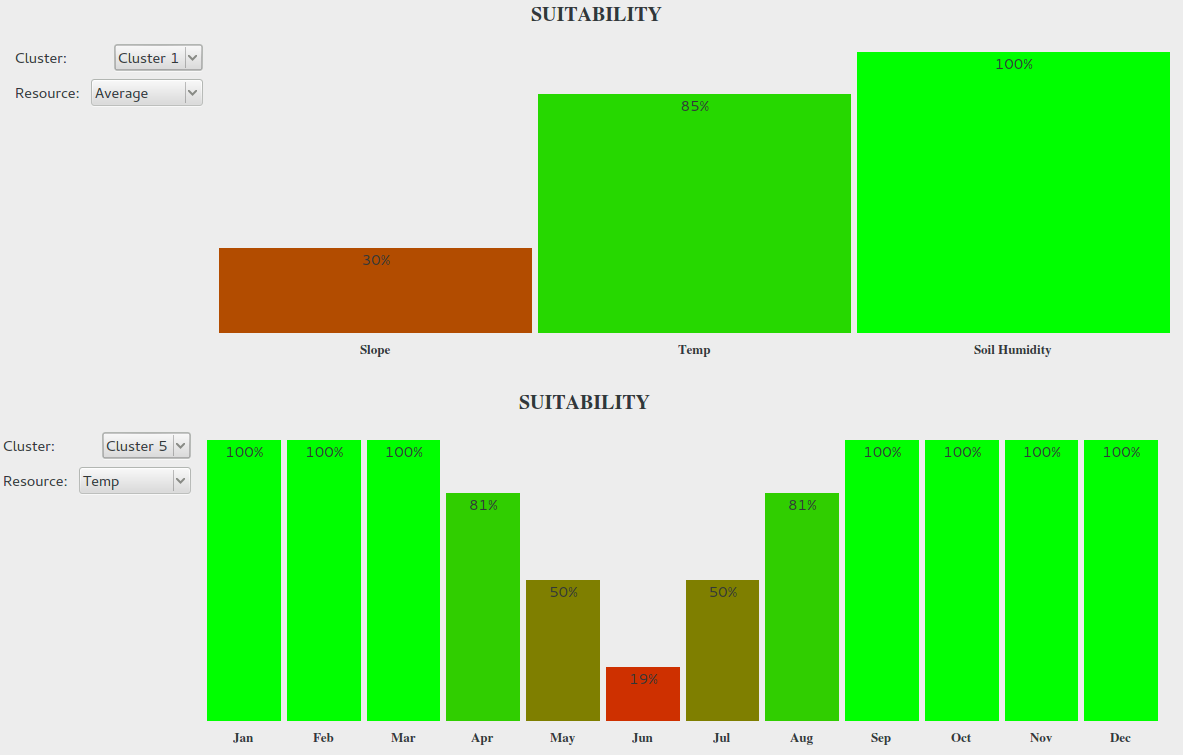
\includegraphics[width=\textwidth]{specie_suitability_temp_and_avg.png}
	\caption{ Overall (top) and temperature (bottom) intermediate species suitability histograms. Not displayed but also is the humidity intermediate species suitability histograms.}	
	\label{fig:specie_intermediate_suitability_scores}
\end{figure}



\section{Ecosystem Simulator} \label{sec:ecosystem_simulator}

Once the user selects the union of all species to appear in all clusters of the terrain, it is necessary to determine a valid vegetation distribution for each. To do so, an ecosystem simulator is used as in the work of Deussen et al \cite{Deussen1998} and Lane and Przemyslaw \cite{Lane2002}. Unlike these other ecosystem simulators, however, our approach is not based on L-Systems, and models both resource requirements and resource availability in greater detail. The purpose of the ecosystem simulator is to determine, given a vegetation state, \textit{S$_{t}$} at time \textit{t}, the state \textit{S$_{t+n}$} at time \textit{t+n}, for any value of n. To do so, the simulation advances through time at monthly intervals and the strength of all plant instances are iteratively re-calculated. This strength of a given plant depends on it's age, available resources and surrounding plants with which it is competing for resources. This calculated value directly influences the plants growth and ability to survive.\\

\subsection{Gridded Simulation Area}

The simulation area greatly effects the performance of the ecosystem simulator and, therefore, it is necessary to keep it to a minimum. However, too small a simulation area will fail to accurately model the interaction of larger plant species. Given these constraints, a simulation window of one hundred by one hundred meters is used, accurate to the nearest centimetre. This area is deemed conservative, however, as rare are the species which come remotely close to such spatial coverage. An extension to this work would be to adjust the size of the simulation window depending on the  species selected. This would ensure optimal simulation speed for all simulation runs. \\

When iteratively calculating the strength of plant instances, it is necessary to quickly determine the set of plants S = \{P$_{1}$, P$_{2}$, P$_{3}$, ...\} competing for available resources with \textit{P$_{n}$}. Determining \textit{S} depends on the spatial reach of \textit{P$_{n}$}. Spatial awareness is therefore a key requirement of the simulation and is achieved by splitting the simulation window into a grid of smaller cells. \\

The size of individual cells can be configured to increase or decrease the resolution and, therefore, the accuracy of the simulation. As the simulation progresses, plants grow, their spatial coverage increases, and they enter new grid cells. When a plant enters a new grid cell, it becomes a member and cell resources are distributed to it. The information associated with each individual grid cell can be split into two categories: \textit{time-dependent} and \textit{simulation-dependent}. The time-dependent information depends only on the current month, is identical for every grid cell and comprised of: the \textit{soil moisture} and the \textit{illumination}. The simulation-dependent information varies throughout the simulation as plants spawn, die and grow and consists of: the \textit{list of plants whose roots intersect the cell} and the \textit{list of plants whose canopy intersects the cell}. It is important to have both as plant roots and canopies grow at different rates and their cell coverage will therefore differ. \\
By employing this gridded approach, determining the set of plants which compete for resources is extremely efficient. For example, to determine the set of plants with which \textit{P$_{n}$} is competing for soil moisture, it is only necessary to determine the cells covered by its roots, which depends solely on its position and root size.\\
Another advantage of this gridded approach, which is discussed in further detail below, is that it splits plants into separate cells, each with unique resource distributions. This permits partial shading, for example, where illumination is zero in some of its cells but more in others. \\

\subsection{Soil Moisture Distribution} \label{subsec:humidity_distribution}

Plants grow their roots in order to access the nutrients and moisture available in the surrounding soil. As roots of different plant instances overlap, they compete for these resources. A notable simplification in our work is that soil depth is not modelled. Soil depth affects the plants rooting reach and has a significant impact on plant growth \cite{Fourcaud2008}. A a future extension to this work, the soil could be modelled as layers, which would permit plants to battle for different soil resources depending on their root depth. For example, grass and shrub with small root depth would access soil moisture in the upper most layer but large trees would access it in the deeper most layer. They would therefore not be competing for soil moisture. \\

The strength of each plant in the simulation must be recalculated on a monthly basis. Part of the information required to calculate the overall strength of a given plant is the moisture allocated to it, which is taken as the average of the moisture allocated to it in each cell its roots overlap. To determine the overall moisture allocated to a given plant \textit{p}, it is first necessary, therefore, to iterate over all incident grid cells and calculate the moisture allocated to each plant with intersecting roots.\\

When distributing the soil moisture in a given grid cell \textit{C$_{xy}$} to the set \textit{S} = \{P$_{1}$, P$_{2}$, P$_{3}$, ...\} of plants whose roots intersect the cell, one of three distinct scenarios can occur, depending on the available moisture, \textit{M$_{available}$}, of the cell: \textit{Abundant}, \textit{sufficient} and \textit{insufficient}.\\

The moisture is deemed abundant if the available moisture, \textit{M$_{available}$}, surpasses 300 millimetres. To prevent situations where the soil moisture attributed to a given plant is small simply because the majority of the available moisture is distributed to other plants, all plants of \textit{S} are allocated \textit{M$_{available}$}. This is important as it could lead to situations where species strive in areas completely unsuited. The available soil moisture is directly dependent on rainfall. At three hundred millimetres, rainfall can be considered abundant and soil moisture therefore not a limiting factor. \\

If \textit{M$_{available}$} is less than 300 millimetres, it is necessary to determine whether the moisture is sufficient or insufficient by calculating the requested moisture \textit{M$_{requested}$}, as outlined in equation \ref{eq:humidity_requested_calc}. \\

\begin{equation}
M_{requested} = \sum MinMoisture(P_{n}) \text{ for } n \in S
\label{eq:humidity_requested_calc}
\end{equation}
Where: \textit{MinMoisture(P$_{n}$)} is the minimum moisture requirement of the species to which plant \textit{P$_{n}$} belongs; \textit{S} is the set of plants whose roots intersect the given grid cell.\\

If \textit{M$_{requested}$} is less than \textit{M$_{available}$}, the moisture is deemed sufficient and the amount allocated to each plant is calculated as described in equation \ref{eq:humidity_allocation_sufficient_calc}. Intuitively, this equation allocates each plant with the minimum amount of humidity it requires to survive plus the resulting overflow. Note that in this equation, the overflow is not distributed amongst plants of the cell but rather allocated to each plant. For the same reason as to why all plants are allocated \textit{M$_{available}$} when it is deemed abundant, it is to prevent situation where unsuited plant species are able to grow because the moisture allocated to it is low simply because it is distributed to other plants.\\

\begin{equation}
\begin{split}
M_{allocated}(P_{n}) = MinMoisture(P_{n}) + OverFlow \\
OverFlow = M_{available} - \sum MinMoisture(P_{n}) \text{ for } n \in S
\end{split}
\label{eq:humidity_allocation_sufficient_calc}
\end{equation}
Where: \textit{M$_{allocated}$(P$_{n}$)} is the humidity allocated to plant \textit{P$_{n}$};\\

If \textit{M$_{requested}$} is more than \textit{M$_{available}$}, however, the humidity is deemed insufficient and the allocation follows algorithm \ref{alg:humidity_allocation_insufficient_calc} which prioritises water distribution to the more vigorous plants. The vigour of a plant is estimated based on its root size. This ensures stronger plants have better access to water than smaller, weaker ones.\\

\begin{algorithm}
\caption{Algorithm to distribute soil moisture within a cell when the quantity is insufficient.}
\begin{algorithmic}[1]
\REQUIRE Initialize $S_{remaining}$ as the total moisture available in the cell.
\REQUIRE Initialize $S$ as the set of all plants whose roots intersect the cell, sorted in decreasing order of root size
\STATE TotalRootSize = 0
\FOR{$P_{n}$ in $S$}
	\STATE TotalRootSize += RootSize($P_{n}$)
\ENDFOR
\FOR{$P_{n}$ in $S$}
	\STATE Vigour = $\frac{RootSize(P_{n})}{\sum RootSize(P_{x}) \text{ for } x \in S}$\\
	\STATE M$_{allocated}(P_{n})$ = $min(MinMoisture(P_{n}), Vigour \times M_{remaining})$ \\
	\STATE M$_{remaining}$ -= M$_{allocated}$
	\STATE Remove $P_{n}$ from the set S
\ENDFOR
\end{algorithmic}
\label{alg:humidity_allocation_insufficient_calc}
\end{algorithm}

The overall moisture allocated to \textit{P$_{n}$} is calculated using equation \ref{eq:plant_humidity_allocation}. Intuitively, it is simply the average of all moisture allocated to it within all cells of \textit{S}.

\begin{equation}
M_{n} = \frac{\sum M_{allocated}(C_{x}) \text{ for } x \in S}{| S |}
\label{eq:plant_humidity_allocation}
\end{equation}
Where:\textit{M$_{n}$} is the moisture allocated to plant \textit{P$_{n}$}; \textit{M$_{allocated}$(C$_{n}$)} is the moisture allocated to plant \textit{P$_{n}$} in grid cell C$_{n}$; \textit{$|$ S $|$} is the number of cells in the set \textit{S}.\\

\subsection{Illumination Distribution}

Photosynthesis is an essential part of plant development as it permits the creation of fresh matter and, therefore, growth \cite{Soler2001}. Species that are heavily dependent on illumination will often grow large canopies to maximize the leaf coverage area and therefore photosynthesis potential. These large canopies also limit the illumination available in the area underneath the canopy, limiting plant development. To model this, available illumination is calculated for each grid cell based on the height of the plants with canopies intersecting the given cell, as outlined in equation \ref{eq:illum_distribution}. Intuitively, if all plants present in the given cell are canopy-free, the equation allocates them all the available illumination. If not, the equation allocates illumination only to the tallest canopy plant. A canopy-free plant is one which grows more in height than width and for which shade projection can be ignored (e.g grass, cacti, etc.). Note that this is a simplification as some light should still pass through the canopy and the shade projected by the canopy does not always fall directly below but varies throughout the day and the year. A much more detailed approach is taken by Soler et al. \cite{Soler2001}, who model light transmittance through the canopy based on plant geometry. This detailed approach is ill-suited here, however, as the growth of a large set of plants needs to be simulated simultaneously. A possible extension to this work would be to associate with each plant species a canopy density parameter, which affects the quantity of light which can pass through its canopy.

\begin{equation}
\centering
Illumination(C_{xy}, P_{n}) = 
\begin{cases}
	C_{illumination}, & \text{if } CanopyWidth(P) = 0 for P \in S \\
	C_{illumination}, & \text{if } Height(P_{n}) > height(P) for P \in S : P \neq P_{n} \\
    0,              & \text{otherwise}
\end{cases}
\label{eq:illum_distribution}
\end{equation}
Where: \textit{Illumination($C_{xy},P_{n}$)} is the illumination allocated to plant \textit{P$_{n}$} whose canopy overlaps grid cell C$_{xy}$; \textit{C$_{illumination}$} is the available illumination for the given month (equal for all cells);\textit{CanopyWidth(P)} is the canopy width of plant \textit{P}; \textit{Height(P)} is the height of plant \textit{P}; \textit{S} is the set of plants whose canopy intersects with the given grid cell \textit{C$_{xy}$}.\\

Calculating the illumination allocated to a plant \textit{P$_{n}$} is identical to calculating the humidity allocated (see equation \ref{eq:plant_humidity_allocation}) but the cells considered are those which the plants canopy intersects (and not its roots). Intuitively, the illumination allocated to a given plant is simply the average of the illumination allocated to it in all grid cells its canopy intersect.\\

By calculating the illumination separately for each cell covered by a plants canopy and then taking the average as the aggregate illumination, it is possible to model partial shade. For example, if half the grid cells covered by a plants canopy are shaded (zero illumination) and the other half receive ten hours of daily illumination, the aggregate would be five hours.\\

\subsection{Plant Strength Calculation} \label{subsec:plant_strength_calc}

Given the humidity and illumination allocated to a given plant \textit{P}, the temperature, the slope and the age of \textit{P}, it is possible to calculate its overall strength (vigour), which is subsequently used as a representation of the plants health and directly affects its growth and survival. \\
The overall strength, of plant \textit{P}, is taken as the minimum of \textit{S$_{slope}$}, \textit{S$_{age}$}, \textit{S$_{temperature}$}, \textit{S$_{illumination}$} and \textit{S$_{humidity}$}, which represent the strength of \textit{P} in terms of the slope, its age, the temperature, the allocated illumination and humidity, respectively. The minimum is taken rather than the average as the strength of a plant depends heavily which resource is limiting. For example, if a plant is struggling due to a lack of daily illumination, improving the allocated water would not have a big impact on its overall health.\\
To calculate the individual strength values, in the range [-100,100], a graph is plotted as outlined in figures \ref{fig:2_value_strength} and \ref{fig:4_value_strength} for each species. These graphs are generate for each resource based on the associated properties (see section \ref{sec:plant_species}). Using these, it is possible to calculate the plants strength in terms of slope, age, temperature, illumination and humidity. When a plant has a negative strength it is deemed in \textit{survival}. When in this state, it does not grow and is susceptible to be killed off.\\

\begin{figure}
\center
	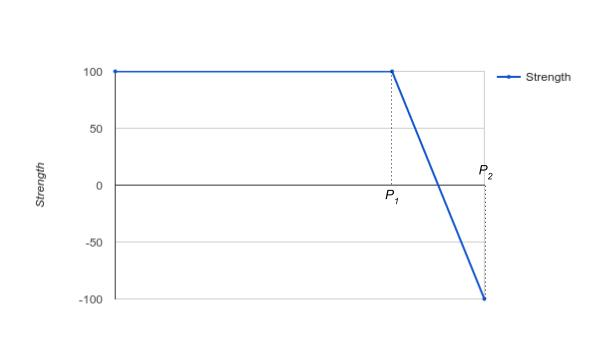
\includegraphics[scale=0.7]{2_value_strength.jpg}
	\caption{ \textit{Graph used to calculate the slope and age strength of a given plant instance where: \textbf{P$_{1}$} represents the value of \textit{start of decline} and \textbf{P$_{2}$} is the \textit{maximum} configured for the given species.} }	
	\label{fig:2_value_strength}
\end{figure}

\begin{figure}
\center
	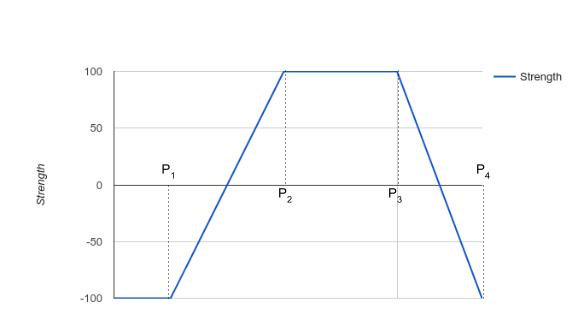
\includegraphics[scale=0.7]{4_value_strength.jpg}
	\caption{ \textit{Graph used to calculate the temperature, illumination and humidity strength of a given plant instance where: \textbf{P$_{1}$} and \textbf{P$_{4}$} are the \textit{minimum} and \textit{maximum} and \textbf{P$_{2}$} and \textbf{P$_{3}$} form the \textit{prime range} configured for the given species.}  }	
	\label{fig:4_value_strength}
\end{figure}

\subsection{Plant Growth}

In the simulation, each plant \textit{P} attempts to grow its roots, its canopy and its height on a monthly basis. Each species has a maximum monthly root growth, canopy growth and height growth which are calculated as outlined in equation \ref{eq:max_growth}. The maximum height, canopy and root size, along with the species age-based start of decline (see section \ref{sec:plant_species}) are used to calculate the amount it must grow each month to reach these maximums by start of decline. Note that this is a simplification as, in reality, plant growth is non-linear as growth slows with increasing size \cite{Paine2012}.

\begin{equation}
MaxGrowth(S) = \frac{Max(S)}{Age_{sod}(S)}
\label{eq:max_growth}
\end{equation}
Where:\textit{MaxGrowth(S)} is the maximum monthly root, canopy or height growth of species \textit{S}; \textit{Max(S)} is the maximum root size, canopy size or height configured for species \textit{S}; \textit{Age$_{sod}$(S)} is the age of start of decline configured for species \textit{S}.\\

The actual root growth, canopy growth and height growth of a plant is directly dependent on its strength (see section \ref{subsec:plant_strength_calc}), however, and is calculated using equation \ref{eq:actual_growth}. This equation only permits growth if the plants strength is positive as it is otherwise deemed too weak to grow and in a state of \textit{survival}. If the strength is positive, the growth is proportional to the plants strength. The maximum growth is therefore only achieved if the plant is at full strength.\\

\begin{equation}
Growth(\textit{P},S) = max(0, Strength(\textit{P}) \times  MaxGrowth(S)
\label{eq:actual_growth}
\end{equation}
Where: \textit{Growth(S)} is the monthly root, canopy or height growth of plant \textit{P} of species \textit{S}; \textit{Strength(P)} is the current strength of \textit{P}; \textit{MaxGrowth(S)} is the maximum monthly root, canopy or height growth calculated for species \textit{S} (see equation \ref{eq:max_growth}).

\subsection{Plant Death}

In order for the simulation to be accurate, it is necessary to model plant death. This can be caused by ageing, the slope being ill-suited or resources being inadequate. On a monthly basis, the probability of death of each plant is calculated based on its strength using equation \ref{eq:probability_of_death} and the plant killed off with the given probability. This equation permits plants to be killed-off only when in a survival state (i.e the strength is negative). If this is the case, the probability of death is proportional to the absolute value of the strength. 

\begin{equation}
Probability_{death}(P) = max(0, \frac{-1 \times Strength(P) + counter}{100})
\label{eq:probability_of_death}
\end{equation}
Where:\textit{Probability{death}(P)} is the probability of death of plant \textit{P};\textit{counter} is a value which increases each month the plants strength is negative, and resets to zero when it becomes positive. This prevents plants from surviving in a survival state for too long.

\subsection{Spawning Plants} \label{subsec:spawning_plants}

In nature, the spawning of new plants ensures species \textit{succession} and \textit{propagation}. In order to accurately model the evolution of an ecosystem it is essential to replicate this spawning mechanism. To do so, seeds are produced annually for each species and are positioned either randomly or at predefined positions. The number of seeds that are produced for a given species is determined by the species configured \textit{annual seed count}. Different seeding mechanisms are used in the simulator depending on the current state of the simulation, as discussed below.\\ 

To ensure species propagation, when plants of the given species are already present in the simulation window, they are used to determine the location for new plant instances. To do so, \textit{n} of these plants are selected at random and seeds placed at random within an annular radius \textit{r} of each. The value of \textit{n} is the \textit{annual seed count} configured for the current specie. The value of \textit{r} is the configured \textit{maximum seeding distance} of the specie. Note that a single plant can be used to spawn multiple seeds if \textit{n} is greater than the number of plants of the given species present in the simulation.\\
This technique is effective in ensuring \textit{propagation} until the number of plant instances present far outweighs the number of seeds, at which point, the \textit{propagation} potential decreases. This is because, as the selection pool for the random seeding plants increases in size, the probability of selecting a seeding plant at a location which will permit propagation decreases. For example, if there are 100 plants of species \textit{s} within a 2 metre square window and 50 are selected for seeding, there is a high probability that a number of them will be selected at the extremities and, therefore, propagate the species further. If there are 10000 plants of the given species, however, the probability of selecting extremity plants and is very low. To overcome this and ensure the initial seeding plants that are selected span a wide area, the simulation window is split into equally sized cells and the seeding plants selected individually from each. \\

If no instance of the given species is present in the simulation (i.e it is the first month) and therefore no seeding plants can be used, the seeds are placed at random within the simulation window.\\ 

A species is deemed shade-loving if its configured minimum daily illumination is zero. Such species thrive in the undergrowth of other plants. Spawning shade-loving species in the same way as other plants would drastically limit their chance of survival because the probability of a random seed location falling in the canopy of an existing plant is very low. For this reason, when there are no instances of the given shade-loving species present in the simulation window, the seed locations are located at random under the canopy of existing plants. If instances of the plant species are already present, however, they are used to propagate the seeds, just like with other, non shade-loving, plant species.

\subsection{Performance} \label{subsec:ecosytem_performance}

The number of plants present in the simulation will heavily influence its performance as the strength of each plant needs to be recalculated on a monthly basis. To test the influence of plant count on simulation execution time, a simulation is run with a single species of plant and the monthly processing time analysed alongside the number of plants present. The plant used is grass as is has no canopy and very minimal root coverage, therefore permitting a large number of instances to grow simultaneously (see appendix \ref{AppendixB} for properties of the specie). The resources were set to be optimal for maximizing plant count and minimizing intra-plant competition. The simulation is started with only a single instance and, as the simulation progresses and seeding is performed, the number of instances increases. The results are summarized in Figure \ref{fig:ecosimulator_test_plant_count} and show that the processing time increases linearly with plant count. The jump at the 65 thousand plant mark occurred repeatedly over multiple tests. Although just a hypothesise, the most likely cause is that it is a tipping point at which page swapping starts to occur due to saturated RAM.\\

\begin{figure}
\center
	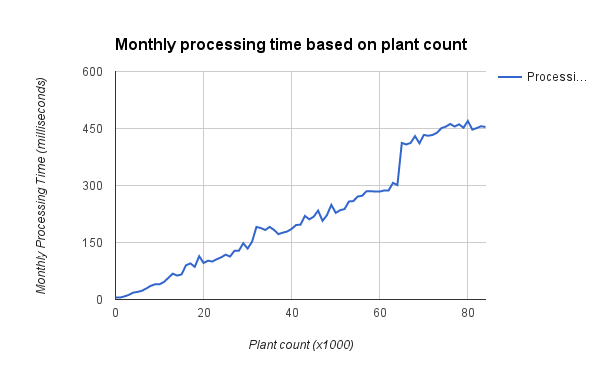
\includegraphics[scale=0.7]{ecosimulator_test_plant_count.png}
	\caption{ \textit{Processing time based on plant count. Total simulation time for 100 years: 271 seconds}}	
	\label{fig:ecosimulator_test_plant_count}
\end{figure}

Another property that heavily impacts performance is the root and canopy growth. As roots and canopies grow, they will cover more grid cells of the simulation window, and more calculations will be required per individual cell. To analyse the impact of plant growth, a base species \textit{S$_{base}$} is created with a given root and canopy growth rate. Then, two species \textit{S$_{X2}$} and \textit{S$_{X3}$} are created with identical properties to \textit{S$_{base}$} but with twice and thrice the growth rates, respectively (see appendix \ref{AppendixB} for species details). Separate simulations are run with each species but with identical available resources and, on a monthly basis, the number of plants present in the simulation, along with the monthly processing time, are analysed. Given this information, it is possible to track the average monthly execution time per plant throughout the simulation. It is important to normalise this based on the number of plants as faster growing plants will naturally reduce the total plant count for the simple reason that they will require and be able to access resources from a larger number of grid cells. As can be seen in the results plotted in figure \ref{fig:ecosimulator_test_per_plant}, the processing times are similar to begin with and then increase proportionally to the species growth rate. For the fastest growing plant specie, \textit{S$_{X3}$}, it took 166 seconds to simulate one hundred years.

\begin{figure}
\center
	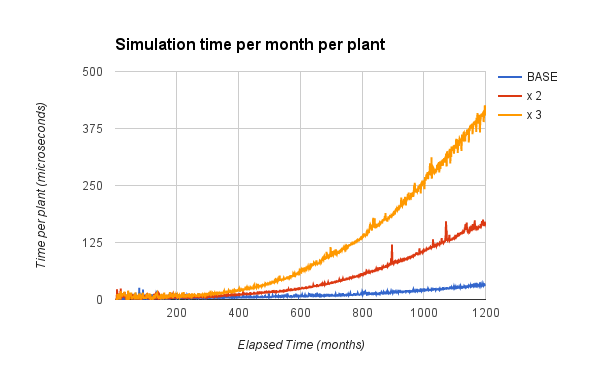
\includegraphics[scale=0.7]{ecosimulator_test_per_plant.png}
	\caption{ \textit{Evolution of the monthly processing time normalised based on plant count. The processing time increases as the plants grow larger since they cover more grid cells. Total simulation time for one hundred years: ~49 seconds for \textit{S$_{base}$}, ~122 seconds for \textit{S$_{X2}$} and 166 seconds for \textit{S$_{X3}$}}}
	\label{fig:ecosimulator_test_per_plant}
\end{figure}

\subsection{Results} \label{subsec:ecosystem_simulator_results}

To test the resulting spatial distribution of plant communities in their work, Lane and Przemyslaw \cite{Lane2002} attempt to reproduce three important properties of nature: \textit{Self-thinning}, \textit{succession} and \textit{propagation}. To test the ecosystem simulator, we employ the same methodology as Lane and and Przemyslaw \cite{Lane2002} and attempt to reproduce these core properties of nature. Other tests are also performed to ensure plant instances thrive better in environments suited to their individual resource requirements.\\

\textbf{SELF-THINNING TEST}\\

As plants grow, their resource requirements increase and, as a direct consequence, inter-plant competition for resources increases. Eventually, the competition becomes too intense and resources too scarce, leading to more vigorous plants starving smaller plants. At this point, \textit{self-thinning} begins and plant densities decrease \cite{Lane2002}.\\
To test whether self-thinning is successfully modelled in the ecosystem simulator, three simulations are run differing only in the configured soil moisture and the plant count tracked throughout. As described previously, self-thinning occurs because of insufficient resources. By modifying only available humidity in each simulation, its affect on self-thinning becomes apparent. As can be seen in the results summarized in figure \ref{fig:self_thinning_test_results}, the plant count increases at first, reaches a maximum and decreases thereafter. This is the expected behaviour of self-thinning. Furthermore, it is apparent that the maximum plant count increases with the humidity available, therefore showing that the tipping point depends on available resources.\\

\begin{figure}
\center
	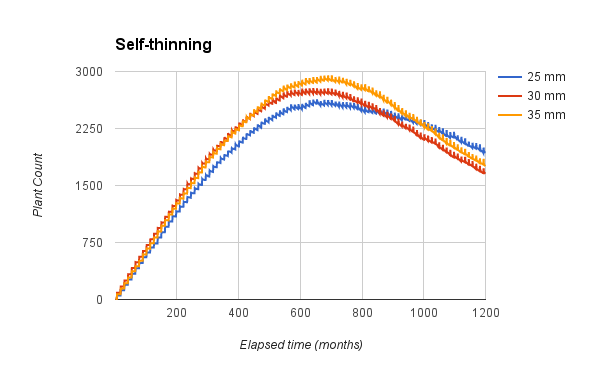
\includegraphics[scale=0.7]{self_thinning.png}
	\caption{ \textit{Self thinning test: plant count tracked throughout three separate simulations differing only in available humidity. For all three runs the plant density reaches a maximum tipping-point after which plant density reduces. Note that the more available moisture there is, the more severe the slope of descent is following the tipping point. This is because, with more soil moisture available, plants thrive and reach greater sizes. Because of this increased spatial coverage, the killing off of smaller plants is more severe. So, although the plant count is smaller by the end of the simulations when there is more humidity, the average plant size is larger.}}
	\label{fig:self_thinning_test_results}
\end{figure}

\textbf{SUCCESSION TEST}\\

Given plant species \textit{A} with a fast growth rate and species \textit{B} with a slower growth rate but higher shade tolerance. At first, the faster growing species A will dominate and flourish but, with time, the slower growing, but more shade-tolerant species B will flourish and dominate. This is the \textit{succession} property. To test \textit{succession} in the ecosystem simulator, two plant species \textit{S$_{fast}$} and \textit{S$_{slow}$} are created differing only in their growth rate and illumination properties (see appendix \ref{AppendixB} for details) and a simulation run with these two species under optimal conditions. During the simulation, the appearance and average size of the two plant species are monitored to determine the dominating specie. The results are analysed and illustrated in figure \ref{fig:succession_plants_avg_size}. A snapshot of the simulation window is taken at ten year intervals and displayed in figure \ref{fig:succession_plants_render}. Both these figures show that \textit{S$_{fast}$} dominates at first (~300 months in) followed by \textit{S$_{slow}$} (~500 months in). A balance is found thereafter.\\

\begin{figure}
\center
	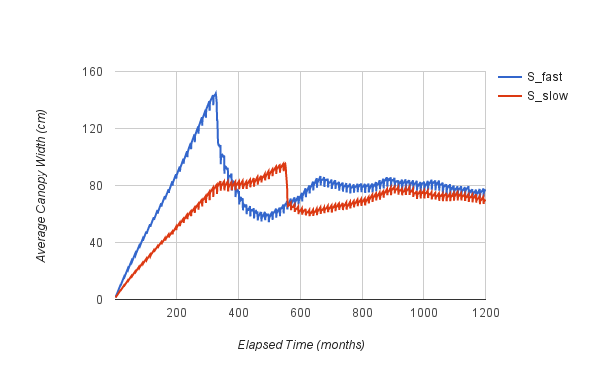
\includegraphics[scale=0.7]{succession_plant_avg_size.png}
	\caption{ \textit{Succession Test: Average size of the slow growing S$_{slow}$ (red) and fast growing S$_{fast}$ (blue) throughout a simulation run in optimal conditions. Note that the plant count drops severely at the 300 and 500 mark for S$_{fast}$ and S$_{slow}$ respectively as resources are configured such that conditions are ideal for these species. This leads to a large quantity of them dying of age and, because the difference between start of decline and maximum age configured for these species is very small, it is done performed very sharply.}}
	\label{fig:succession_plants_avg_size}
\end{figure}

\begin{figure}
\center
	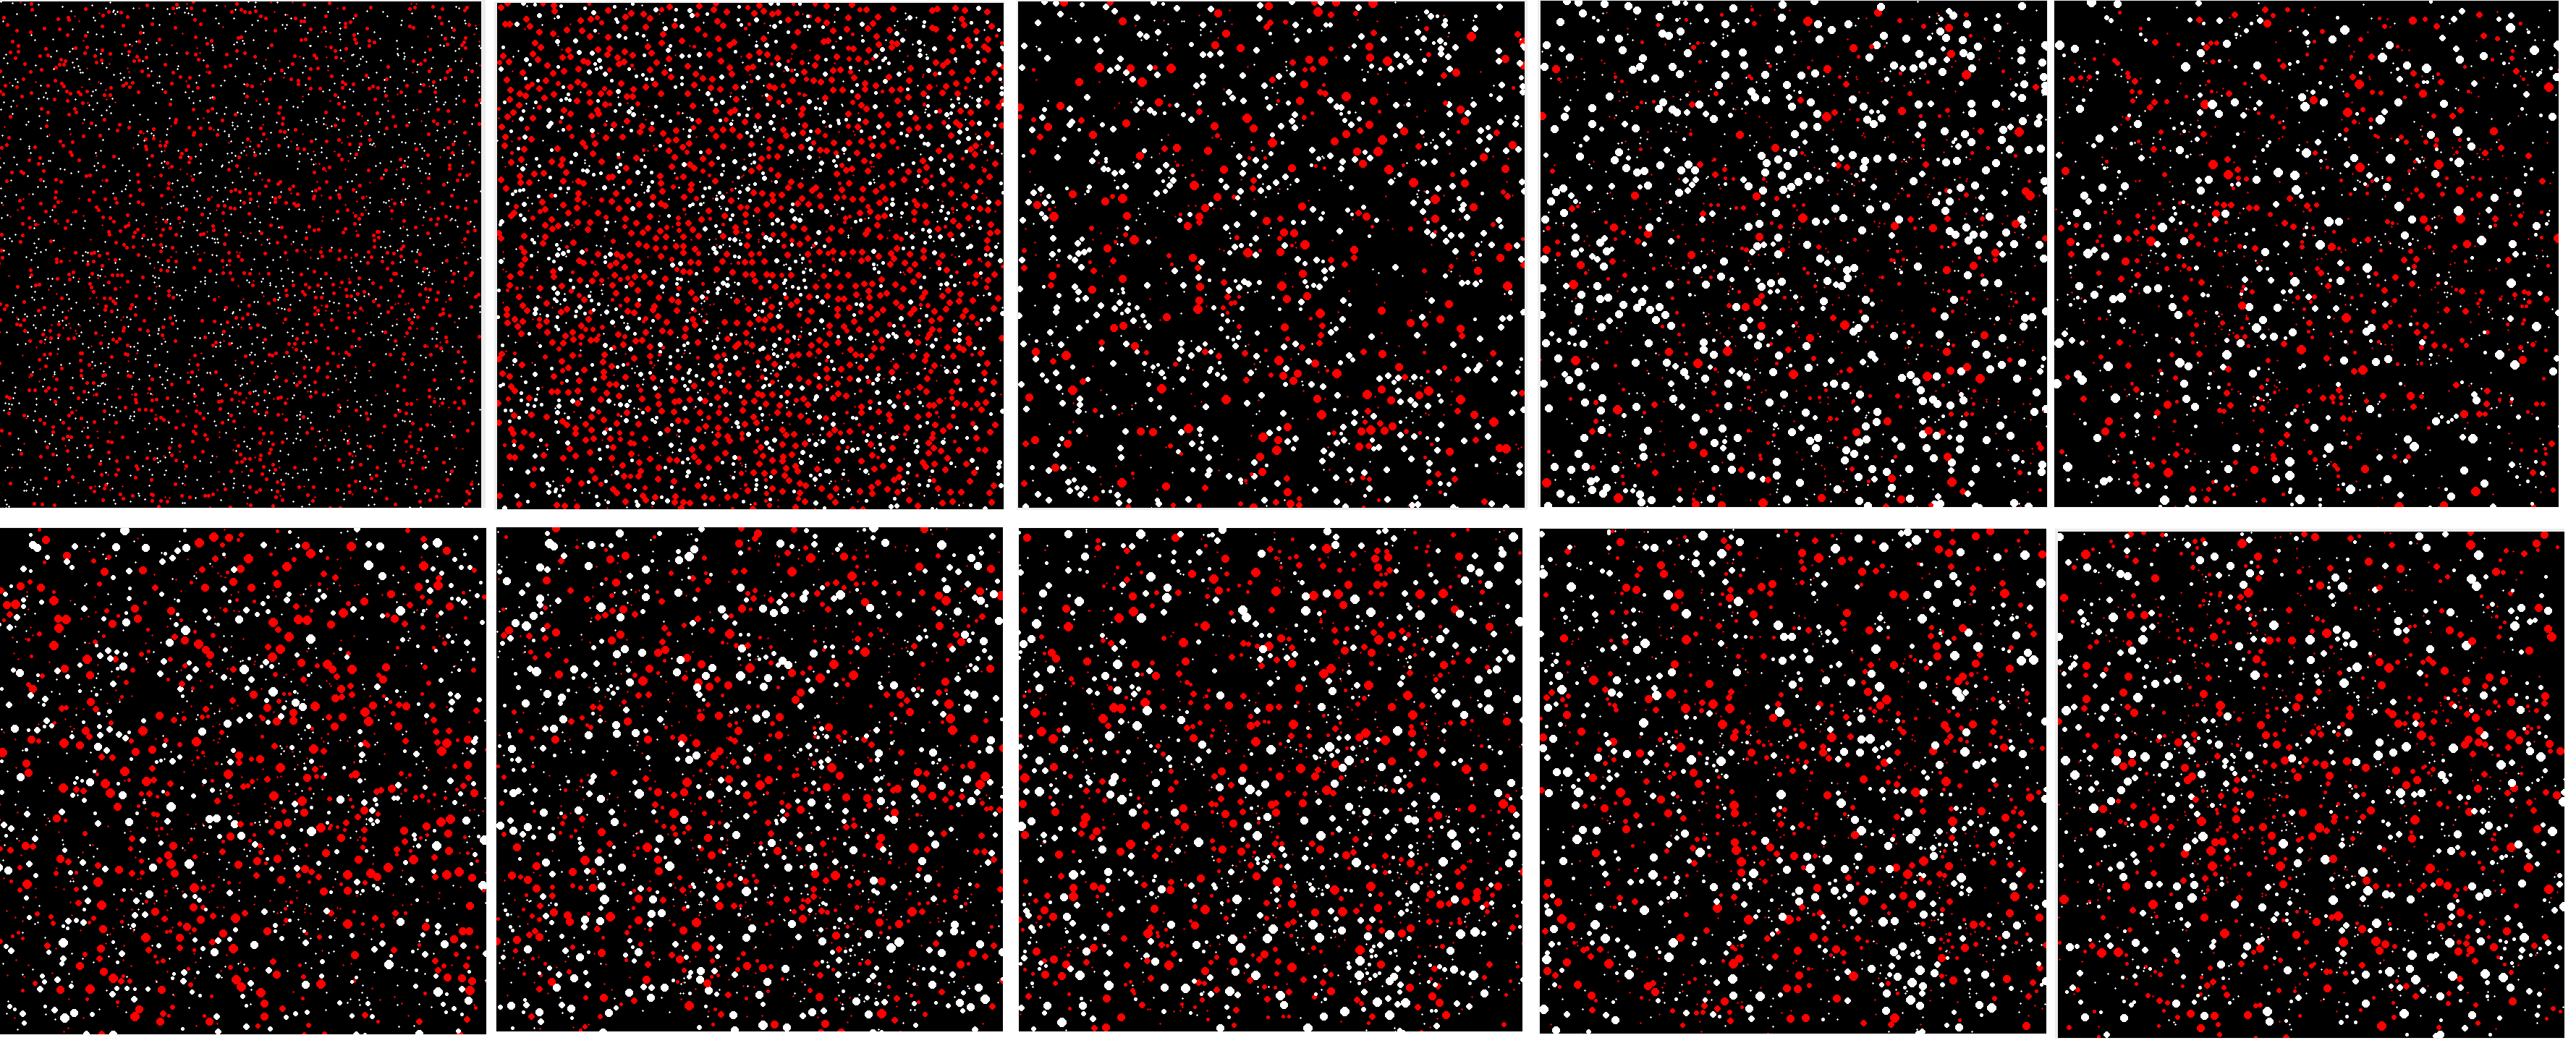
\includegraphics[width=\textwidth]{succession_plants_render.png}
	\caption{ \textit{Succession Test: Appearance of the slow growing S$_{slow}$ (white) and fast growing S$_{fast}$ (red) at different times during the simulation. From left-to-right, top-top-bottom: 10, 20, 30, 40, 50, 60, 70, 80, 90 and 100 years.}}
	\label{fig:succession_plants_render}
\end{figure}

\textbf{PROPAGATION TEST}\\

The \textit{propagation} property simply states that plants \textit{propagate} in clusters surrounding the seed plants. To ensure propagation is modelled, a simulation is run with a single starting grass seed (see appendix \ref{AppendixB} for species details) and its evolution tracked throughout. Figure \ref{fig:propagation_test_render} shows that iterative propagation through annual seeding enables a single seed plant to colonize the entirety of the terrain. Note that, although it does show propagation is reproduced, it is unrealistically slow. This is caused by the seeding algorithm used. As discussed in section \ref{subsec:spawning_plants}, in order to promote propagation, the simulation window is split into grids and seeding plants selected separately from each cell. Although this increases the spatial coverage of the seeding plants, it still fails to propagate effectively when the number of grid cells in which the given species appears is large as the probability of selecting a grid cell from the edge (which would lead to seeding) decreases with the grid coverage of the given specie. A worthwhile extension to this work would be to implement the ability to locate border grid cells and use them more extensively during seeding. This could be done by, for example, sorting the grid cells in order of the species count they contain as border cells would naturally be less dense. \\

\begin{figure}
\center
	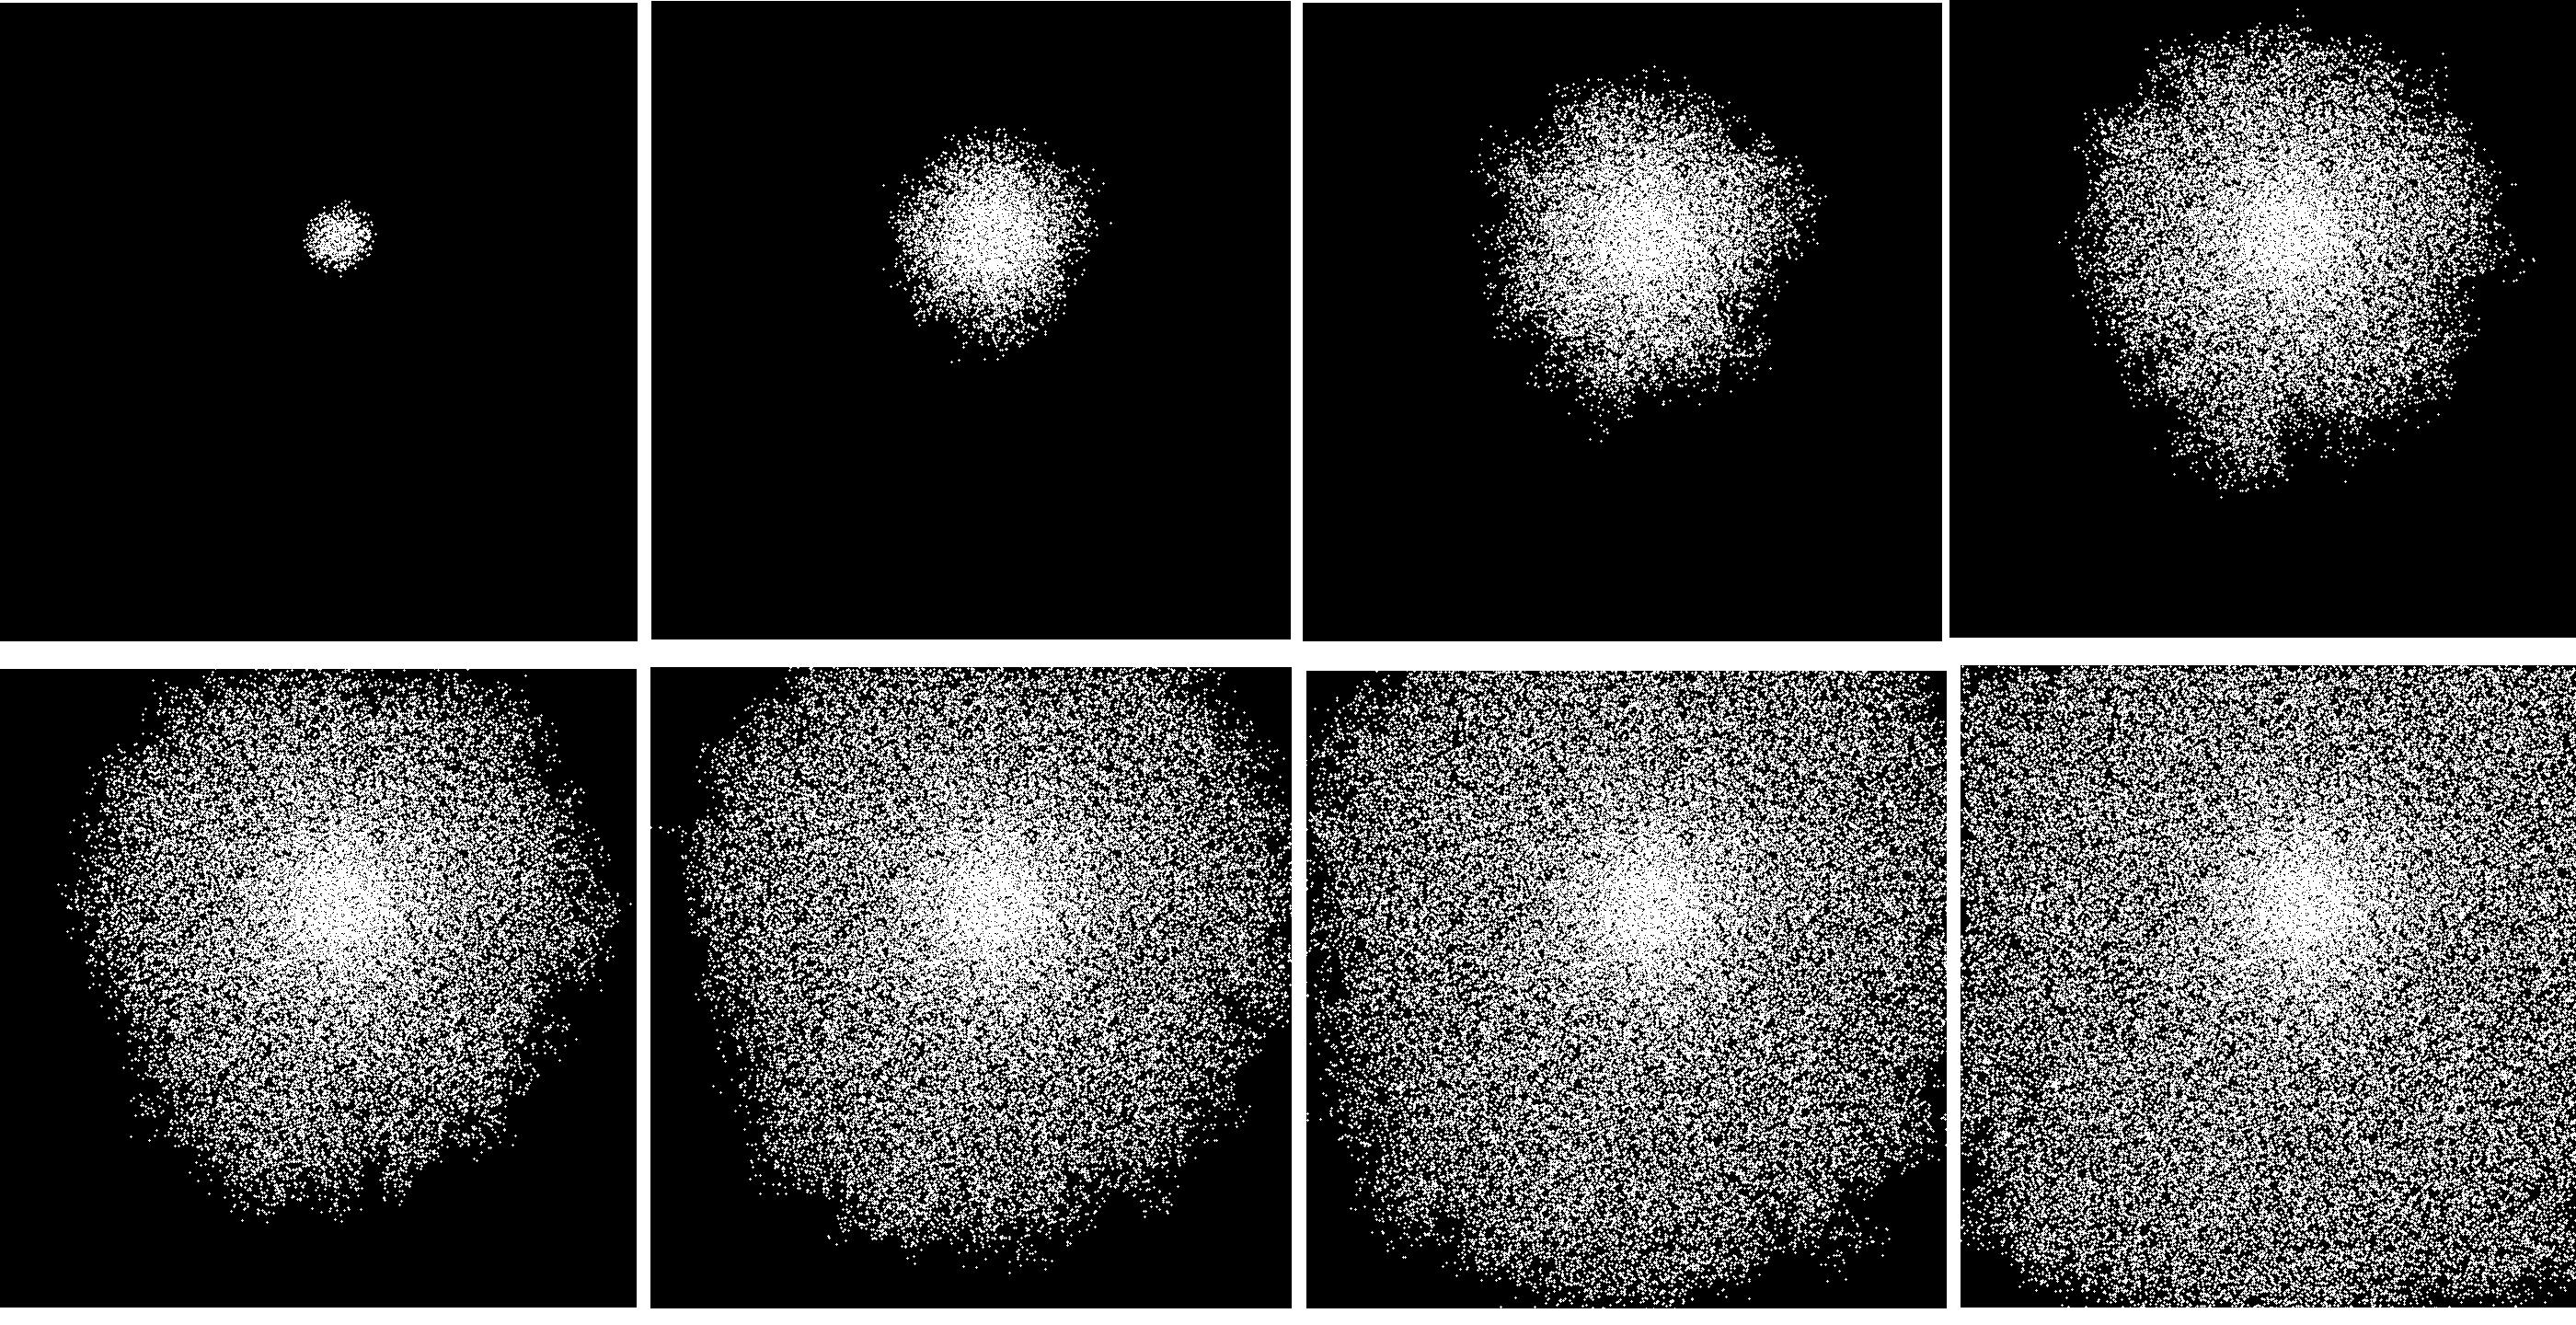
\includegraphics[width=\textwidth]{propagation_test_render.png}
	\caption{ \textit{Propagation Test: Evolution through time of a simulation starting from a single seed plant of grass. From left-to-right, top-to-bottom: 2, 10, 20, 30, 40, 50, 60, 70 years in.}}
	\label{fig:propagation_test_render}
\end{figure}

\textbf{VARYING RESOURCE TEST} \\

To ensure a given plant species thrives better when the environment is more suitable, multiple simulations are run with a single species \textit{S$_{base}$} (see appendix \ref{AppendixB} for species properties) varying only in available humidity. Throughout the simulation, the average plant canopy width is tracked to monitor the strength of the plants. As can be seen by the results plotted in figure \ref{fig:varying_resource_test}, plants thrive better in environments better suited to their resource requirements.\\

\begin{figure}
\center
	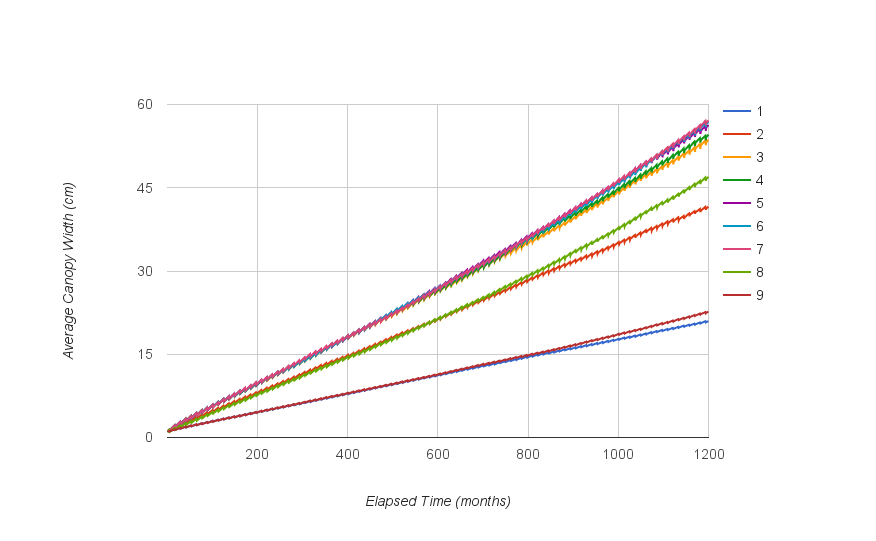
\includegraphics[width=\textwidth]{varying_resource_test.png}
	\caption{ \textit{Varying resource test: Average canopy width throughout simulations varying only in available moisture and with only plant species \textit{S$_{base}$}. It shows that the average canopy width is low when the configured humidity is outside the species optimal humidity range (22mm and 38mm), improves as it approaches optimal range (24mm and 36mm) and reaches its peak when the humidity is within the optimal range (26mmn, 28mm, 30mm, 32mm and 34mm).}}
	\label{fig:varying_resource_test}
\end{figure}

\textbf{SHADE TEST}\\

Plants that are heavily dependent on illumination struggle to grow in areas shaded by the canopy of larger plants. To ensure this is modelled in the ecosystem simulator, a simulation is run with two species: \textit{S$_{smallroots}$} and grass (see appendix \ref{AppendixB} for species details). \textit{S$_{smallroots}$} is a custom species created for the purpose of this test which has a very small root growth value. This is important so as to focus on the effects of illumination and minimize the influence of drought. Figure \ref{fig:shade_test}, which illustrates the state of the simulation after ten years, shows the grass struggling to grow in areas directly below the canopies of \textit{S$_{smallroots}$}.\\

\begin{figure}
\center
	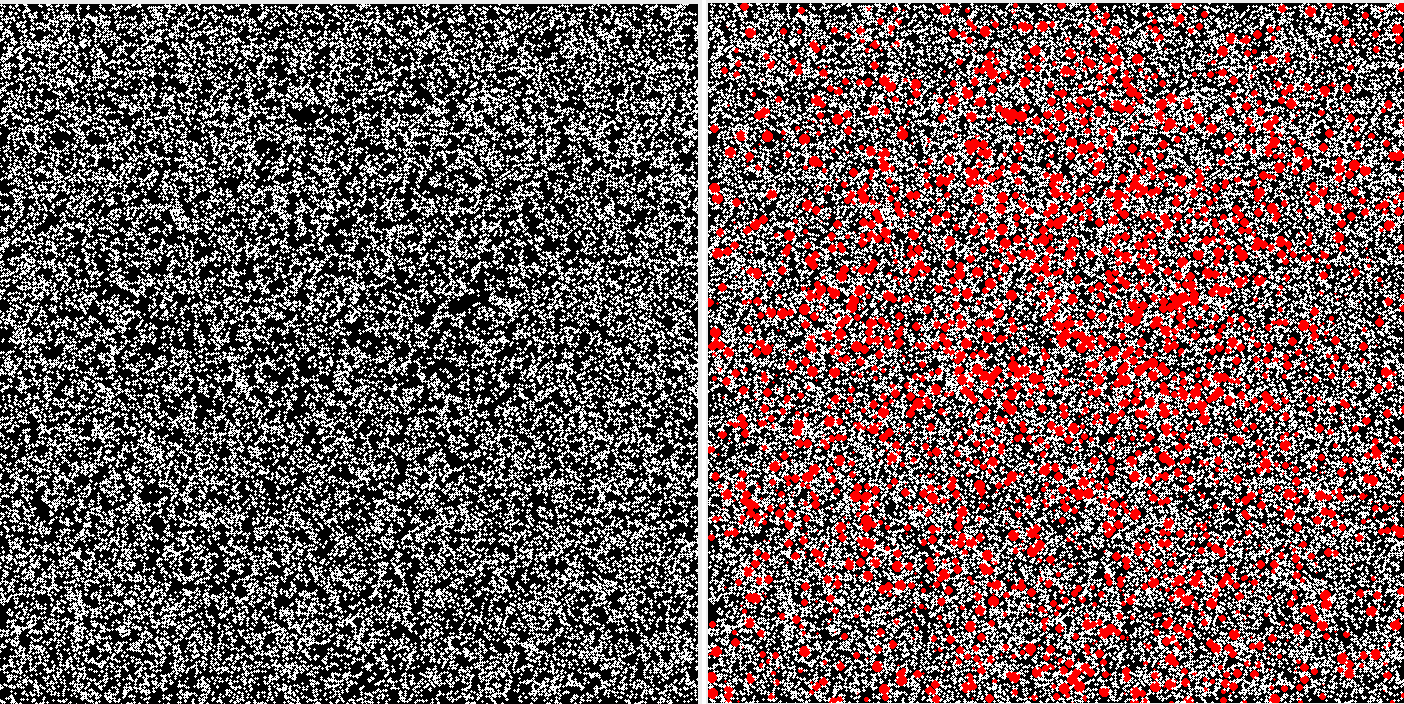
\includegraphics[width=\textwidth]{shade_propagation_test.png}
	\caption{ \textit{Shade Test: Results of a simulation run with \textit{S$_{smallroots}$} (red), grass (white) after 10 years. Top-left: Rendered with both species. Top-right: Only grass rendered in order to clearly visualise the empty areas at the exact locations the canopies of \textit{S$_{smallroots}$} appear. Bottom: The same simulation run with only grass, clearly showing the empty areas disappear.}} 
	\label{fig:shade_test}
\end{figure}

\textbf{SHADE-LOVING TEST}\\

As discussed in \ref{subsec:spawning_plants}, species which strive in shaded areas are deemed shade-loving. The shade can be caused by the terrain relief or by the shadow cast by the canopy of taller plants. To test whether the ecosystem simulator successfully caters for such plant species, a simulation identical to the shade test is run but with shade-loving species \textit{S$_{shadeloving}$} added (see appendix \ref{AppendixB} for species details). As seen by the snapshot of the simulation after fifteen years illustrated in figure \ref{fig:shade_loving_test}, instances of \textit{S$_{shadeloving}$} only appear in areas covered by the canopies of \textit{S$_{smallroots}$}.

\begin{figure}
\center
	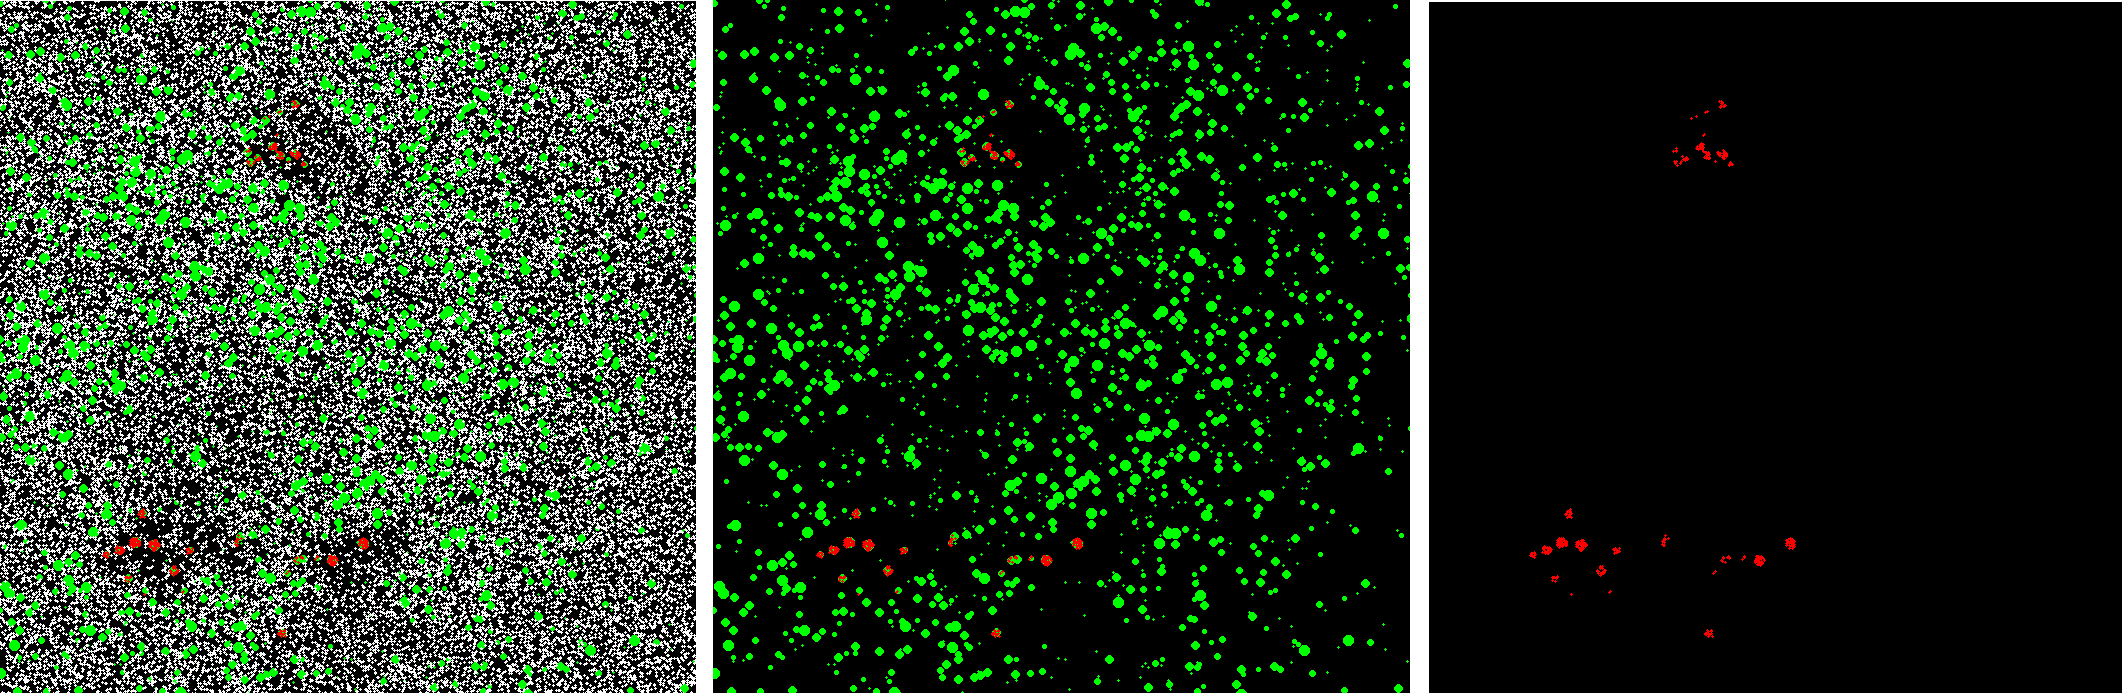
\includegraphics[width=\textwidth]{shade_loving_test.png}
	\caption{ \textit{Shade Loving Test: Simulation with \textit{S$_{smallroots}$} (red), grass (white) and \textit{S$_{shadeloving}$} (green) after 15 years. Left: All species rendered. Right: All except \textit{S$_{smallroots}$} rendered. It shows clearly that the only instances of \textit{S$_{shadeloving}$} which survive are those under the canopies of \textit{S$_{smallroots}$} (red).}}
	\label{fig:shade_loving_test}
\end{figure}

\section{Plant Distribution Analysis and Reproduction}

As mentioned previously, running a simulation using the ecosystem simulator to generate valid plant distributions can be a lengthy process (see section \ref{subsec:ecosytem_performance}). This processing time depends on the plant count and the resolution of the simulation window. The simulation illustrated in figure \ref{fig:ecosimulator_test_plant_count}, for example, took four and a half minutes to run.\\

The area to be covered by vegetation on the terrain, and therefore for which valid plant distributions created, is much larger than the hundred by hundred metre simulation window used in the ecosystem simulator. There are three obvious ways the ecosystem simulator could be used to generate vegetation for larger areas: \textit{Setting the simulation window to the area which must be covered}, \textit{decreasing the resolution of the simulation window} and by \textit{repeating the output of the hundred by hundred metre distribution (tiling)}. Each come with major setbacks, however, as \textit{increasing the simulation} window will further increase the processing time, \textit{decreasing the resolution} would impact the resulting realism and \textit{tiling} would create repetitive vegetation.\\

To attempt to generate vegetation which is coherent with that produced with the ecosystem but on a larger scale whilst minimizing impacts on performance and realism, the plant distribution output by the ecosystem simulator is analysed for later reproduction. The analysis and reproduction process are discussed in \textit{Analysis} and \textit{Reproduction} respectively.\\

The analysed distribution data, as well as permitting larger scale reproduction, can also be used as a cache mechanism to bypass future runs of the same ecosystem simulator run. Details on how this is implemented are discussed in \textit{Caching Distribution Data}.

To conclude this section, input exemplars will be analysed and the resulting reproduction(s) evaluated.

\subsection{Distribution Analysis}

\textit{Radial distribution analysis}, as described in section \ref{subsubsec:radial_distribution_analysis}, is performed on the output of the ecosystem simulator to grasp its core characteristics. Each plant instance acts as a single point and the different species represent the individual categories when performing the analysis. Customizations to the generic analysis algorithm are performed, however, to better suit the purpose of analysing plant distributions. Each are discussed separately below in: \textit{Generating the category hierarchy}, \textit{Category Dependency Analysis} and \textit{Point-size Analysis}. In \textit{Configuration Parameters} are discussed the parameters used. To conclude, the performance of the distribution will be discussed in \textit{Performance}.

\subsubsection{Generating the category hierarchy} \label{subsubsec:generating_cat_hierarchy}

During the reproduction phase, distributions for each category are created sequentially. One a valid distribution is created for a given category, it is static and \textbf{does not} change whilst points of other categories are being plotted. For this reason, the category hierarchy plays a vital role and has a big impact on the final distribution. A side effect of this hierarchical approach is that pair-correlation histograms do not need to be generated for each category pair combinations but only for combinations for which the target category is under or equal to the source category in the hierarchy.\\

Because taller plants will potentially have a canopy which shades and influences the position of smaller plants, it is important these be generated first during reproduction. For this reason, the hierarchy is generated according to the average height of the represented plant specie in descending order.

\subsubsection{Category Dependency Analysis} \label{subsubsec:category_dependency_analysis}

Shade-loving plants will appear under the the shaded canopies of taller plants (see section \ref{subsubsec:shade_loving_test}). When analysing the distance of these shade-loving plants to the plant's which shade them during the analysis phase, a new \textit{negative-bin} is created.\\

During reproduction, the taller plants will be generated first because they are classed higher in the hierarchy (see section \ref{subsubsec:generating_cat_hierarchy}). However, this does not guarantee all shade-loving plants will be placed in the shaded canopy of other plants as if a shade-loving plant is placed at a distance larger than \textit{R$_{max}$} to any other plant instance, it is attributed a strength of one and is therefore deemed valid. It is essential to attribute a strength of one in such condition to permit plant propagation. A solution to this problem would be to make \textit{R$_{max}$} large enough to cover the entire simulation window. This is extremely wasteful in terms of computational resources however and, as such, another solution is used here; When the pairwise histograms have been generated for a given category \textit{A}, they are analysed sequentially to check whether or not all instances appear within the \textit{negative-bin} of the other category (specie). The specie \textit{A} is deemed \textbf{dependent} on all categories for which this is true and, during reproduction, will have to be placed within the radius of one of them to be deemed valid.

\subsubsection{Point-size Analysis}

As well as the position of individual plants, an important property of the ecosystem simulator output is plant size. In order to reproduce appropriately sized plants, this must also be analysed. To do so, the \textit{minimum} and \textit{maximum} canopy radius and height for each category are also analysed.

\subsubsection{Configuration Parameters}

The \textit{radial distribution analysis} requires the following configuration parameters: \textit{R$_{min}$}, \textit{R$_{min}$} and \textit{bin-size}. Details on each parameter can be found in section \ref{subsubsec:radial_distribution_analysis}.\\

Increasing the analysis range [\textit{R$_{min}$}, \textit{R$_{max}$}] and decreasing the \textit{bin-size} will impact performance but potentially increase the accuracy of the analysis and finding optimal values for these parameters depends on the properties of the points being analysed.\\
It is unnecessary to have too large of an analysis range as the impact a plant has on it's surrounding is finite. This impact radius varies however and is dependent on specie size. In order to cater for different species of different sizes and therefore with different impact radii, R$_{max}$ is dynamic and limited to \textbf{two metres} passed the extremity of the plant's canopy.\\
The bin-size doesn't influence performance as severely as the analysis range, however, as it has no impact on the number of points that need to be processed. Smaller bin sizes will result in less points being processed per bin and, therefore, a less accurate representation of the distribution variation with distance. Because smaller bins will result in a smaller number of points, also, the analysis will be more sensitive to noise. A bin size of \textbf{twenty centimetres} is used as it strikes a good balance between accuracy and point count per bin. \\

\subsubsection{Performance} \label{subsubsec:analysis_performance}

In order to generate the necessary analysis data, each point (plant) must be iterated over and the distance measured from it to all other points within a radius of \textit{R$_{max}$}. As a consequence, the analysis time is directly correlated to plant density and, therefore, plant count within the hundred metre analysis window. To determine the correlation between plant density and analysis time, test distributions are generated of various densities using the ecosystem simulator which are subsequently analysed and the time to do so, measured. Because the number of histograms that need to be generated depends on the number of categories to be analysed, one would easily assume that the processing time is also correlated to the category count. This is \textbf{not} the case however and only point density influences analysis performance. To demonstrate this, the various plant densities are generated containing one, two and three distinct categories.The results plotted in figure \ref{fig:analysis_perf} indicate an exponential correlation between plant count and processing time and a quicker analysis time when points are split into multiple categories. Although the correlation is exponential, the most extreme scenario (over ninety thousand points of a single category) is processed in a manageable time of just under two seconds. 

\begin{figure}
\center
	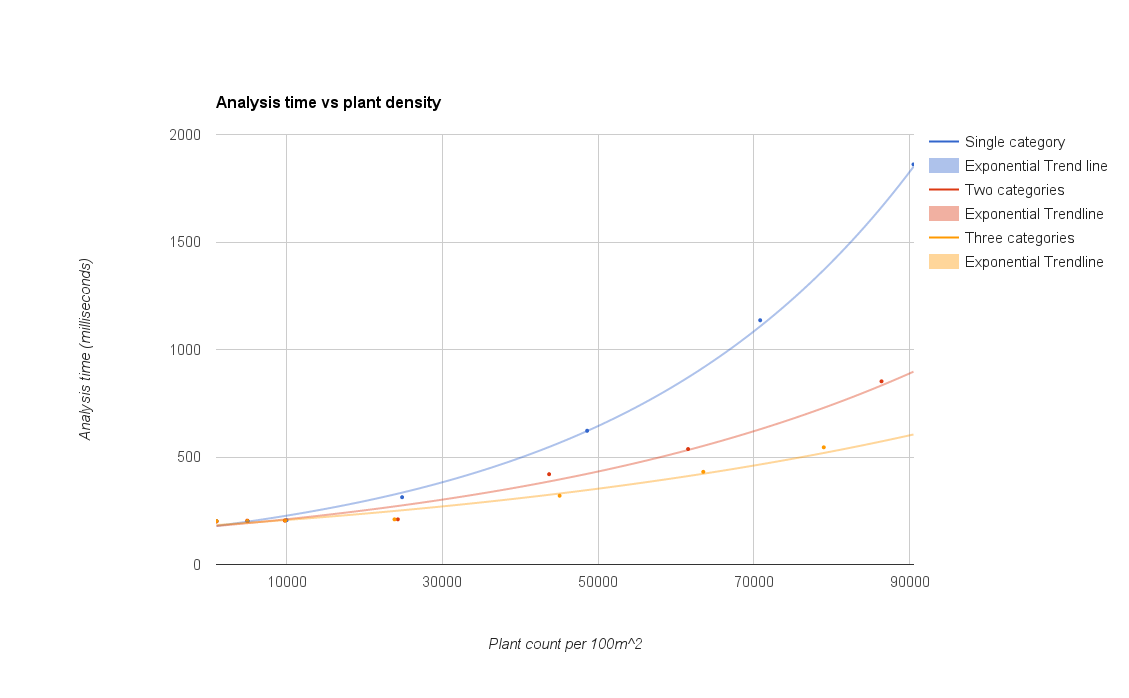
\includegraphics[width=\textwidth]{radial_distribution_analysis_performance.png}
	\caption{ Distribution analysis time based on aggregate plant density for single category (blue), two categories (red) and three categories (yellow).}	
	\label{fig:analysis_perf}
\end{figure}

\subsection{Reproduction}

The purpose of the analysed radial distribution data is to later use it to reproduce similar distributions on larger scales. To do so, the same reproduction technique described in section \ref{subsubsec:radial_distribution_analysis} is employed with slight nuances described below, namely: \textit{Matched-density initialization} and \textit{Iterative point moving}.\\

The radial distribution data generated to test the analysis performance above (section \ref{subsubsec:analysis_performance}) is used to test the reproduction performance.

\subsubsection{Matched Density Initialization}

Rather than employ a birth-and-death technique like that described in section \ref{subsubsec:radial_distribution_analysis}, where a point is added, the aggregate strength of the distribution calculated and the new point accepted with a calculated probability, matched-density initialization is employed. This involved generating a fixed number of points for each category so that their density matches that of the analysed density. The only requirement is for the aggregate strength of the distribution to be non-zero. In other words, the distribution does not need to be strongly matched, but valid.

\subsubsection{Iterative Point Moving} \label{subsubsec:iterative_point_moving}

When points of a given category have been initialized and the required density reached, iterative point-moving is performed where each added point is iterated over and moved to two random locations. The new distribution strength is calculated after each move and the best scoring move is accepted with probability \textit{P$_{acceptance}$}, calculated using equation \ref{eq:reproduction_probability_acceptance}. 

\begin{equation}
\centering
P_{acceptance} = \frac{Strength_{n+1}}{Strength_{n}}
\label{eq:reproduction_probability_acceptance}
\end{equation}
Where:
\begin{itemize}
\item \textit{Strength$_{n+1}$} is the aggregated distribution strength after the move.
\item \textit{Strength$_{n}$} is the aggregated distribution strength before the move.
\end{itemize}

\subsubsection{Performance}

The reproduction area and point density are two properties which greatly affect performance. Although both effect the number of points to reproduce and, therefore, the reproduction time, because an increase in density will lead to more points within R$_{max}$ of any given source point, given a fixed plant count, performance should increase with area. To determine to what extent and the correlation between plant density, reproduction area and performance, test reproductions are performed using the analysis data generated when performance testing the analysis stage (section \label{subsubsec:analysis_performance}).

As seen in figure \ref{fig:reproduction_density_area_perf} which plots the reproduction performance based on point density for various reproduction areas, the correlation between plant density and reproduction time is exponential. It also shows the increase to be more accentuated when reproducing larger areas. This is expected, however, as larger areas will require more points to be added in order to meet the required density.\\

\begin{figure}
\center
	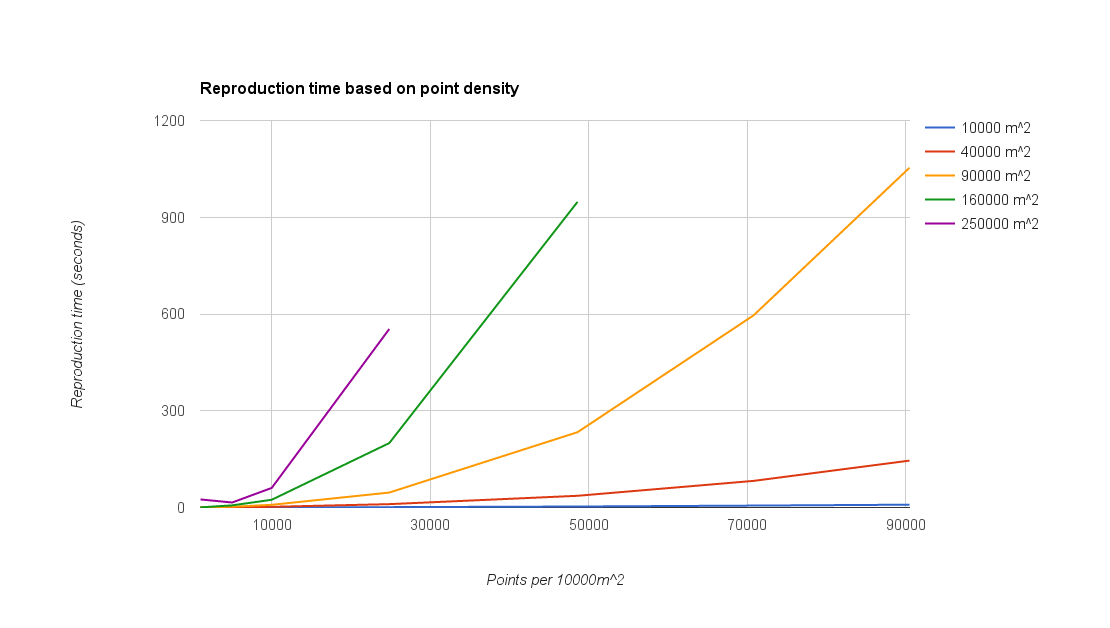
\includegraphics[width=\textwidth]{radial_distribution_reproduction_area_and_density_perf.png}
	\caption{ Reproduction time based on point density for different reproduction areas.}	
	\label{fig:reproduction_density_area_perf}
\end{figure}

Using the test data generated for figure \ref{fig:reproduction_density_area_perf}, it is possible to plot the reproduction time based solely on plant count for various densities (see figure \ref{fig:reproduction_plant_count_perf}). It shows the correlation between plant count and reproduction time to be linear and dependent on point density. The reason it is sensitive to plant density is because the denser the points are the the more of them will be within a distance of R$_{max}$ and therefore need ot be taken into consideration when calculating the strength of the distribution. In order to keep reproduction times manageable, the reproduced plant count is limited to half a million. If large areas need to be reproduced with a plant count higher than this limit, repeating/tiling is performed. Appendix \ref{AppendixC} outlines the maximum reproduction areas that can be achieved for different plant densities. Although the repetition (tiling) performed will increase for denser distributions, it will not necessarily be more noticeable as denser distributions will tend to have less distinct patterns and be more closely correlated to random.\\

\begin{figure}
\center
	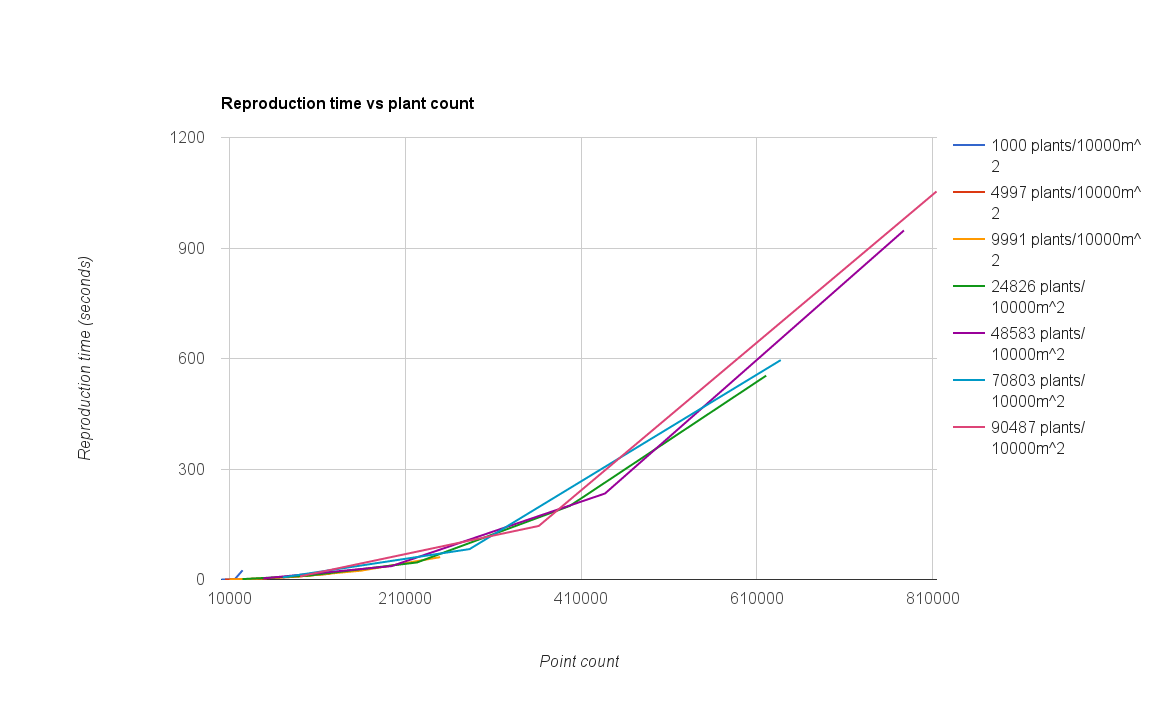
\includegraphics[width=\textwidth]{radial_distribution_reproduction_plant_count_perf.png}
	\caption{ Reproduction time based on point count for different densities.}	
	\label{fig:reproduction_plant_count_perf}
\end{figure}

\subsection{Caching Distribution Data}

In order to prevent repeated costly runs of the ecosystem simulator for identical resource parameters, the analysed distribution data is stored and tracked in a database. This way, if a plant distribution is requested for a simulation which has already been run, the ecosystem simulator is bypassed entirely and the stored distribution data used. A custom binary file format is used in order to save space when storing the necessary analysed distribution data.

\subsection{Results}

The important properties of the input exemplars which must be reproduced are: \textit{inter and intra specie separation}, \textit{plant size} and \textit{specie densities}. To ensure these are accurately reproduced, an ecosystem simulator run is performed containing \textit{shade-loving}, \textit{shade intolerant} and \textit{canopy plants}. The resulting plant distribution is subsequently used as input exemplar to stress test the distribution analyser and reproducer. Figure \ref{fig:radial_dist_test} shows an overview and zoomed subsection of the input exemplar along with it's associated reproduction. From this, along with the point count of individual species, it is possible to conclude that point density and point size is accurately replicated. To determine whether intra and inter-specie spacing is accurately reproduced, the reproduction distribution is re-analysed in order to produce the pair correlation histograms of the reproduced distribution. The original and reproduced histograms are then compared to ensure they follow similar trends (see figure \ref{fig:hisogram_comp}). Important properties to note which are accurately reproduced are:
\begin{itemize}
\item No plants appear within the radius of the shade-loving (category 6) and shade-intolerant plants (category 5)
\item The density of shade-intolerant plants (category 5) drastically decreases within the radius of canopy plants (category 9).
\item The density of shade-loving plants (category 6) drastically decreases within the radius of canopy plants (category 9). Note that in both the original and reproduction, all shade-loving plants appear within the radius of a canopy plants as the categories are dependent (see section \ref{subsubsec:category_dependency_analysis}). The variation in histogram values between the two is caused by the positioning of other nearby canopy plants.
\item The density decreases drastically for canopy plants within the canopy of other canopy plants (category 9) as it blocks access to available illumination.
\end{itemize}

Note that the pair correlation histogram of the shade-loving specie with itself (category 6 and 6) is substantially different between original and reproduction. The reason for this is because during the ecosystem simulator, seeding is performed from existing plant instances which will lead to the clustering of plants under the same canopy. During iterative point-moving (see section \ref{subsubsec:iterative_point_moving}, the probability of shade-loving plants to cluster under neighbouring canopy plants is very slim, however, and dispersion under all present canopy plants is much more likely.

\begin{figure}
\center
	\includegraphics[width=\textwidth]{radial_distribution_test_general_comp.png}
	\caption{ Distribution analysis and reproduction test: Input exemplar overview (top-left), reproduction overview (top right), zoomed input exemplar (x 10), zoomed reproduction (x 10). }	
	\label{fig:radial_dist_test}
\end{figure}

\begin{figure}
\center
	\includegraphics[width=\textwidth]{radial_dis_reprod_test_hist_aggregated.png}
	\caption{ Original (blue) and reproduced (red) pair correlation histograms for different bins where category 6 is a shade-loving, category 5 is shade intolerant and category 9 is a canopy specie. Bin sizes of -1 signify the target category is within the radius of the source.}	
	\label{fig:hisogram_comp}
\end{figure}


\begin{appendices}
\chapter{Cluster Summary} \label{AppendixA}

\definecolor{cluster_1}{rgb}{0.8,0.4,0.0}
\definecolor{cluster_2}{rgb}{0.6,0.4,0.4}
\definecolor{cluster_3}{rgb}{0.0,0.2,0.4}
\definecolor{cluster_4}{rgb}{1.0,1.0,0.4}
\definecolor{cluster_5}{rgb}{0.0,0.6,1.0}
\begin{table}[]
  \centering
	    \begin{tabular}{|p{5cm}|p{2cm}|p{2cm}|p{2cm}|p{2cm}|p{2cm}|}
		\hline	
  	     & \textbf{1} &  \textbf{2} & \textbf{3} & \textbf{4} & \textbf{5} \\
		\hline
  	    Color & \cellcolor{cluster_1} & \cellcolor{cluster_2} & \cellcolor{cluster_3} & \cellcolor{cluster_4} & \cellcolor{cluster_5} \\
		\hline
  	    Member count & 7233 (0.7\%)  & 203043 (19\%) & 119853 (11\%)  & 271116 (26\%) & 447331 (43\%) \\
		\hline
  	    Slope & 18.5967 & 36.6987 & 56.9893 & 18.7228 & 5.9857 \\
		\hline
  	    Temperature (Jan) & 0 & -1 & -1 & 25 & 23 \\
		\hline
  	    Temperature (Feb) & 3 & 1 & 1 & 23 & 21 \\
		\hline
  	    Temperature (Mar) & 5 & 3 & 3 & 2 & 0 \\
		\hline
  	    Temperature (Apr) & 8 & 6 & 6 & 5 & 3 \\
		\hline
  	    Temperature (May) & 10 & 8 & 8 & 7 & 5 \\
		\hline
		Temperature (Jun) & 13 & 11 & 11 & 10 & 8 \\
		\hline
		Temperature (Jul) & 10 & 8 & 8 & 7 & 5 \\
		\hline
		Temperature (Aug) & 8 & 6 & 6 & 5 & 3 \\
		\hline
		Temperature (Sep) & 5 & 3 & 3 & 2 & 0 \\
		\hline
		Temperature (Oct) & 3 & 1 & 1 & 0 & -2 \\
		\hline
		Temperature (Nov) & 0 & -1 & -2 & -2 & -4 \\
		\hline
		Temperature (Dec) & -2 & -4 & -4 & -5 & -7 \\
		\hline
  	    Illumination (Jan) & 7 & 8 & 6 & 9 & 10 \\
		\hline
  	    Illumination (Feb) & 7 & 8 & 6 & 9 & 10 \\
		\hline
  	    Illumination (Mar) & 7 & 8 & 7 & 9 & 10 \\
		\hline
  	    Illumination (Apr) & 7 & 8 & 6 & 9 & 10 \\
		\hline
  	    Illumination (May) & 7 & 7 & 6 & 9 & 10 \\
		\hline
		Illumination (Jun) & 6 & 7 & 5 & 8 & 10 \\
		\hline
		Illumination (Jul) & 7 & 7 & 6 & 9 & 10 \\
		\hline
		Illumination (Aug) & 7 & 8 & 6 & 9 & 10 \\
		\hline
		Illumination (Sep) & 7 & 8 & 7 & 9 & 10 \\
		\hline
		Illumination (Oct) & 7 & 8 & 6 & 9 & 10 \\
		\hline
		Illumination (Nov) & 7 & 8 & 6 & 9 & 10 \\
		\hline
		Illumination (Dec) & 6 & 7 & 5 & 8 & 10 \\
		\hline
  	    Soil Humidity (Jan) & 674.9 & 3.9 & 1.8 & 14.3 & 13.6 \\
		\hline
  	    Soil Humidity (Feb) & 693.0 & 4.2 & 1.9 & 15.5 & 14.8 \\
		\hline
  	    Soil Humidity (Mar) & 691.8 & 4.1 & 1.9 & 15.1 & 14.4 \\
		\hline
  	    Soil Humidity (Apr) & 647.6 & 3.5 & 1.6 & 12.6 & 11.9 \\
		\hline
  	    Soil Humidity (May) & 572.3 & 2.6 & 1.3 & 9.1 & 8.5 \\
		\hline
  	    Soil Humidity (Jun) & 625.4 & 3.7 & 1.8 & 13.5 & 12.8 \\
		\hline
  	    Soil Humidity (Jul) & 675.8 & 4.6 & 2.1 & 17.2 & 16.4 \\
		\hline
  	    Soil Humidity (Aug) & 713.1 & 5.8 & 2.6 & 21.6 & 20.6 \\
		\hline
  	    Soil Humidity (Sep) & 705.0 & 5.1 & 2.3 & 19.2 & 18.3 \\
		\hline
  	    Soil Humidity (Oct) & 672.8 & 4.2 & 2.0 & 15.2 & 14.5 \\
		\hline
  	    Soil Humidity (Nov) & 630.9 & 3.2 & 1.6 & 11.5 & 10.9 \\
		\hline
  	    Soil Humidity (Dec) & 659.2 & 3.8 & 1.8 & 13.8 & 13.1\\
		\hline
		\end{tabular}
		\caption{Clustering test: Cluster summary.}
	  \label{tab:clustering_test_resulting_clusters}
\end{table}
\chapter{Species Properties} \label{AppendixB}

\begin{longtable}{|p{3cm}|p{1cm}|p{1cm}|p{1cm}|p{1cm}|p{1cm}|p{1cm}|p{2cm}|p{2cm}|}
		\hline		
		\textbf{Name} & \textbf{Grass} & \textbf{S$_{base}$} & \textbf{S$_{X2}$} & \textbf{S$_{X3}$} & \textbf{S$_{slow}$} & \textbf{S$_{fast}$} & \textbf{S$_{smallroots}$} & \textbf{S$_{shadeloving}$}\\
		\hline
		\textbf{Max Height (cm)} & 60 & 1500 & 1500 & 1500 & 1500 & 1500 & 1500 & 50 \\
		\hline
		\textbf{Max canopy width (cm)} & 0 & 1000 & 2000 & 3000 & 2000 & 2000 & 3000 & 0 \\
		\hline
		\textbf{Max root size (cm)} & 20 & 1000 & 2000 & 2000 & 2000 & 2000 & 50 & 30 \\
		\hline
		\textbf{Age of start of decline (months)} & 8000 & 1000 & 1000 & 1000 & 500 & 300 & 1000 & 1000 \\
		\hline
		\textbf{Maximum age (months)} & 9000 & 2000 & 2000 & 2000 & 600 & 350 & 2000 & 2000 \\
		\hline
		\textbf{Start of prime illumination (h)} & 8 & 8 & 8 & 8 & 8 & 8 & 8 & 0 \\
		\hline
		\textbf{End of prime illumination (h)} & 12 & 12 & 12 & 12 & 12 & 12 & 12 & 4 \\
		\hline
		\textbf{Minimum illumination (h)} & 5 & 6 & 6 & 6 & 3 & 6 & 6 & 0 \\
		\hline
		\textbf{Maximum illumination (h)} & 15 & 12 & 12 & 12 & 12 & 12 & 12 & 6 \\ 
		\hline
		\textbf{Start of prime humidity (mm)} & 25 & 25 & 25 & 25 & 25 & 25 & 25 & 10 \\
		\hline
		\textbf{End of prime humidity (mm)} & 45 & 35 & 35 & 35 & 35 & 35 & 35 & 25 \\
		\hline
		\textbf{Minimum humidity (mm)} & 10 & 15 & 15 & 15 & 15 & 15 & 15 & 5 \\
		\hline
		\textbf{Maximum humidity (mm)} & 60 & 45 & 45 & 45 & 45 & 45 & 45 & 40 \\
		\hline
		\textbf{Start of prime temperature (degrees)} & 15 & 10 & 10 & 10 & 10 & 10 & 10 & 10 \\
		\hline
		\textbf{End of prime temperature (degrees)} & 25 & 20 & 20 & 20 & 20 & 20 & 20 & 20 \\
		\hline
		\textbf{Minimum temperature (degrees)} & 0 & -5 & -5 & -5 & -5 & -5 & -5 & -10 \\
		\hline
		\textbf{Maximum temperature (degrees)} & 40 & 30 & 30 & 30 & 30 & 30 & 30 & 30 \\
		\hline
		\textbf{Maximum seeding distance (m)} & 3 & 50 & 50 & 50 & 50 & 50 & 50 & 3 \\
		\hline
		\textbf{Annual seed count} & 1000 & 100 & 100 & 100 & 100 & 100 & 100 & 1000 \\
		\hline                                                                           
\end{longtable}
\chapter{Maximum Distribution Reproduction Areas} \label{AppendixC}

\begin{longtable}{|p{7cm}|p{8cm}|}
		\hline
		\textbf{Points per 10000m$^{2}$} & \textbf{Maximum reproduction area (m$^{2}$)}\\
		\hline
		5000	  &  1000000\\
		\hline
		10000	  &  500000\\
		\hline
		15000 &	333333\\
		\hline
		20000 &	250000\\
		\hline
		25000 &	200000\\
		\hline
		30000 &	166666\\
		\hline
		35000 &	142857\\
		\hline
		40000 &	125000\\
		\hline
		45000 &	111111\\
		\hline
		50000 &	100000\\
		\hline
		55000 &	90909\\
		\hline
		60000 &	83333\\
		\hline
		65000 &	76923\\
		\hline
		70000 &	71428\\
		\hline
		75000 &	66666\\
		\hline
		80000 &	62500\\
		\hline
		85000 &	58823\\
		\hline
		90000 &	55555\\
		\hline
		95000 &	52631\\
		\hline
		100000 & 50000\\
		\hline
		\caption{Maximum reproduction area for given plant densities}
	  \label{tab:maximum_reproduction_areas}
\end{longtable}
\chapter{Machine Specifications} \label{AppendixD}

\begin{table}[]
  \centering
	    \begin{tabular}{|p{8cm}|p{8cm}|}
	    \hline
	    \textbf{CPU} & Intel Core i7-4770 CPU @ 3.40GHz\\
	    \hline
	    \textbf{GPU} & Nvidia GeForce GTX 770\\
	    \hline
	    \textbf{RAM} & \\
	    \hline
	    \textbf{Storage} & 1TB HDD + 60GB SDD\\
		\end{tabular}
		\caption{Specifications of the machine used for all performance testing.}
	  \label{tab:maximum_reproduction_areas}
\end{table}
\end{appendices}

\bibliographystyle{alpha}
\bibliography{MyCollection}{}
\end{document}